%*******************************************************************************
%*********************************** Chapter DUNE ******************************
%*******************************************************************************
\chapter{The Deep Underground Neutrino Experiment}  ~\label{chap:DUNE} %Title of chapter

\graphicspath{{DUNE/Figs/PDF/}{DUNE/Figs/Raster/}{DUNE/Figs/Vector}}

%%% The main DUNE section
\nomenclature[z-FD]{FD}{Far Detector}
\nomenclature[z-ND]{ND}{Near Detector}
\nomenclature[z-FNAL]{FNAL}{Fermi National Lab}
\nomenclature[z-Fermilab]{Fermilab}{Fermi National Lab}
\nomenclature[z-DUNE]{DUNE}{Deep Underground Neutrino Experiment}
\nomenclature[z-LBNF]{LBNF}{Long Baseline Neutrino Facility}
\nomenclature[z-LBNF]{LBNE}{Long Baseline Neutrino Experiment}
\nomenclature[z-LBNF]{LBNO}{Long Baseline Neutrino Observatory}
\nomenclature[z-SURF]{SURF}{Sanford Underground Research Facility}
\nomenclature[z-PIP-II]{PIP-II}{Proton Improvement Plan II}
\nomenclature[z-CDR]{CDR}{Conceptual Design Review}

%% Single Phase detector
\nomenclature[z-APA]{APA}{Anode Plane Assembly}
\nomenclature[z-CPA]{CPA}{Cathode Plane Assembly}
\nomenclature[z-PD]{PD}{Photon Detector}
\nomenclature[z-PCB]{PCB}{Printed Circuit Board}
\nomenclature[z-SiPM]{SiPM}{Silicon Photo Multiplier}
\nomenclature[z-SSP]{SSP}{SiPM Signal Processor}

%% Dual Phase detector
\nomenclature[z-LEM]{LEM}{Large Electron Multipliers}
\nomenclature[z-CRP]{CRP}{Charge Readout Planes}
\nomenclature[z-LAS]{LAS}{LEM/Anode Sandwiches}
\nomenclature[z-PMT]{PMT}{Photo Multiplier Tubes}

%% The near detector
\nomenclature[z-FGT]{FGT}{Fine-Grained Tracker}
\nomenclature[z-ECal]{ECal}{Electromagnetic Calorimeter}
\nomenclature[z-RPC]{RPC}{Resistive Plate Chambers}

%% The 35 ton detector
\nomenclature[z-CRC]{CRC}{Cosmic Ray Counter}

%%% LArSoft section
\nomenclature[z-LArSoft]{LArSoft}{Liquid Argon Software}
\nomenclature[z-\emph{art}]{\emph{art}}{\emph{analysis reconstruction framework}}
\nomenclature[a-tick]{tick}{Unit of time equal to 500 ns}
\nomenclature[z-ADC]{ADC}{Analogue to Digital Converter}
%% My generators
\nomenclature[z-CRY]{CRY}{Cosmic-ray Shower Library}
\nomenclature[z-GENIE]{GENIE}{Generates Events for Neutrino Interaction Experiments}
\nomenclature[z-MUSUN]{MUSUN}{MUon Simulations UNderground}
\nomenclature[z-MUSIC]{MUSIC}{MUon Simulation Code}
%\nomenclature[z-CORSIKA]{CORSIKA}{COsmic Ray SImulations for KAscade}

The Deep Underground Neutrino Experiment (DUNE) is a next-generation neutrino experiment, which came about through the recommendations of the P5 report in 2014~\citep{P5Doc}. It was largely formed by the merger of two competing next-generation neutrino experiments, the Long Baseline Neutrino Experiment (LBNE)~\citep{LBNE_CDR1, LBNE_CDR2, LBNE_CDR3, LBNE_CDR4, LBNE_CDR5, LBNE_CDR6} a US-based experiment, and the Long Baseline Neutrino Observatory (LBNO)~\citep{LBNO_EOI} a European-based experiment. \\

The DUNE Far Detector (FD) will consist of four modules, each of which is a 10 kt Liquid Argon (LAr) Time Projection Chamber (TPC) (LArTPC). The four FD modules will be 4850 ft below ground, at the Sanford Underground Research Facility (SURF). This detector location is 1300 km away Fermi National Lab (FNAL, Fermilab), from which DUNE will receive a neutrino beam with a beam power of 1.2 MW, this will increase to 2.4 MW during the lifetime of the experiment. There will also be a high resolution, and high precision, Near Detector (ND) located at Fermilab. A schematic of the DUNE experimental setup is shown in Figure~\ref{fig:DUNESchematic}. Given this experimental setup, DUNE will have a wide range of physics opportunities, these are discussed in detail in Section~\ref{sec:DUNEPhys}. There is extensive documentation concerning all aspects of DUNE, this can be found in a suite of four Conceptual Design Review (CDR) documents~\citep{DUNECDR_V1, DUNECDR_V2, DUNECDR_V3, DUNECDR_V4}, and numerous annexes~\citep{DUNEAtWork}. What follows is a high level summary of the information contained in these CDR volumes, and annexes. \\ 

\begin{figure}
  \centering
  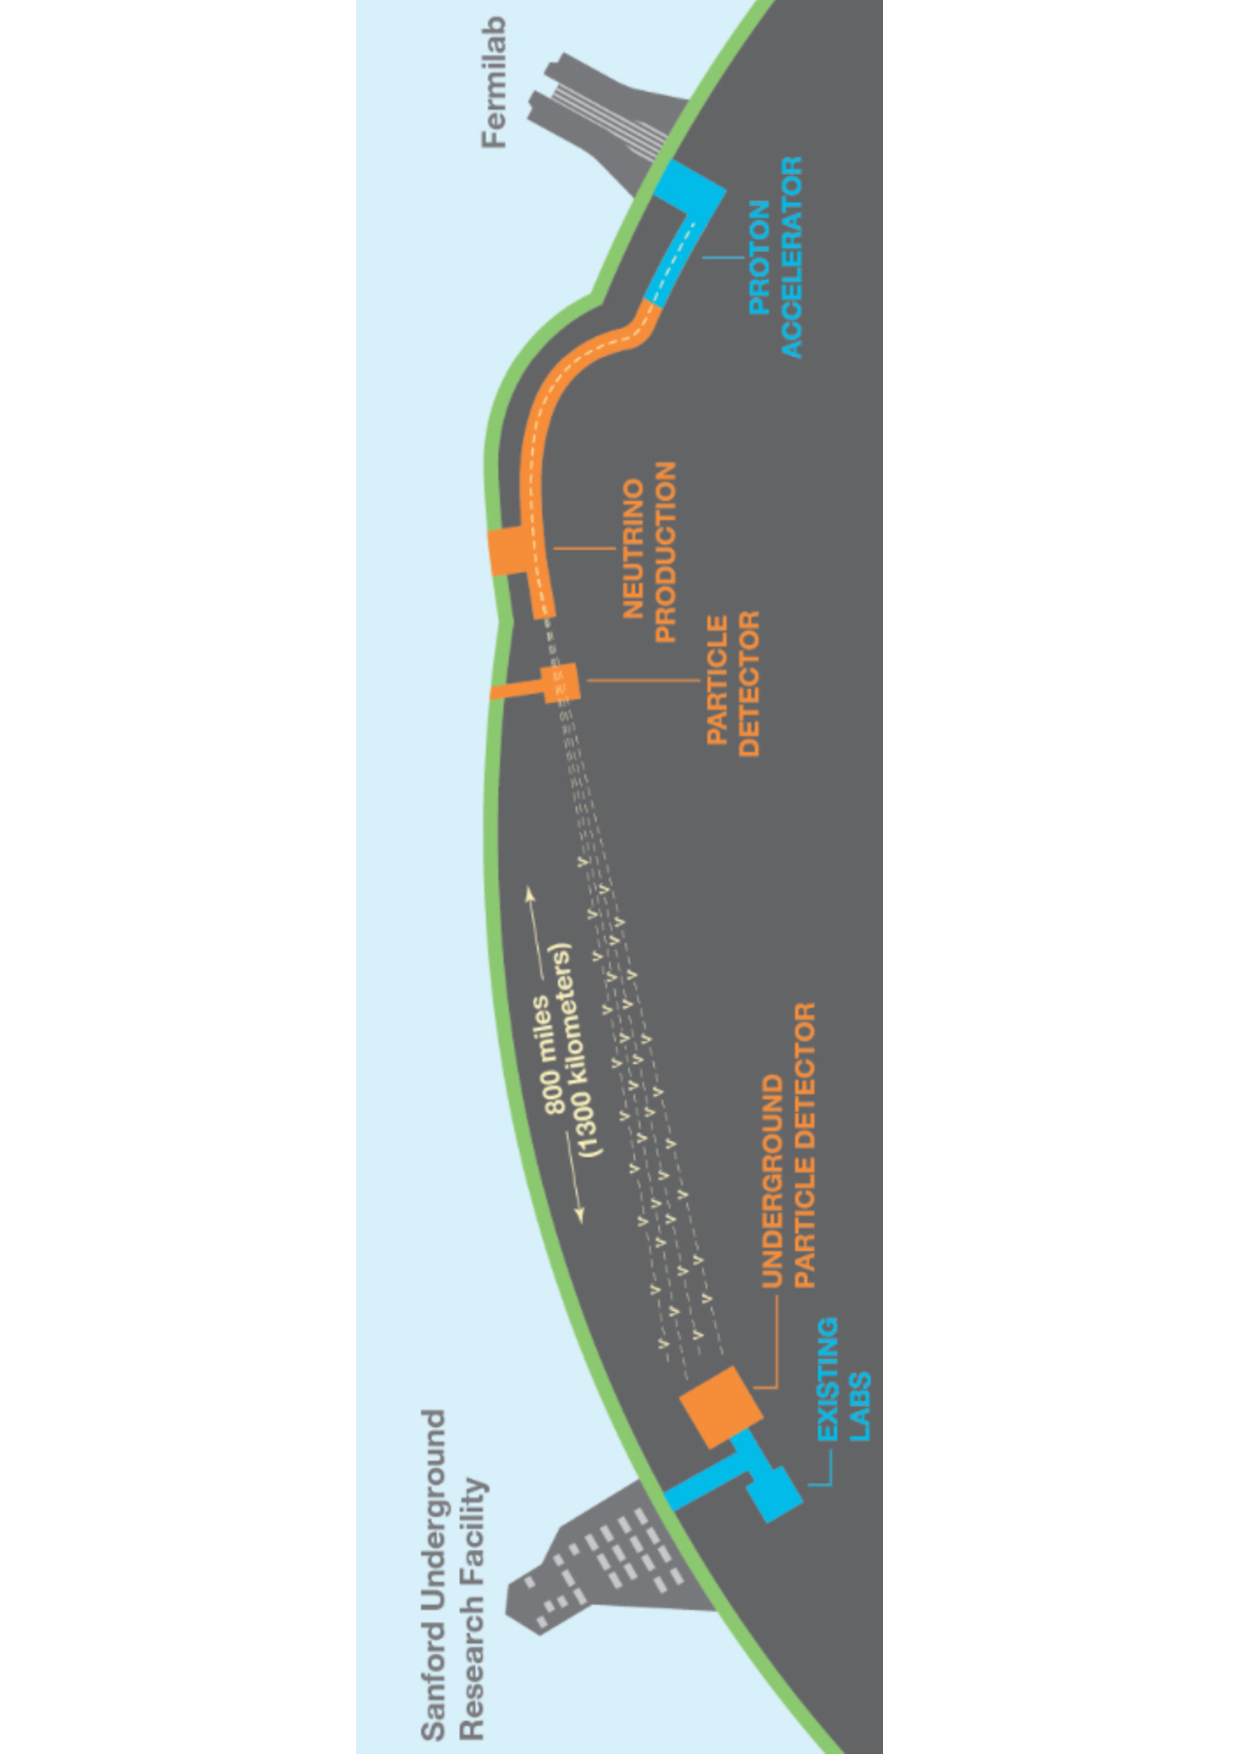
\includegraphics[width=0.9\textwidth]{DUNESchematic}
  \caption[A representation of the DUNE experimental setup]
          {A representation of the DUNE experimental setup. Fermilab, the host lab is shown right. The neutrino beam will be produced at Fermilab, and a high resolution near detector will also be located there. SURF is shown left, this is 1300 km away from Fermilab, and is where the far detector will be located. Objects in orange need to be built during the lifetime of the experiment, whilst objects in blue already exist. The figure is not to scale, and is taken from~\citep{DUNECDR_V1}.}
  \label{fig:DUNESchematic}
\end{figure}

%********************************** %Second Section  *************************************
\section{The DUNE schedule} \label{sec:DUNESched} %Section - X.3
As DUNE is a very large project it requires extensive planning, so that man-power can be used effectively. This planning has to outline the expected timescales of when the beamline, and the numerous detectors, will become operational. A high level summary of the DUNE schedule is shown in Figure~\ref{fig:DUNE_Sched}, the efforts at both SURF (top) and Fermilab (bottom) are shown, as well as the numerous reviews DUNE has to be complete. \\ 

\begin{figure}
  \centering
  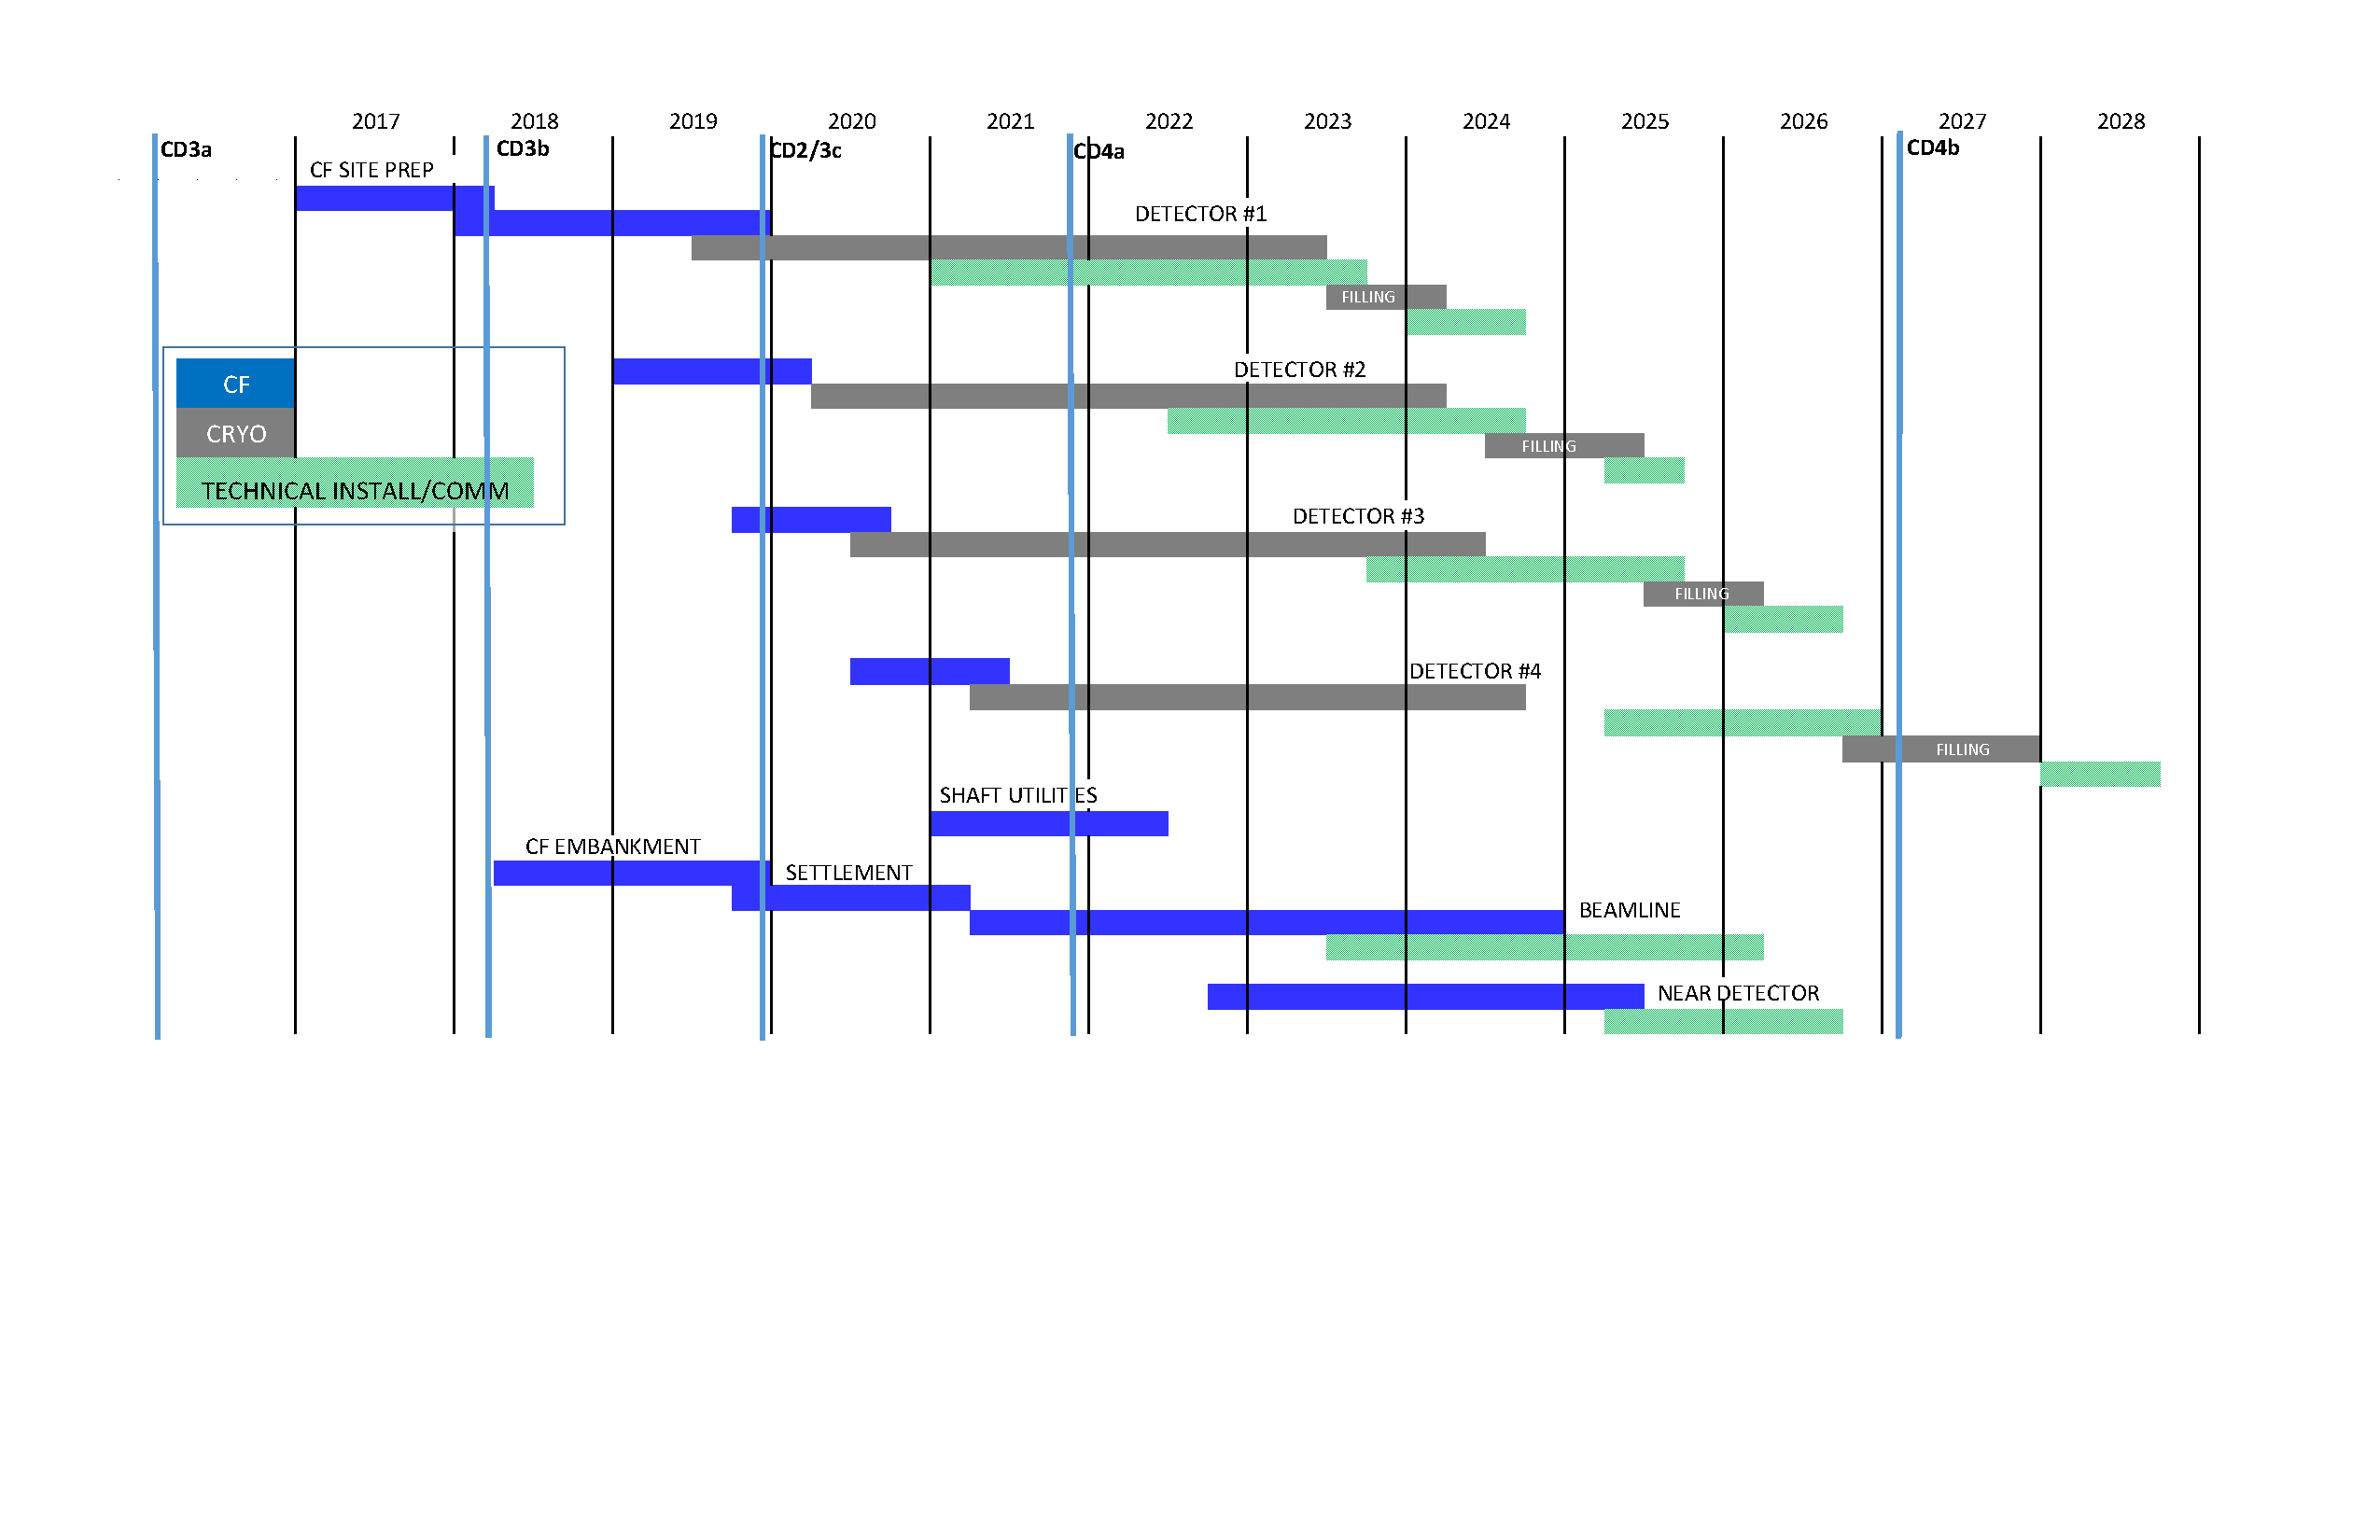
\includegraphics[width=\textwidth]{summary-schedule}
  \caption[A high level summary of the DUNE schedule]
          {A high level summary of the DUNE schedule. The phased construction of the four FD modules can be seen, with two of the four modules being commissioned before the beam becomes operational in 2026. The time required for construction of the facilities required for the detectors, and the beamline, are shown as blue boxes. The time required for the installation of cryogenic equipment, and filling, are shown as grey boxes. The time required for installation and commissioning, are shown as green boxes. The figure is taken from~\citep{DUNECDR_V1}.}
  \label{fig:DUNE_Sched}
\end{figure}

Figure~\ref{fig:DUNE_Sched} shows that when the beam becomes fully operational in 2026, two of the four 10 kt modules will have been fully commissioned, and will be ready to take beam data. Shortly after the beam becomes operational, the ND will also become operational, allowing the full physics scope of DUNE to begin to be realised. Following this, it is envisioned that the third and fourth detectors will become operational before the end of 2028. One thing which is not shown on the figure, is the planned upgrade of the beam to 2.14 MW, this is currently assumed to happen in 2032. This staged approach is necessary both from logistical, and physics positions, as it would be very difficult to build all four detectors simultaneously, and staging allows for improvements to be iteratively made in the construction of the TPCs in each of the four modules. A staged approach is also beneficial from a physics position, as it means that the first 10 kt module will begin taking physics data in 2024, two years before the beamline is completed. This physics data will be using atmospheric and solar neutrinos, as well as looking for signals from supernova and proton decays. \\

%********************************** %First Section  **************************************
\section{LBNF - the DUNE detector location and neutrino beam} \label{sec:DUNE_LBNF} %Section - X.1 
Formally the preparation of the far detector site of DUNE, and the construction of the beam line which DUNE will use, do not fall under the remit of DUNE. This is because what may be thought of as the DUNE 'project' is formally split into two separate projects. One of these projects, the experiment called DUNE, is responsible for~\citep{DUNECDR_V1}:
\begin{itemize}
\item The scientific research goals which the experiment aims to accomplish, as well as the program needed to achieve this.
\item Formulating the technical requirements needed from the beamline in order to satisfy the physics goals outlined above.
\item The design, building, and maintenance, of the far and near detector systems, in order to achieve the physics program outlined above.  
\end{itemize}
The other project, the Long Baseline Neutrino Facility (LBNF), is responsible for~\citep{DUNECDR_V1}:
\begin{itemize}
\item The design, and construction of a 1.2 MW neutrino beam, utilising the Proton Improvement Plan II (PIP-II) upgrade at Fermilab~\citep{PIP-II}.
\item The civil construction for the near detector site.
\item The excavation of the far detector site, and the preparation of the caverns for the detector modules, including the cryostats and cryogenic systems, needed by the DUNE FDs.
\end{itemize}
As such, the design and construction of the neutrino beam, as well as the preparation of both the near and far detector sites, is not within the remit of responsibility for DUNE, but is instead under the remit of LBNF. This model, whereby there are two separate projects, one responsible for the facilities used in the experiment, and another, responsible for the design, construction, and maintenance of the experiments, is the model used at CERN, for the LHC and its associated experiments. Fermilab, as the host lab for LBNF, is thus intimately involved in LBNF, as CERN was in the completion of the LHC. \\

A discussion of the wider DUNE experiment is clearly not possible without first discussing the facilities which LBNF is responsible for building. What follows is thus a brief discussion of the LBNF project. \\

As will be discussed in Section~\ref{sec:DUNEPhys}, DUNE is first and foremost, a neutrino oscillation experiment, and so it is important to select a far detector location which allows for the largest possible physics opportunities. When a detailed study was performed by the LBNE collaboration to determine the location of the far detector for that experiment, it was determined that the Homestake Mine at SURF was the most optimal site~\citep{LBNEReconfig}. The reason for this was that this baseline allowed LBNE to deliver the full physics potential which it had hoped to be able to accomplish, see Section~\ref{sec:DUNEPhys}. It was further noted that this detector location could be the ``start of a long-term world-leading program...with subsequent phases.'' Following the formation of DUNE a similar review was performed, and the conclusion reached was that the FD site chosen by LBNE, was also the location at which DUNE could best achieve its physics goals. This determination was made under the remit that the subsequent phases outlined by the LBNE reconfiguration report were performed. These were that a highly capable near detector is built, that the FD consists of at least 35 kton at the 4850 ft level, and that a multi-MW beamline is used. \\

SURF is located in Lead, South Dakota, and is the refurbished Homestake gold mine. Upon mining operations finishing, the mine became briefly disused before being reopened as the Deep Underground Science and Engineering Laboratory (DUSEL). When funding for DUSEL ceased, the US Department of Energy (DOE), through Lawrence Berkeley National Lab agreed to support ongoing research efforts, thus SURF was created~\citep{SURFWebsite}. DUNE will be located near the Ross shaft, one of two shafts which go to the 4850 level. Near the other shaft, the Yates Shaft, is what is now called the Davis Campus, named after Ray Davis who performed the experiment bearing his name at the Homestake mine in the late 1960's~\citep{RayDavis1968, RayDavis1988}. \\

In order to prepare SURF for an experiment of the size of DUNE, a major renovation effort is required. This is because both shafts down to the 4850 level need to be reinforced to be able to cope with the amount of rock which has to be excavated, and the amount of building materials which need to brought down to the 4850 level to build the DUNE detectors, and cryogenic equipment~\citep{DUNECDR_V3}. Before excavation could occur extensive studies were required, this was to ensure that the rock around the proposed cavern system is of high enough quality to accommodate the cavern system required for DUNE. These studies confirmed that the chosen site was suitable~\citep{DUNECDR_V3}. \\

The dimensions of the cavern system which need to be excavated in order to accommodate the DUNE detectors is shown in Figure~\ref{fig:DUNECavernSystem}. From Figure~\ref{fig:DUNECavernSystem} it can be seen that the DUNE FDs will be located in two large caverns, either side of a central reservation, with each cavern housing two detector pits. Each detector will be contained within a self-standing, steel framed structure, within this structure will be a membrane cryostat which will house a total of 17.1 kt of LAr~\citep{DUNECDR_V3}. Further information regarding the DUNE FDs can be found in Section~\ref{sec:DUNEDetector}. \\

\begin{figure}
  \centering
  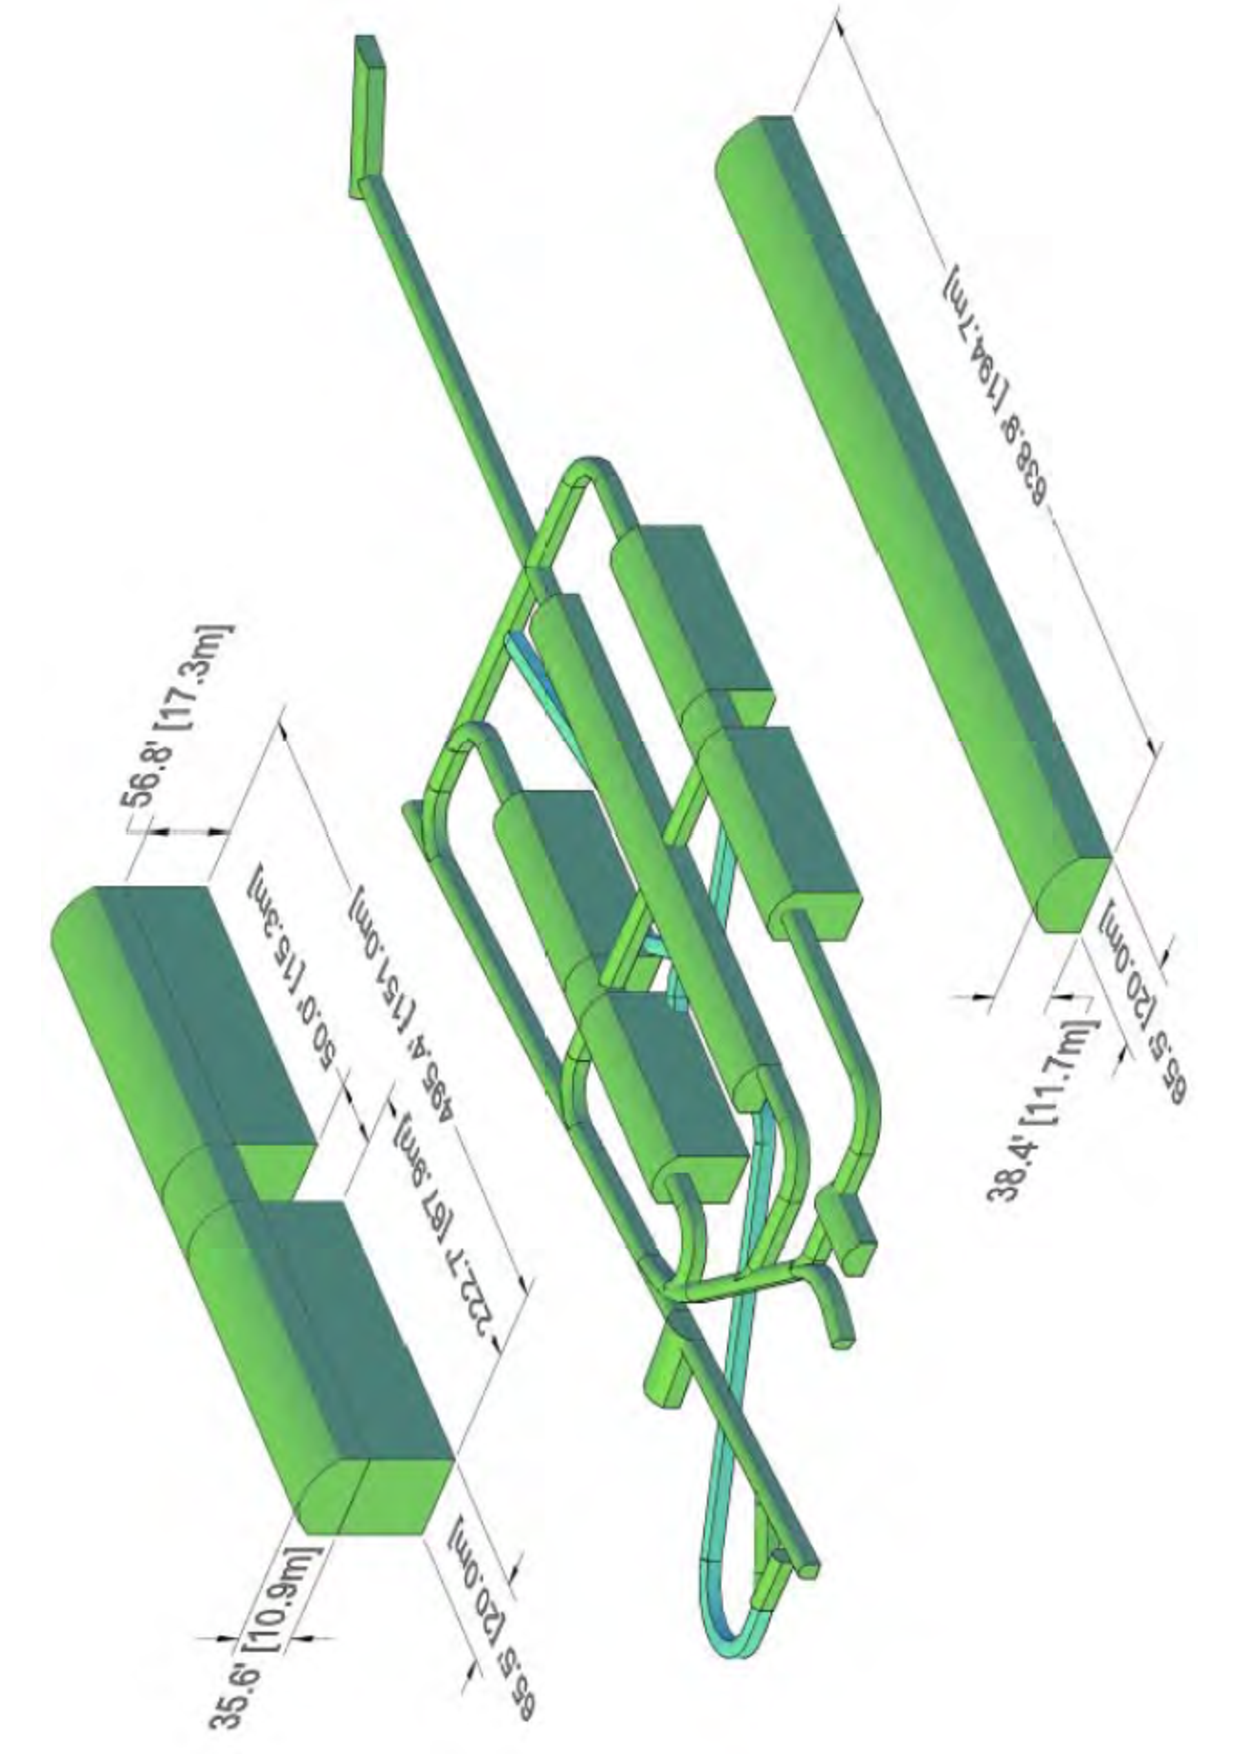
\includegraphics[width=0.7\textwidth]{DUNECavernSystem}
  \caption[A representation of the future LBNF cavern system at SURF]
          {A representation of the future LBNF cavern system at SURF. The top of the figure shows one of the main caverns, composed of two detector pits. The centre of the figure shows the entire cavern system, whilst the bottom of the figure shows area which will house the cryogenic equipment. All caverns shown need to be excavated. The Ross Shaft is located a small distance from the bottom left corner of the figure. The Yates Shaft is located roughly 1 km from the cavern system, in the direction of the top left hand corner of the figure. The dimensions shown are estimations, and the final dimensions may be slightly smaller. The figure is taken from~\citep{DUNECDR_V3}.}
  \label{fig:DUNECavernSystem}
\end{figure}

The other remit of LBNF is the design, and construction, of the beam line, as well as providing the facilities to house the DUNE ND. A schematic showing the near site facilities which will be built by LBNF is shown in Figure~\ref{fig:DUNENearDetectorComplex}. From Figure~\ref{fig:DUNENearDetectorComplex}, it can be seen that upon extraction from the Main Injector, the proton beam will be sent through a man-made embankment, the height of which will be approximately 18 m. This proton beam will then be bent 7.2$^{\circ}$ westward, and 5.8$^{\circ}$ downwards, so as to point towards the FD location at SURF. After being pointed towards SURF, the protons will hit a graphite target, producing mesons which will then be focused by a set of magnetic horns, before being passed to a 'decay pipe' where they decay to muons and neutrinos. The magnetic horns are able to 'sign select' the mesons produced by the interactions with the target, so as to only focus mesons which will decay into either neutrinos, or antineutrinos. This allows the beam produced by LBNF to operate in either neutrino or antineutrino mode, by focusing either positive, or negatively charged mesons, respectively. The energies of the neutrinos produced by the meson decays are between 0.5 and 5 GeV, this allows for a wide band neutrino beam to be used. The advantage of using a wide band neutrino beam is that the DUNE FD can then observe the maxima from the both the first, and second, oscillation maxima, at approximately 2.4 GeV, and 0.8 GeV, respectively. The reference design for the 'decay pipe' is 194 m long and filled with Helium. Studies are on-going to determine the most optimal separation of the beam-horns, and the most optimal length of the decay pipe~\citep{DUNECDR_V2, DUNECDR_V3}. At the end of the 'decay pipe' is an 'absorber' which will absorb any protons which did not interact with the target, and any mesons which have not decayed. \\

\begin{figure}
  \centering
  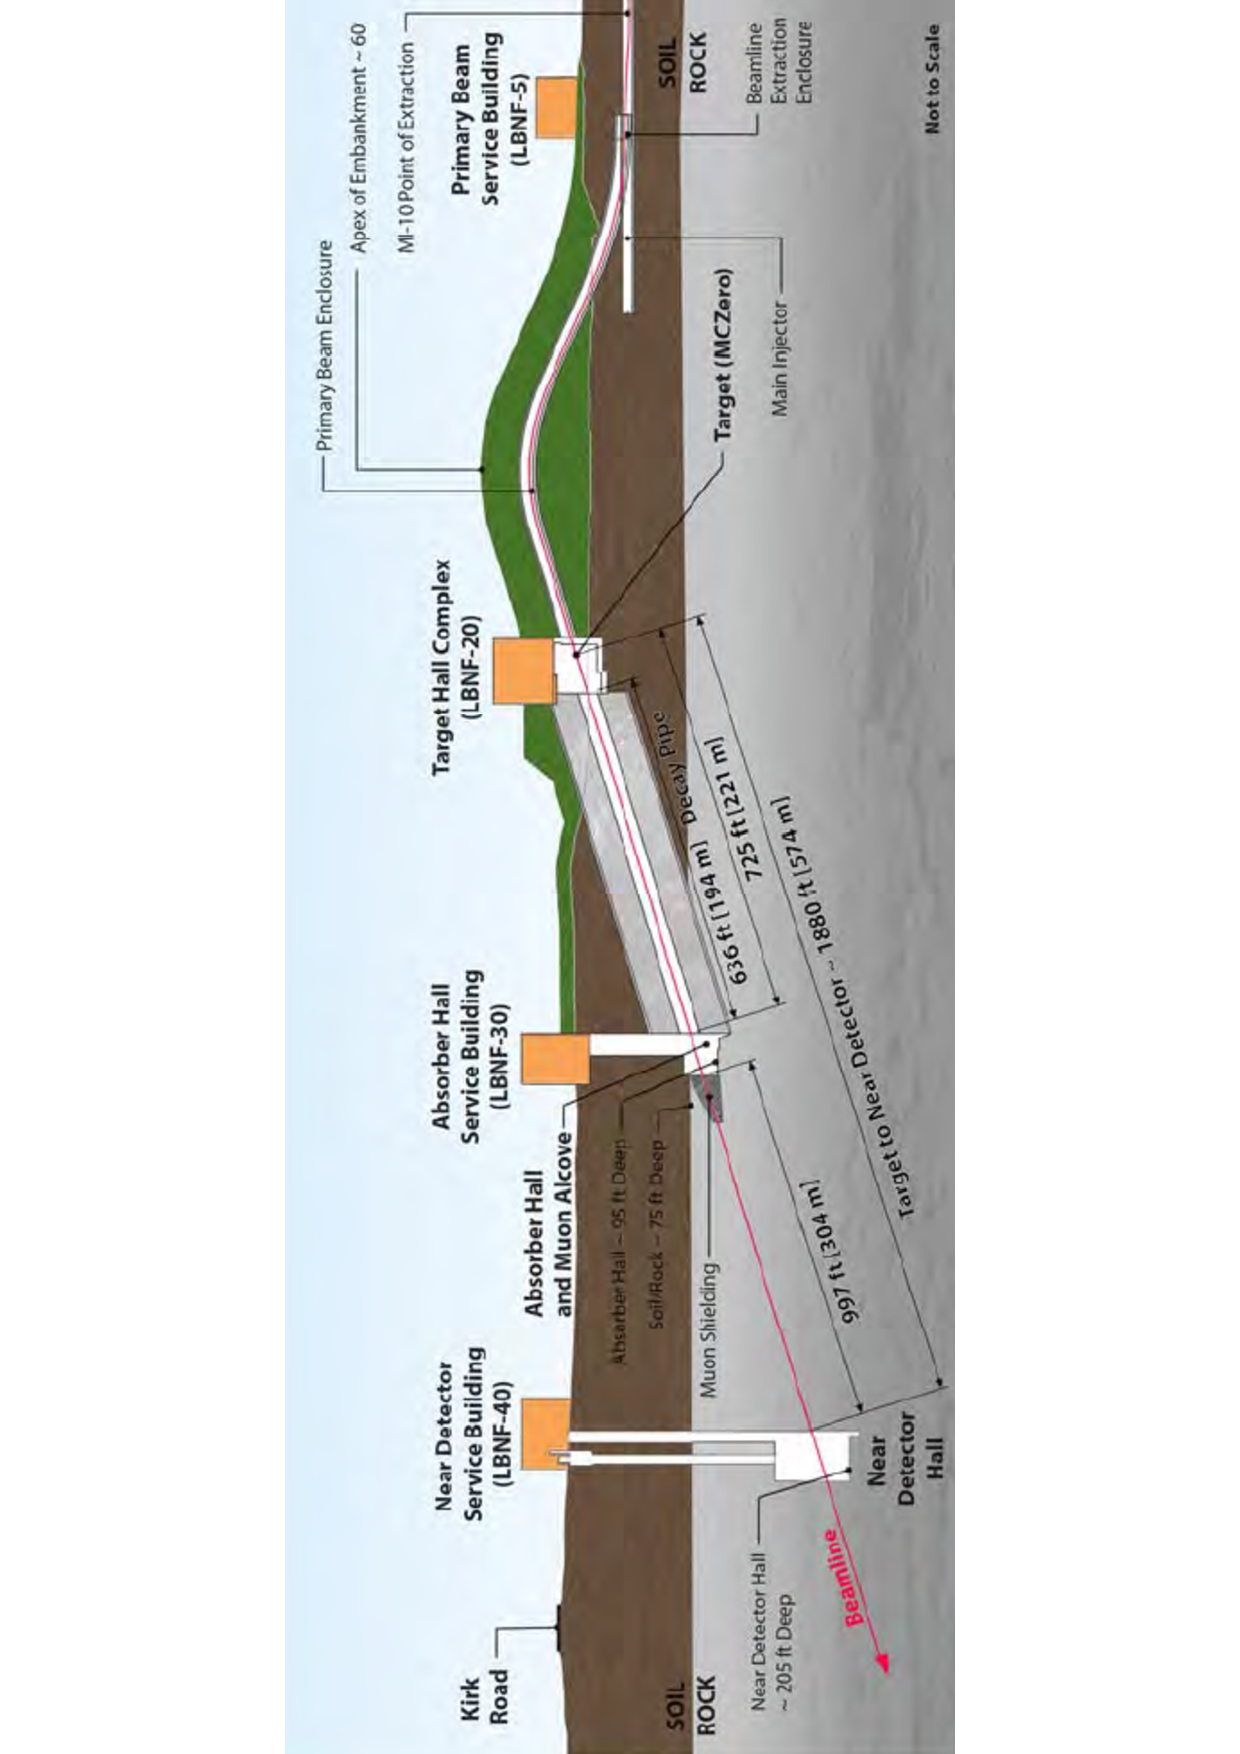
\includegraphics[width=0.9\textwidth]{NearDetectorComplex}
  \caption[A representation of the future LBNF near site at Fermilab]
          {A representation of the future LBNF near site at Fermilab. From right to left, the beam extraction point, man-made hill, target hall complex, meson decay pipe, absorber hall, and the near detector hall can be seen. Measurements are shown for the decay pipe (a reference design, top, and an alternative design, bottom), and the distance between the absorber hall and near detector are shown, though the figure is not to scale. All facilities need to built, including the extraction point from the Main Injector, and the man-made hill. The figure is taken from~\citep{DUNECDR_V3}.}
  \label{fig:DUNENearDetectorComplex}
\end{figure}

The beamline illustrated above will utilise the Main Injector beamline after the PIP-II upgrade~\citep{PIP-II}, whereby protons will be delivered with energies between 60 and 120 GeV, corresponding to a beam power of 1.0 to 1.2 MW. The ability to vary the beam power will give DUNE the ability to optimise the flux spectrum, and to better understand the systematic effects of the beam~\citep{DUNECDR_V1}. \\

Also associated with the near site is the construction of the DUNE ND. The distance between the ND and the absorber hall will be a minimum of 210 m, due to the muon-range-out distance, and is 304 m in the reference design~\citep{DUNECDR_V3}. The DUNE ND will be comprised of at least one detector, the exact details of the ND are covered in Section~\ref{sec:DUNEDetector_Near}. \\

%********************************** %Second Section  *************************************
\section{The potential DUNE Detector designs} \label{sec:DUNEDetector} %Section - X.3
Though all four FD modules will be LArTPCs, it has not been decided whether they will use a single (liquid) phase design, or a dual phase (liquid/gas) design. This is not true for the first 10 kt module, which will use a single phase design. The single phase design is outlined in Section~\ref{sec:DUNEDetector_SP}. Though this thesis concentrates on the single phase design, the dual phase design is also outlined in Section~\ref{sec:DUNEDetector_DP} for completeness. Similarly, though little mention will be made concerning the DUNE near detector, the reference design for the DUNE ND is outlined in Section~\ref{sec:DUNEDetector_Near}. These sections only present a relatively brief overview of the potential designs, for more detailed descriptions see~\citep{DUNECDR_V4}. \\

\subsection{The single phase detector design} \label{sec:DUNEDetector_SP}
In the single phase design, the charge generation, electron drift, and charge collection, all occur in the LAr. As the charge collection occurs in the LAr, this means that all of the TPC structure, including the electronics, have to be submerged. The fiducial volume of 10 kt, measuring 12 m high, 14.5 m wide (in the drift direction), and 58 m long (in the beam direction), is too big to be contained in a single TPC, and so many individual TPCs are required. The reason for this, is that it is not practical to collect electrons after they drift this far, or to construct an Anode Plane Assembly (APA) frame, and Cathode Plane Assembly (CPA) frame, which could accommodate this. There is also the added complication that the APA and CPA frames would have to be transported underground, and the mine shafts would not be able to accommodate frames this large. \\

Therefore, the active volume is separated into many TPCs, each produced by applying voltages to planes of APAs and CPAs. These planes of APAs and CPAs are enclosed by a field cage, constructed of FR4 Printed Circuit Board(PCB). In total there are 3 planes of APAs and 2 planes of CPAs, ordered such that there is a CPA plane in between any two APA planes, and there are APA planes on the outer faces of the detector. The separation of the APA and CPA planes is 3.6 m, with the ionised electrons drifting towards the APA planes, in an electric field of 500 V cm$^{-1}$. This means that the maximum drift length of the electrons is 3.6 m. The APA and CPA planes are orientated vertically, parallel to the beamline. Each plane of APAs contains 25 sets of APA rows, where each APA row contains two APA frames, stacked on top of each other. Each APA frame is 6 m high, and 2.3 m wide, meaning that two stacked APA frames give the total active volume height of 12 m. The 25 sets of 2.3 m wide APA frames, produce the total active volume in the beam direction of 58 m, after a small separation between APA rows is accounted for. The CPA planes are structured in an identical fashion, though each CPA frame is only 3 m high, therefore each CPA row contains 4 CPA frames. This results in there being a total of 150 APA frames, and 200 CPA frames in a given 10 kt module. Figure~\ref{fig:DUNE_SP_Schem}, shows a graphical representation of this APA and CPA frame structure, where in reality there would be an additional 24 planes, going into the page, identical to the one shown. \\

\begin{figure}
  \centering
  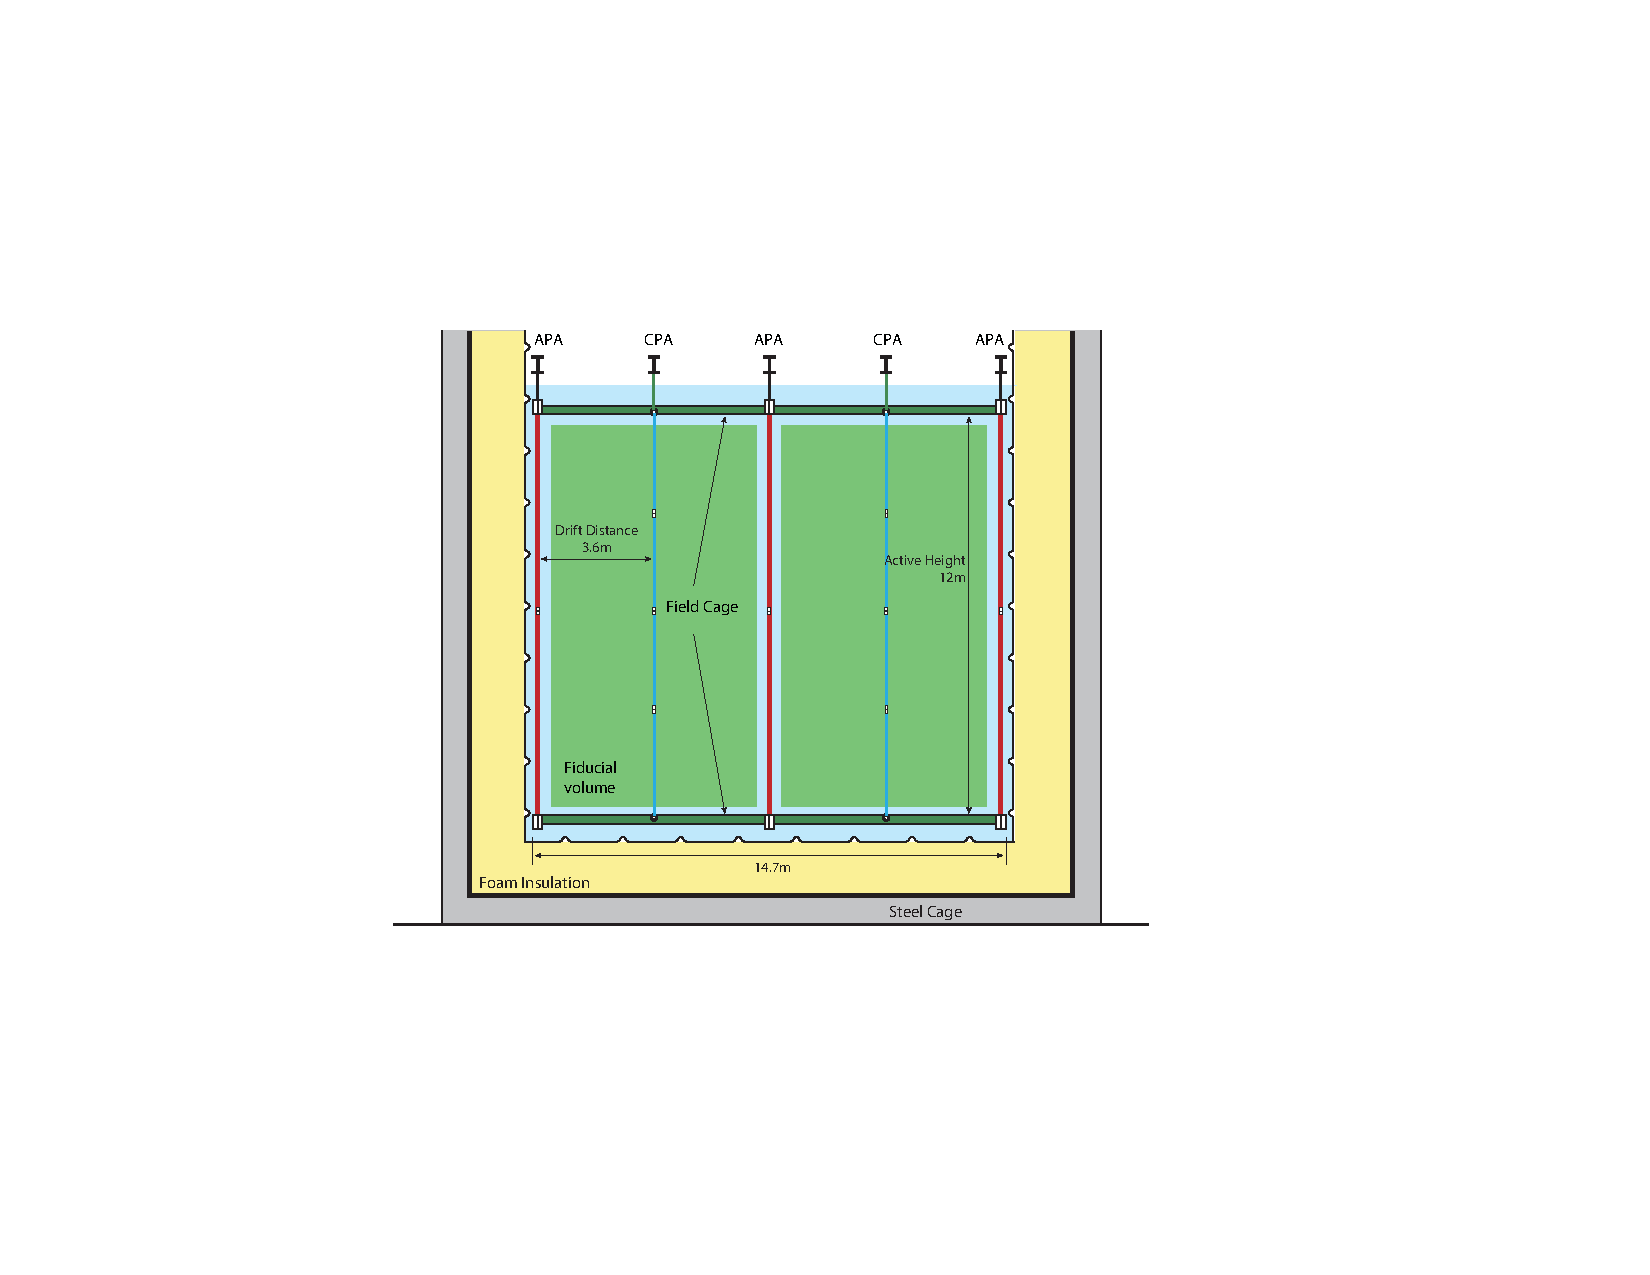
\includegraphics[width=0.7\textwidth]{SinglePhase_CrossSec}
  \caption[A cross section of the DUNE single phase detector design]
          {A cross section of the DUNE signal phase detector design. The plane shown is looking along the beamline, such that the detector extends a total of 58 m into the page. Planes of APAs (purple) and CPAs (blue) are shown on top of the fiducial volume (green), inside the foam insulation (yellow), which is further contained in the concrete (black line) and steel cage (grey) structures. A supporting structure, holding the APAs and CPAs is also shown (dark green). The boundaries between APA (CPA) frames are shown as black squares, such that each APA (CPA) plane contains 2 APA (4 CPA) frames.}
  \label{fig:DUNE_SP_Schem}
\end{figure}

Each APA frame is instrumented on both sides with 4 wires planes, the properties of which are outlined in Table~\ref{tab:DUNE_SP_WP}. The induction plane wires are wrapped around the long edges of the APA frames. This means that on each APA frame there are two sets of grid and collection planes, one on each side of the APA, and two induction plane wires, both of which are sensitive to both sides of the APA. The two induction planes are wrapped around the long edge of the APA frame, so that readout electronics are only required at one of the short ends of the APA frames. The electronics for the APAs at the top (base) of the detector, are placed on the edge of the APA frame which is closest to the top (base) of the detector. The electronics are outside of the active volume, but still submerged in the LAr. Though the induction plane wires are sensitive to particles in two different TPCS, the wire pitch is chosen such that there is no degeneracy between pairs of induction and collection wire pairs. The wire planes are biased such that the electrons will drift past the first three wire planes, and will be collected on the collection plane. An illustration of the wire wrapping is shown in Figure~\ref{fig:WirePitches}, where it is presented in the context of resolving degeneracy's between induction and collection plane wires. It is presented in this way because the 35 ton prototype, which is discussed in Section~\ref{sec:The35tonDetector}, had degeneracy's between the induction and collection plane wires, due to the wire pitches being different from the FD reference design. \\

\begin{table}
  \caption[The parameters of the wire planes in the DUNE FD single phase design]
          {The parameters of the wire planes in the DUNE FD single phase design.}
  \label{tab:DUNE_SP_WP}
  \centering
  \begin{tabular}{l c c c c}
    \toprule
    {Function}             & {Orientation ($^{\circ}$)} & {Pitch (mm)} & Num. Wires & Bias Voltage (V) \\ 
    \midrule
    Grid (G)               & 0                          & 4.79         & 960        & -655 \\
    
    1$^{st}$ induction (U) & 35.7                       & 4.67         & 800        & -365 \\
    
    2$^{nd}$ induction (V) & -35.7                      & 4.67         & 800        & 0    \\
    
    Collection (Z)         & 0                          & 4.79         & 960        & 860 \\
    \bottomrule
  \end{tabular}
\end{table}

\begin{figure}
  \centering
  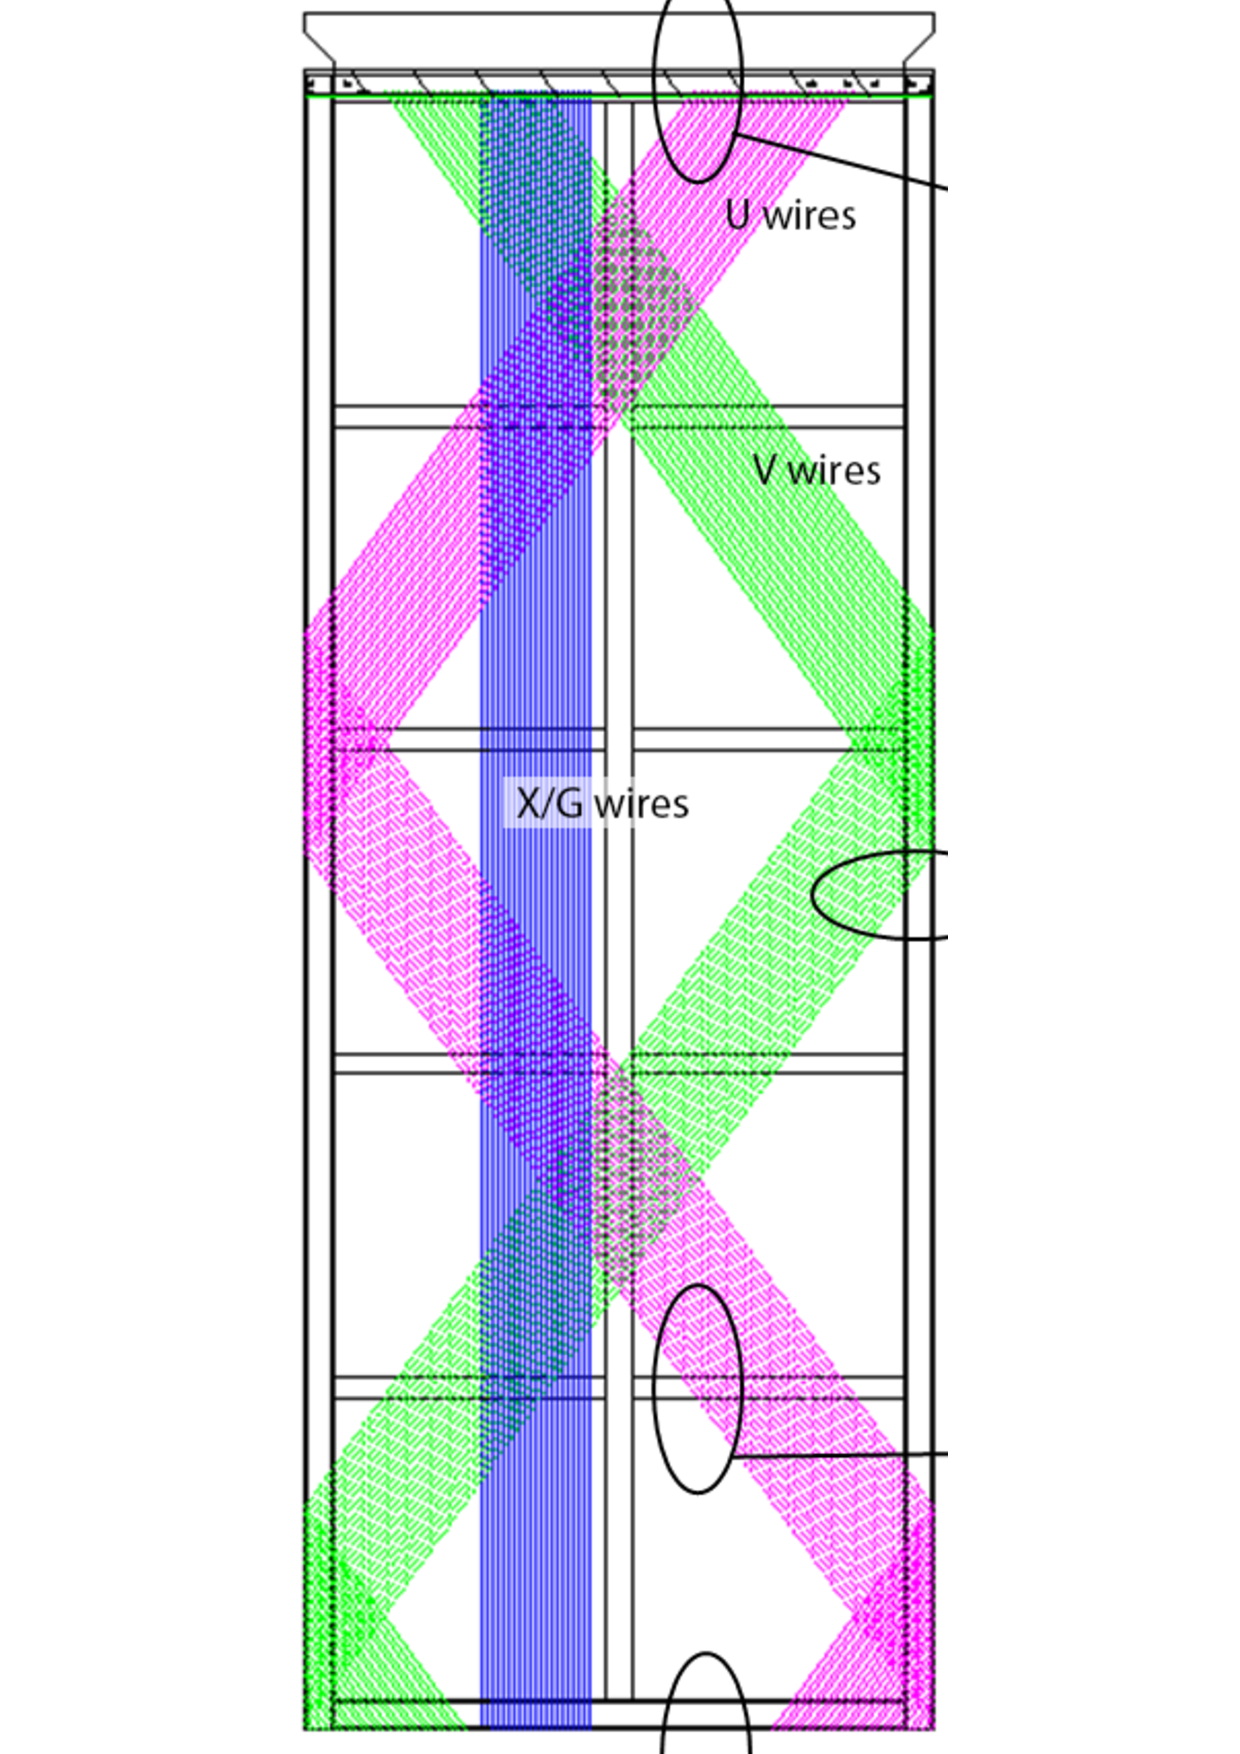
\includegraphics[width=0.3\textwidth]{tpc_apa_cross_sections}
  \caption[An illustration of the wire wrapping in the DUNE single phase design]
          {An illustration of the wire wrapping in the DUNE single phase design. A small number of the wires in each plane are shown. The wire planes shown, in the order that the electrons drift past them, are shown as follows; the 1$^{st}$ induction plane (U) is magenta, the 2$^{nd}$ induction plane (V) is green, and the collection plane (Z) is blue. The grid plane, which is in front of the 1$^{st}$ induction plane is parallel to the collection plane. The figure is taken from~\citep{DUNECDR_V4}.}  
  \label{fig:35tonWireGeom}
\end{figure}

It is also envisioned that there will be a system of Photon Detectors (PDs), to measure interaction times of both beam, and non-beam, events. An individual PD will be comprised of a light guide, and 12 Silicon Photo Multipliers (SiPMs). Each APA frame will contain 10 equally spaced PDs. The PDs will use a wavelength shifter on the surface of the light guide, to convert the 128 nm scintillation photons from the LAr, to photons with a wavelength of 430 nm. This wavelength shifted light will be collected by the SiPMs. The front end electronics for the SiPMs will reside outside of the cryostat, where a SiPM Signal Processor (SSP) digitises the signals from the SiPMs. \\

\subsection{The dual phase detector design} \label{sec:DUNEDetector_DP}
In the dual phase detector design the electrons are not collected in the LAr, but are extracted at the interface between liquid and gaseous argon, before being amplified, and collected, in the gaseous argon. This design follows the GLACIER concept\citep{GLACIER}, whereby the electrons are drifted vertically, before being collected by a finely segmented anode~\citep{1748-0221-8-04-P04012, 1748-0221-7-08-P08026, Badertscher:2010zg}. The amplification of electrons at the liquid/gas boundary is done using Large Electron Multipliers (LEMs). As a result of amplifying the drifted electrons the $signal/noise$ ratio can be increased by at least an order of magnitude. It also allows the threshold for measuring energy depositions to be lowered. \\

The dual phase design also has a larger fiducial volume, as there are no inactive regions in the LAr. This is because there are no gaps between the modules which read out the charge, called Charge Readout Planes (CRPs). The CRPs measure 3 $\times$ 3 m$^2$, and are composed of 36 LEM/Anode Sandwiches (LAS) modules which each measure 0.5 $\times$ 5 m$^2$. The LAS modules, are themselves composed of an anode and a LEM, both measuring 0.5 $\times$ 5 m$^2$. The process by which charge is read out, is as follows; the drifted electrons are first extracted by a grid plane, submerged in the LAr by comb-teeth blades, which is made of wires with a separation of 3.125 mm. After extraction, done by applying an electric field of the order of 2 kV cm$^{-1}$, the electrons pass through the LEMs. The LEMs have a honeycombed structure of 500 $\mu$m holes, with a separation of 800$\mu$m, giving a total of around 200 holes per cm$^2$. An electric field of the order 30 kV cm$^{-1}$ is applied between the electrodes of the LEMs, causing large avalanches, this is how large $signal/noise$ ratios can be measured. These electrons then experience a field of roughly 5 kV cm$^{-1}$, before finally being collected at the anodes. The anodes are composed of a pattern of gold plated copper tracks, on a single multi-layered PCB, the layout of which is composed such that both $x$ and $y$ views collect the same amount of charge, independent of track angle. The CRPs are produced by attaching LAS modules together, which are then further attached to the grid planes. Figure~\ref{fig:DUNE_DP_Schem} is an illustration showing the charge collection process in the dual phase design. \\

\begin{figure}
  \centering
  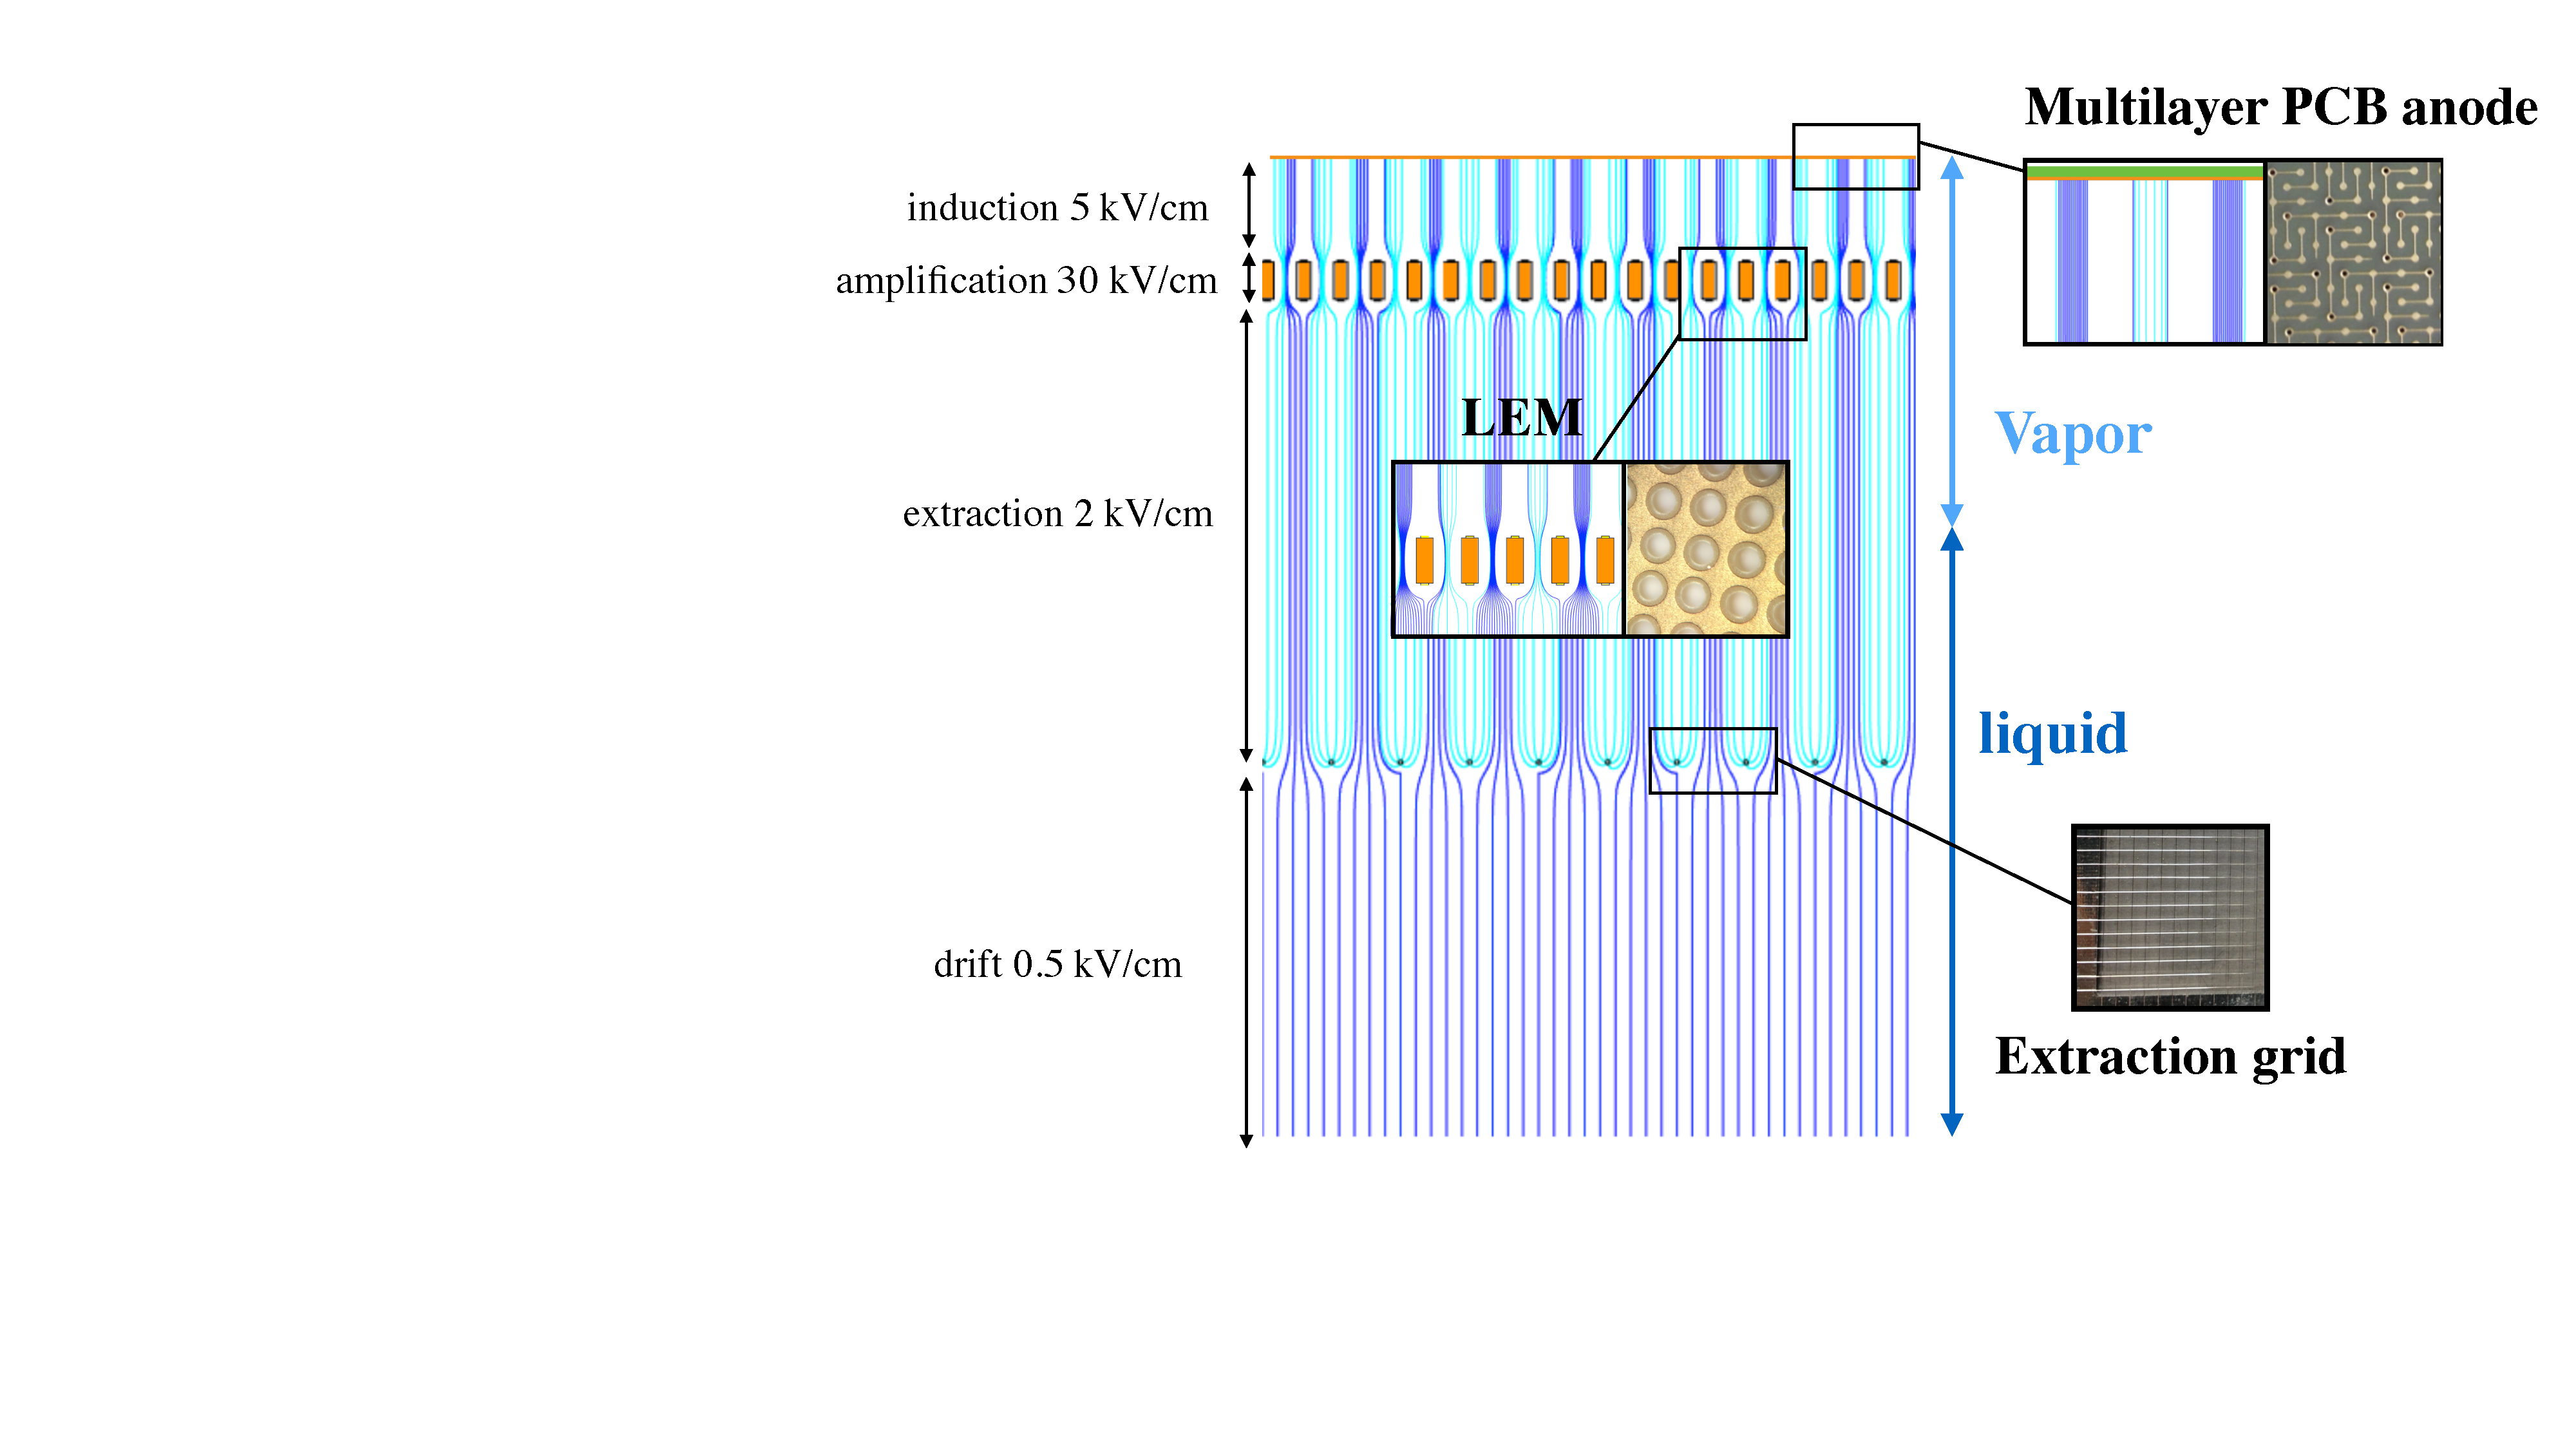
\includegraphics[width=0.85\textwidth]{DualPhasePrinciple}
  \caption[An illustration of the process of charge extraction in the DUNE dual phase detector design]
          {An illustration of the process of charge extraction in the DUNE dual phase detector design. The liquid/gas boundary can be seen to be between the grid plane and the LEMs. The various electric fields which electrons experience at the different stages of extraction can be seen, as well as small pictorial representations of the various instruments used in the extraction process. The figure is taken from~\citep{DUNECDR_V4}.}
  \label{fig:DUNE_DP_Schem}
\end{figure}

As was the case with the single phase design, the dual phase detector design contains a system to collect the scintillation light. However, in the dual phase design, this will be done using 8-inch Photo Multiplier Tubes (PMTs), coated with TPB, which are located about 1 m below the cathode. The use of PMTs like this have been used extensively in giant water Cherenkov detectors, and so it is envisioned that many of the techniques used there will be utilised~\citep{1748-0221-6-01-C01081, Genolini:2008uc}. \\ 

\subsection{Reference near detector design} \label{sec:DUNEDetector_Near}
The reference DUNE ND is a Fine-Grained Tracker (FGT), which consists of a Straw-Tube Tracking (STT) module, and an Electromagnetic Calorimeter (ECal), inside a 0.4 T dipole magnet. This is a design which builds on existing ND systems in experiments such as MINOS, NO$\nu$A, and T2K, as well as the NOMAD detector at CERN. The DUNE ND will also have a set of muon identifiers in the dipole magnet. A detector of this structure will allow the DUNE ND to make precision measurements of the neutrino flux, cross section, and the signal and background rates. A schematic of the potential ND system in DUNE is shown in Figure~\ref{fig:DUNE_Near_Schem}. \\

\begin{figure}
  \centering
  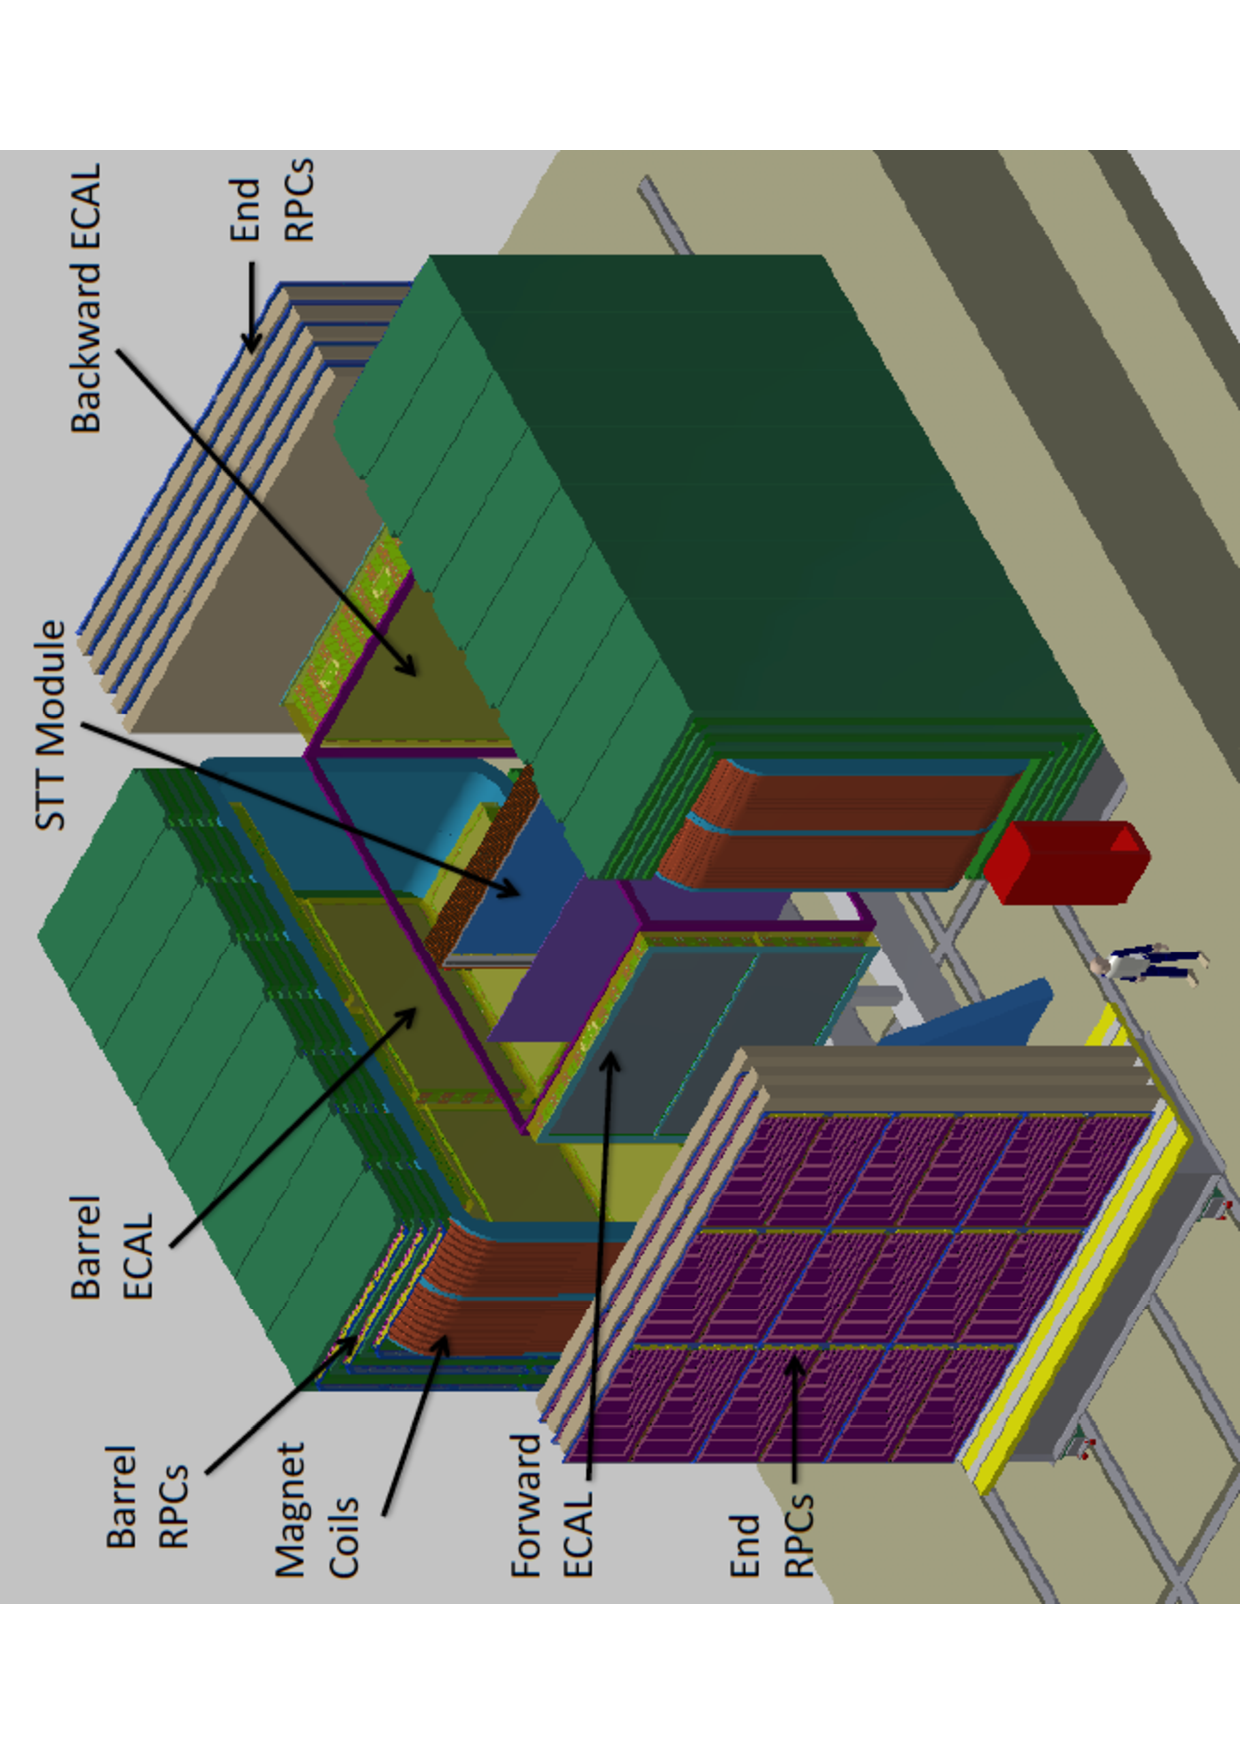
\includegraphics[width=0.65\textwidth]{STT_Schematic}
  \caption[A schematic representation of what the reference DUNE ND could look like]
          {A schematic representing of what the reference DUNE ND could look like. The main features of the detector, namely, the Straw-Tube Tracking (STT) modules, the Electromagnetic Calorimeter (ECAL), the Resistive Plate Chambers (RPCs) which make up the muon-identifiers, and the magnetic coils, can all be seen. The figure is taken from~\citep{DUNECDR_V4}.}
  \label{fig:DUNE_Near_Schem}
\end{figure}

There is also the possibility of building multiple NDs, to complement the FGT. One such potential ND would be a small ($\sim$100 ton) LArTPC. This would have the advantage of using the same technology as the DUNE FD, and so systematic effects could be better accounted for between the ND and FD. However, due to the slow drift time of LArTPCs, and the high luminosity of the beam, pile-up could become a problem. This is because there would be such a large number of neutrino interactions when the beam is operating at full power. The effect of pile-up would, however, be reduced when the beam is at running at low intensities such as, during the initial ramp-up, during periodic shut downs, or during upgrades to the beam. \\

%********************************** %Third Section  *************************************
\section{The physics capabilities of DUNE} \label{sec:DUNEPhys}%Section - X.2
As mentioned above, DUNE hopes to be able to deliver a wide ranging physics program. These topics include, but are not limited to, precision measurements of neutrino oscillation physics, discussed in Section~\ref{sec:DUNEPhys_Neut}, searching for nucleon decay in several important decay modes, discussed in Section~\ref{sec:DUNE_NDK}, and the detection and measurement of the $\nu_e$ flux from a core-collapse supernovae in our galaxy, should one occur, this is discussed in Section~\ref{sec:DUNE_Other}. \\

%********************************** % 3.1 Section  *************************************
\subsection{Neutrino physics} \label{sec:DUNEPhys_Neut} %Section - X.2.1
The primary goals of DUNE concern neutrino physics, many of these ideas were introduced in Section~\ref{sec:NeutPhys}. The primary goals of DUNE are outlined now, and illustrated more fully below~\citep{DUNECDR_V2}:
\begin{itemize}
\item Determine the neutrino mass hierarchy.
\item Measure the charge-parity (CP) violating phase - $\delta_{CP}$.
\item Make precision measurements of the neutrino mixing parameters, such as $\theta_{13}$, $\theta_{23}$, and $\Delta m^{2}_{31}$.
\end{itemize}
There are also secondary physics goals concerning neutrino physics, these include:
\begin{itemize}
\item Measuring the rate of $\nu_{\tau}$ appearance.
\item Measuring neutrino oscillations using atmospheric neutrinos.
\item Measuring a wide range of neutrino cross-sections, using the ND.
\item Measuring nuclear effects, particularly neutrino final-state interaction, using the ND.
\end{itemize}
Section~\ref{sec:DUNESched}, presented the idea of a staged approach to DUNE. As such, the annual exposure which DUNE is exposed to, will increase as a function of time. The exposure as a function of time is shown in Table~\ref{tab:DUNEExposure}, these exposures are important when considering the figures presented below. \\

\begin{table}
\caption[The exposure in units in units of kt MW years, as a function of time, assuming a staged DUNE construction]
        {The exposure in units in units of kt MW years, as a function of time, assuming a staged DUNE contraction. The table is taken from~\citep{Elizabeth_01_17}.}
\centering
\label{tab:DUNEExposure}
\begin{tabular}{c c}
\toprule
{Exposure (kt MW years)} & {Exposure (years)} \\
\midrule
171                      & 5 \\

300                      & 7 \\

556                      & 10 \\

984                      & 15 \\
\bottomrule
\end{tabular}
\end{table}

As presented in Section~\ref{sec:NeutPhys}, both the matter effect, and $\delta_{CP}$ introduce an asymmetry between neutrino and anti-neutrino oscillations. As the matter effect is caused by the difference in the presence/absence of electrons/positrons in the Earth, it increases with distance. The result of this is that for baselines longer than approximately 1000 km the two effects can be resolved~\citep{Bass:2013vcg}. It is for this reason that with a baseline of 1300 km, DUNE will be able to unambiguously determine the neutrino mass hierarchy, and determine $\delta_{CP}$~\citep{Diwan:2004bt}. \\

The reason for requiring a broadband neutrino beam can be seen in Figure~\ref{fig:DUNEOscillProb}, where it can be seen that whilst the energy of the first neutrino oscillation maxima is relatively unaffected by the value of $\delta_{CP}$, the energies of the higher oscillation maxima are strongly affected by the value of $\delta_{CP}$. The result of this, is that it is vital that DUNE is able to accurately the measure the rate of $\nu_e$ appearance at the lowest energies of the neutrino beam it receives from LBNF. It can also be seen that there are large differences in the expected oscillation probabilities for neutrinos and anti-neutrinos. Therefore, in order to measure the effect of $\delta_{CP}$, the beam from LBNF will also have to be able to operate in both neutrino and anti-neutrino mode. \\

\begin{figure}
  \centering 
  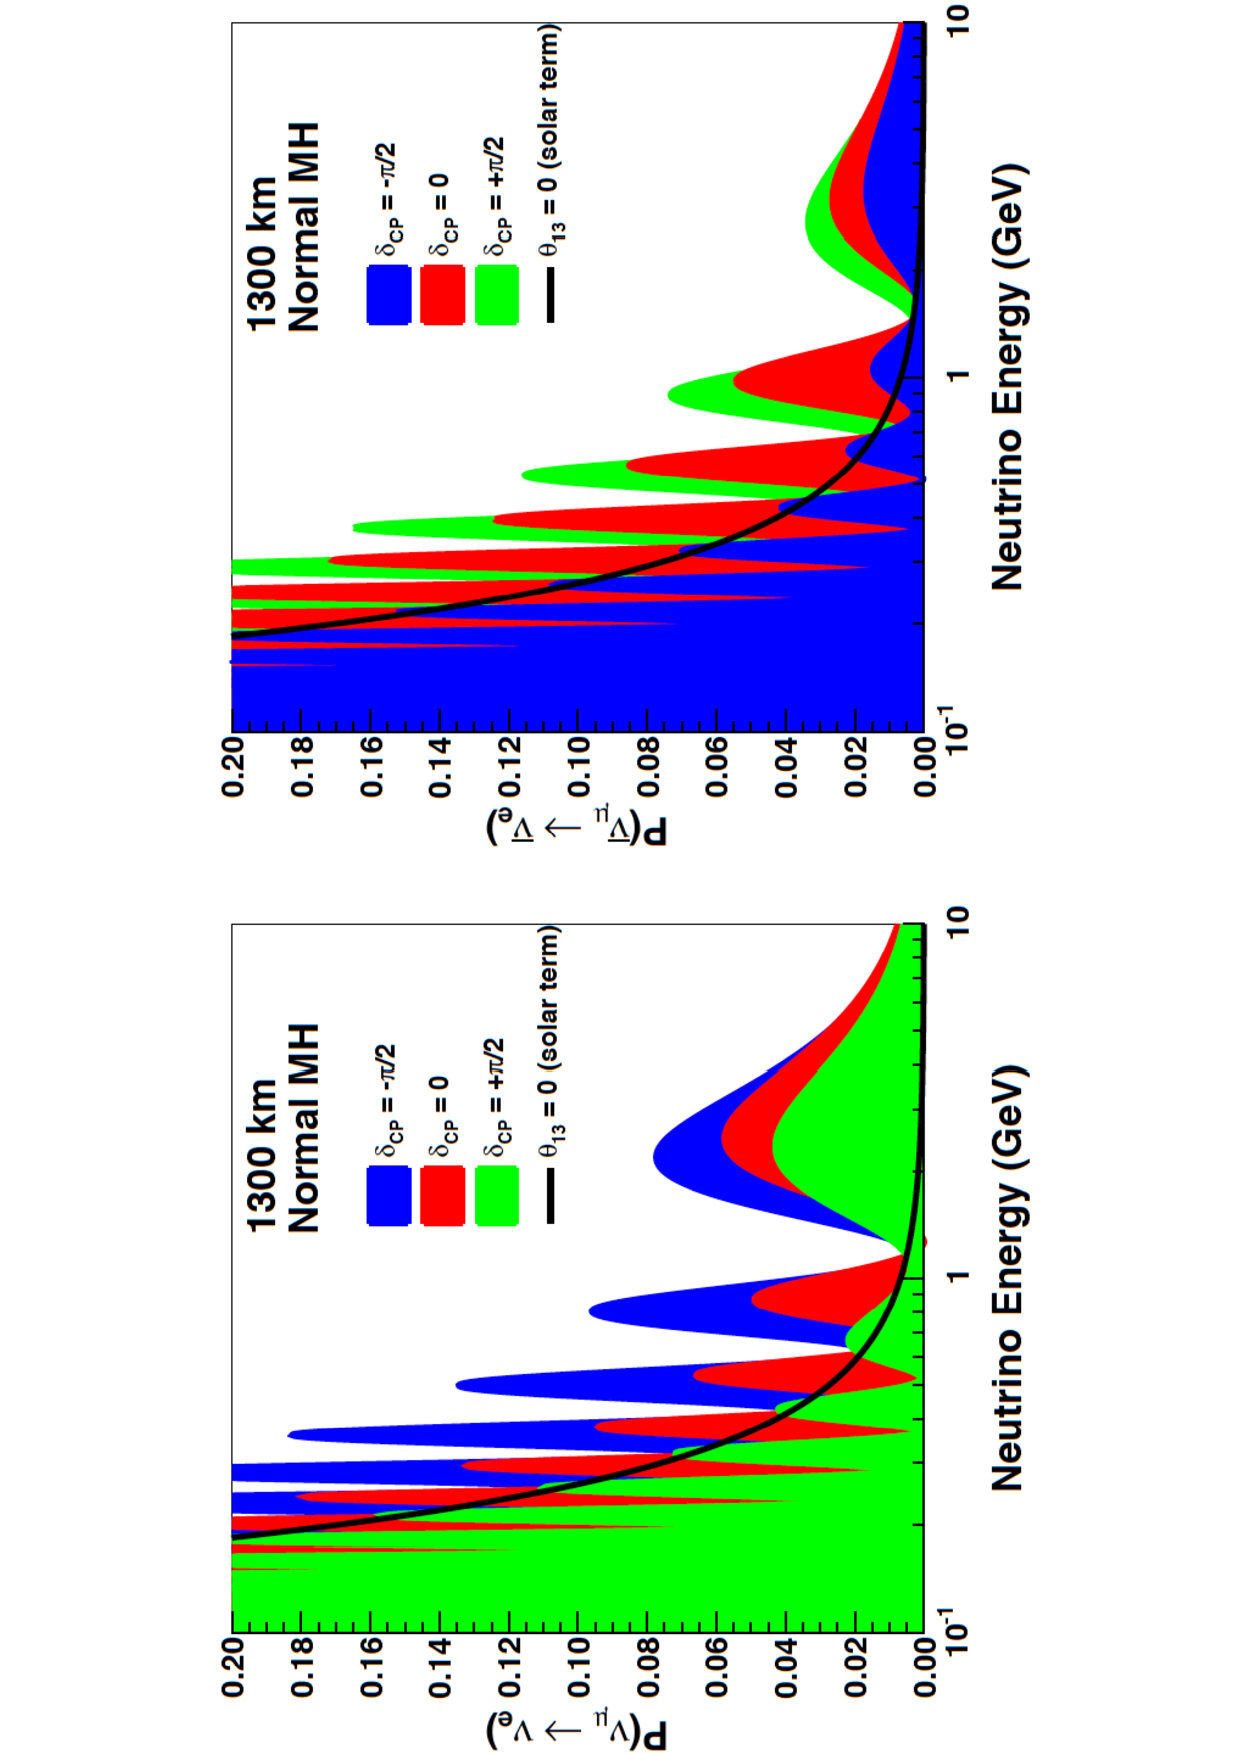
\includegraphics[width=0.9\textwidth]{DUNEOscillProb}
  \caption[The $\nu_e$ appearance probability at 1300 km as a function of neutrino energy, for a range of values of $\delta_{CP}$]
          {The $\nu_e$ appearance probability at 1300 km as a function of neutrino energy, for a range of values of $\delta_{CP}$. Left shows the probabilities for neutrinos, whilst right shows the probabilities for anti-neutrinos. Both figures assume normal mass hierarchy ($\nu_e$ is the lightest state). The probabilities for different values of $\delta_{CP}$ are shown, $\delta_{CP} = -\pi/2$ (blue), $\delta_{CP} = 0$ (red), $\delta_{CP} = \pi/2$ (green). The figure is taken from~\citep{DUNECDR_V2}.}
  \label{fig:DUNEOscillProb}
\end{figure}

When presenting the DUNE sensitivities to the determinations of the mass hierarchy, and the value of $\delta_{CP}$, figures are shown with exposures corresponding to 7 and 10 years worth of data taking~\citep{Elizabeth_01_17}. These exposures are calculated given the phased approach to DUNE which was outlined in Section~\ref{sec:DUNESched}. As such, 7 years of data corresponds to a beam exposure 300 kt MW yrs, whilst 10 years of data corresponds to a beam exposure of 556 kt MW yrs. The best fit values from NuFit 2016~\citep{NuFit2016} are used when making the figures, and equal running in neutrino and antineutrino mode is assumed. These figures are different to those presented in the DUNE CDR~\citep{DUNECDR_V2}, where only exposures of 300 kt MW yrs were shown. The figures taken from the CDR~\citep{DUNECDR_V2} show the effect that the two beam designs have on the sensitivities, whilst in the newer plots~\citep{DUNE2332, DUNE2335, DUNE2377, DUNE2401, DUNE2407} the optimised beam design is assumed. \\

Figure~\ref{fig:DUNEMassHierarchy} shows the significance with which DUNE will be able to determine the neutrino mass hierarchy, for all values of $\delta_{CP}$. It can be seen that the mass hierarchy can be determined with a significance of $\sqrt{\overline{\Delta{\chi^2}}}$ = 5, for all values of $\delta_{CP}$, after 7 years of data taking. It can also be seen that the mass hierarchy can be more conclusively determined if the hierarchy is inverted. \\

\begin{figure}
  \centering
  \begin{subfigure}{0.49\textwidth}
    \centering
    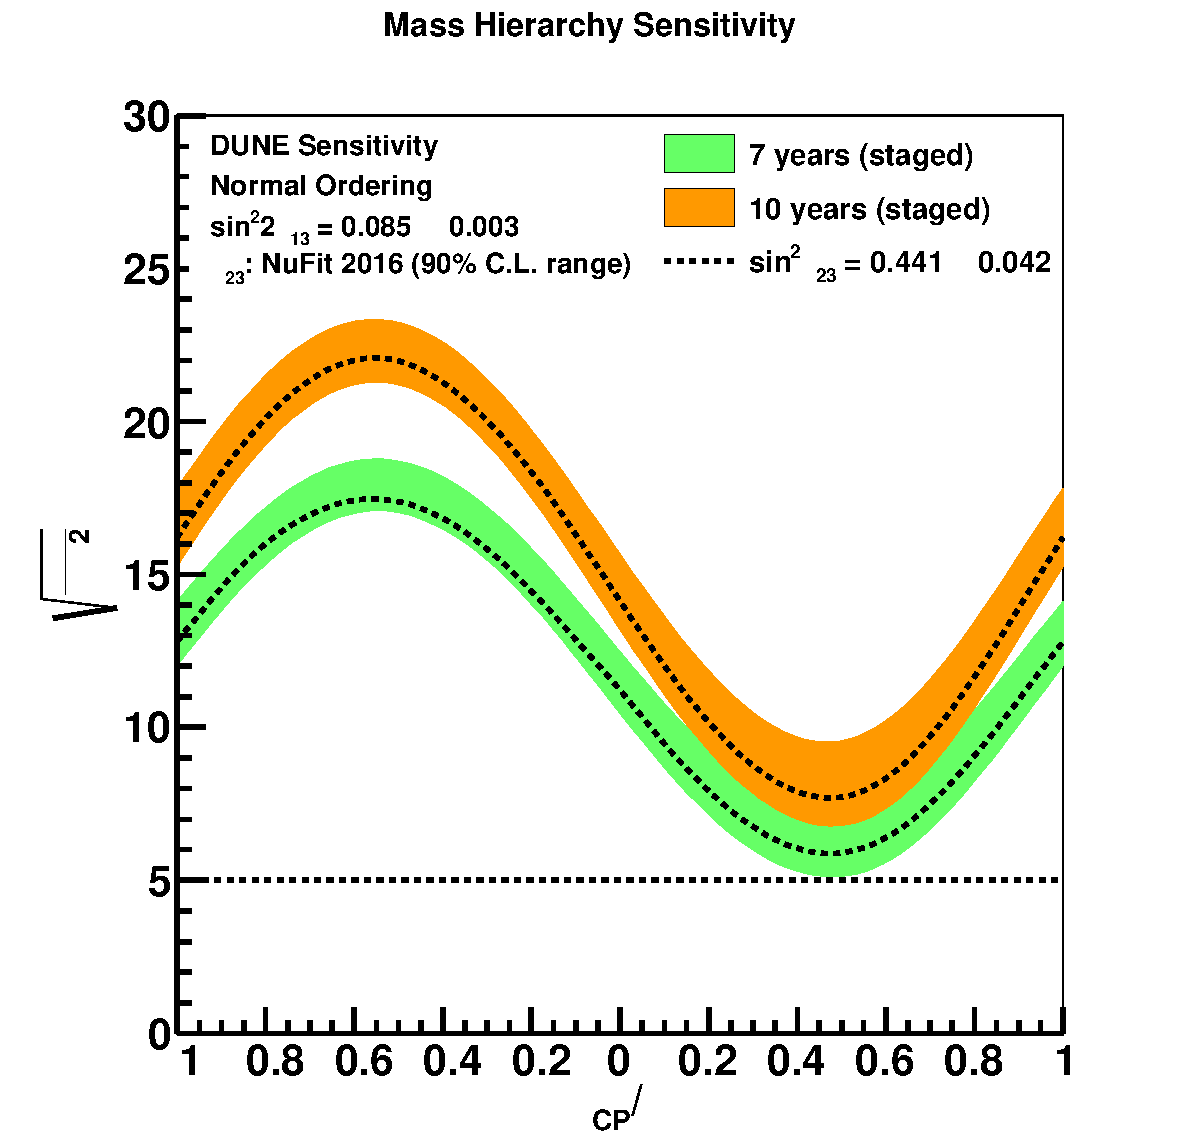
\includegraphics[width=\textwidth]{mh_two_exps_th23band_no_2017}
    \caption{Normal ordering.}
  \end{subfigure}%
  \begin{subfigure}{0.49\textwidth}
    \centering
    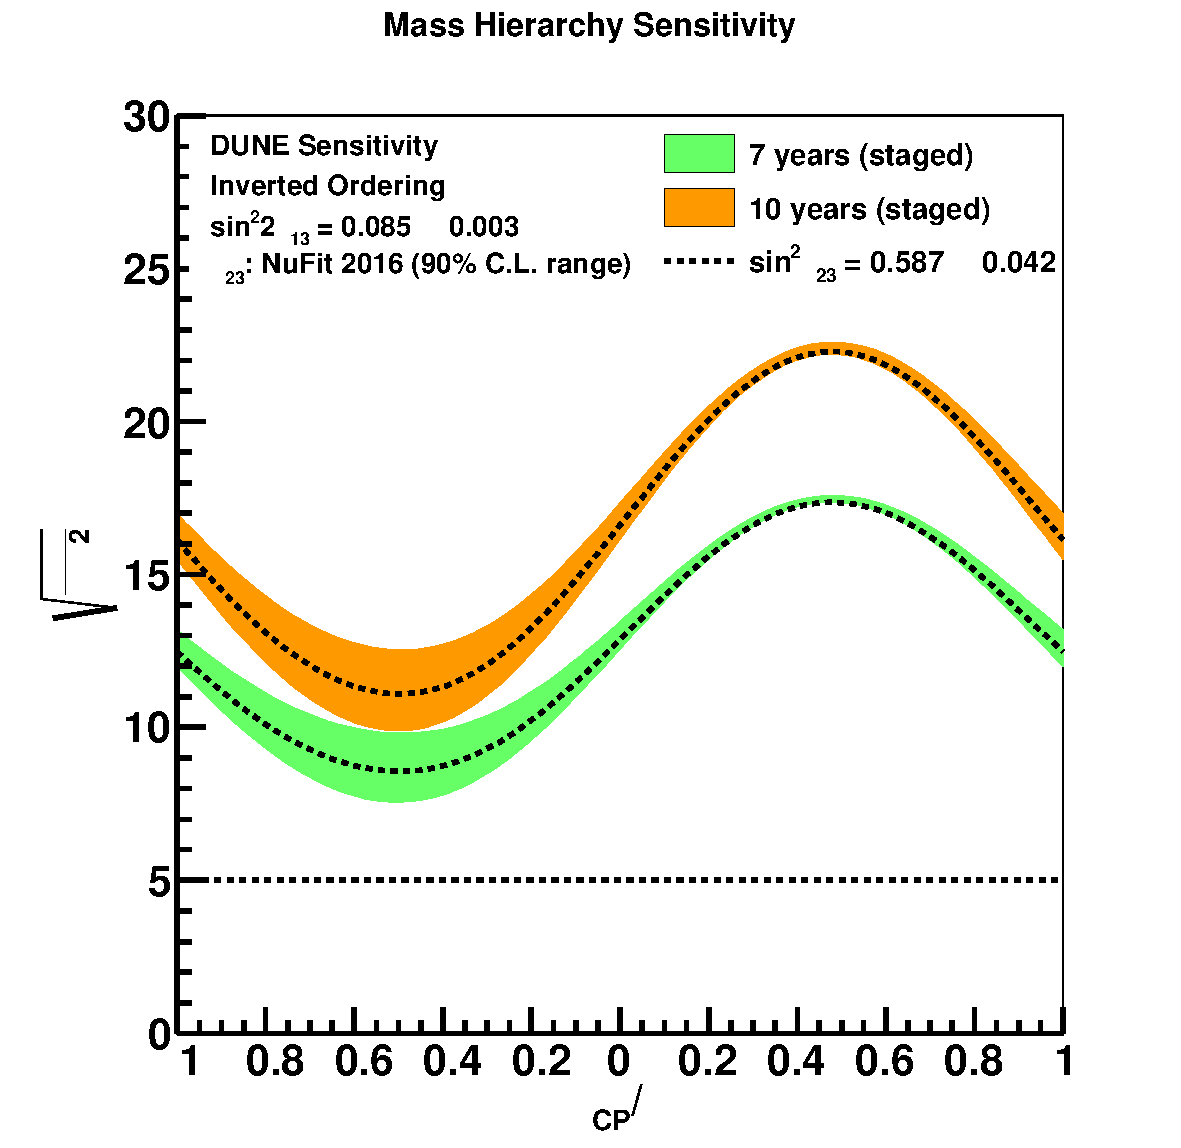
\includegraphics[width=\textwidth]{mh_two_exps_th23band_io_2017}
    \caption{Inverted ordering.}
  \end{subfigure}
  \caption[The significance with which DUNE will be able to determine the neutrino mass hierarchy, for all values of $\delta_{CP}$]
          {The significance with which DUNE will be able to determine the neutrino mass hierarchy, for all values of $\delta_{CP}$. Left shows the sensitivity assuming normal ordering, whilst right shows the sensitivities assuming inverted ordering. The shaded region shows the range of sensitivities for the 90\% confidence level range for $\theta_{23}$ values, the dashed line shows the sensitivity for the NuFit central value of $\theta_{23}$. The figure is taken from~\citep{DUNE2335}.}
  \label{fig:DUNEMassHierarchy}
\end{figure}

Figure~\ref{fig:DUNECPViolation} shows the significance with which DUNE will be able to determine the value of $\delta_{CP}$, for all values of $\delta_{CP}$. It can be seen that even with 10 years worth of data there are regions where the value of $\delta_{CP}$ cannot be determined accurately, this is because if $\delta_{CP}$ equals $-\pi$, 0, or $\pi$ there would be no CP-violation. Therefore, for values of $\delta_{CP}$ around these values, the significance to which $\delta_{CP}$ can be determined must approach 0. As such, even at very large exposures of over 800 kt MW yr, corresponding to around 13 years of data taking according to Table~\ref{tab:DUNEExposure}, only 75\% of the $\delta_{CP}$ values can be determined to a significance of 3$\sigma$, when using the optimised beam design~\citep{DUNE2401}. However, even with a relatively modest exposure of 150 (550) kt MW yr, DUNE can determine the value of $\delta_{CP}$ for over 50\% of the values for $\delta_{CP}$ to a significance of 3$\sigma$ (5$\sigma$) using the optimised beam design~\citep{DUNE2401}. This shows that should the value of $\delta_{CP}$ be close to a CP-conserving value, it would be very difficult to determine the value of $\delta_{CP}$. However, if it is far away from these values, DUNE could make a measurement, with a significance of over 5$\sigma$, in a matter of years. \\

\begin{figure}
  \centering
  \begin{subfigure}{0.49\textwidth}
    \centering
    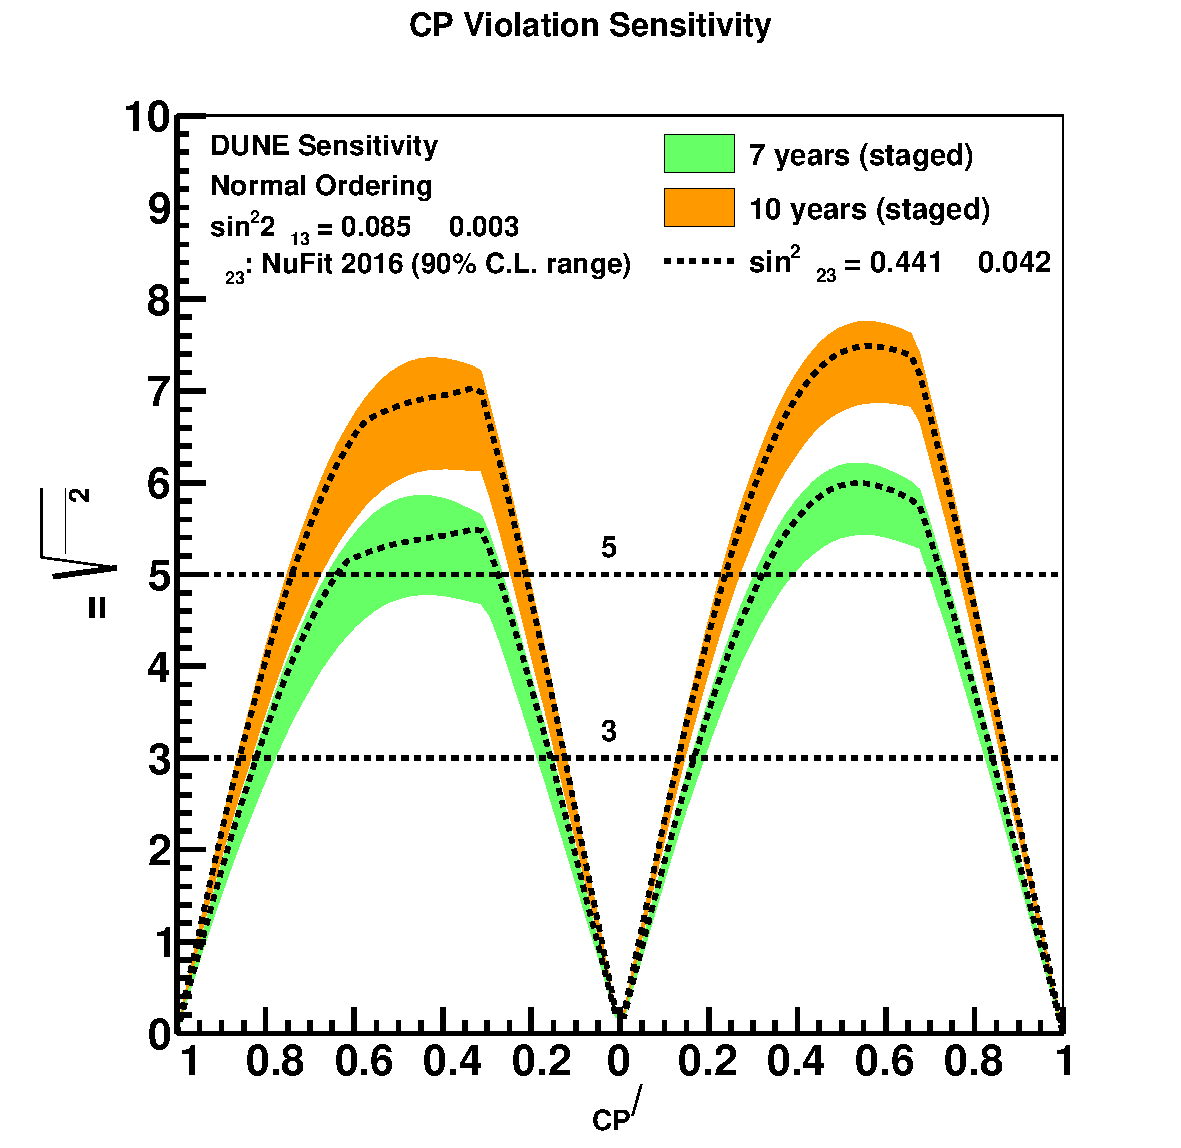
\includegraphics[width=\textwidth]{cpv_two_exps_th23band_no_2017}
    \caption{Normal ordering.}
  \end{subfigure}%
  \begin{subfigure}{0.49\textwidth}
    \centering
    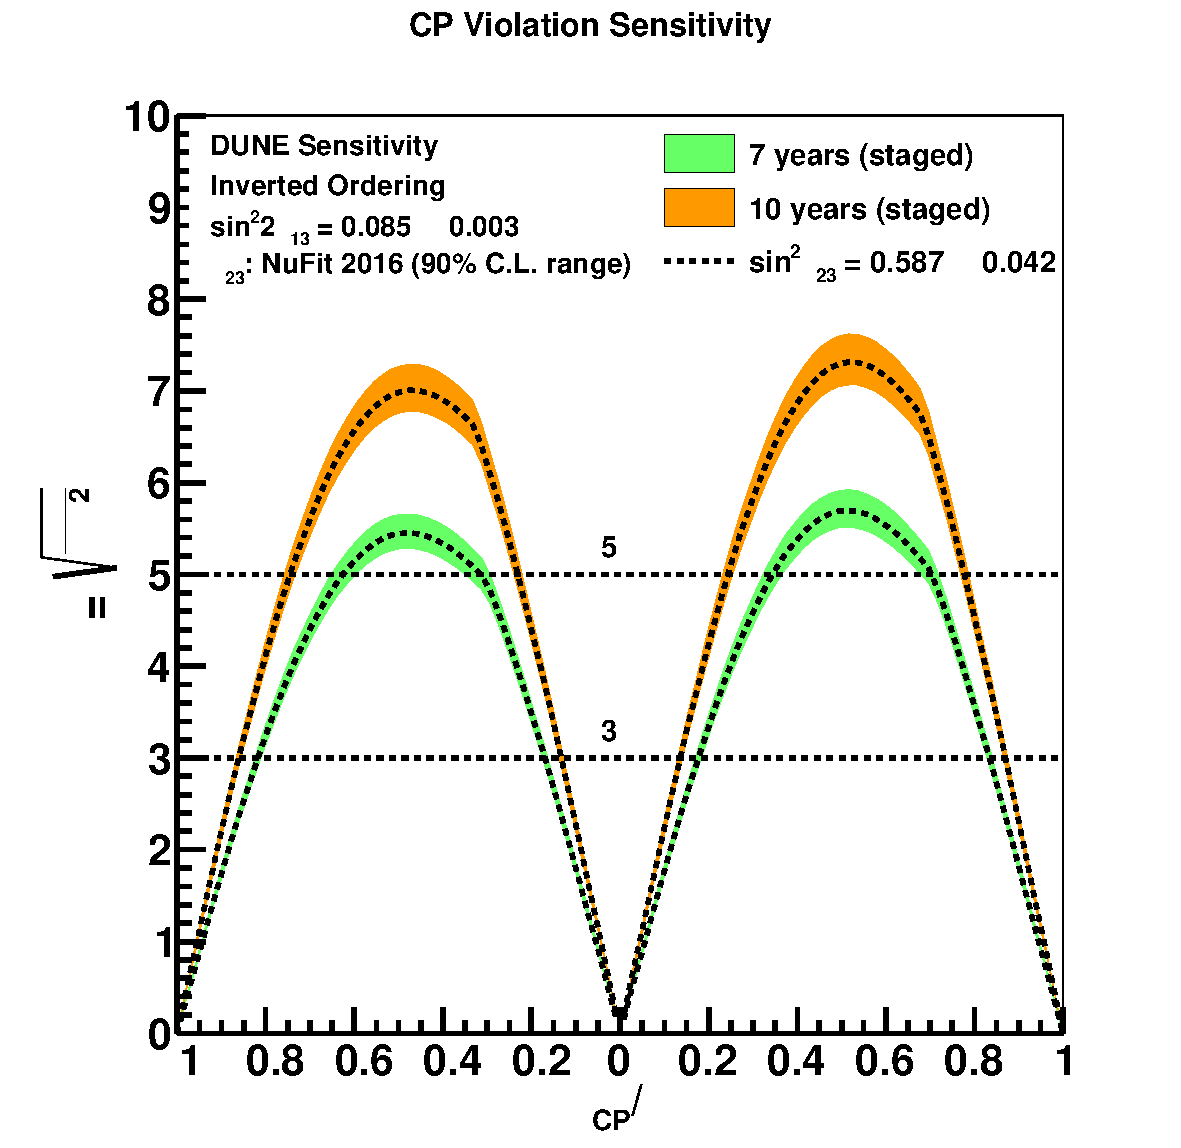
\includegraphics[width=\textwidth]{cpv_two_exps_th23band_io_2017}
    \caption{Inverted ordering.}
  \end{subfigure}
  \caption[The significance with which DUNE will be able to determine the value of $\delta_{CP}$, for all values of $\delta_{CP}$]
          {The significance with which DUNE will be able to determine the value of $\delta_{CP}$, for all values of $\delta_{CP}$. Left shows the sensitivity assuming the normal ordering, whilst right shows the sensitivities assuming inverted inverted. The shaded region shows the range of sensitivities for the 90\% confidence level range for $\theta_{23}$ values, the dashed line shows the sensitivity for the NuFit central value of $\theta_{23}$. The figure is taken from~\citep{DUNE2332}.}
  \label{fig:DUNECPViolation}
\end{figure}

Given the structure of Figure~\ref{fig:DUNECPViolation}, it can be instructive to instead observe the resolution to which the value of $\delta_{CP}$ can be determined with increasing exposures, this is shown in Figure~\ref{fig:DUNECPViolationRes}. Figure~\ref{fig:DUNECPViolationRes} shows curves for the cases when the value of $\delta_{CP}$ is both maximally CP-violating ($\delta_{CP}$ = 90$^{\circ}$), and when it is CP-conserving ($\delta_{CP}$ = 0$^{\circ}$). Somewhat paradoxically, the resolution is better when $\delta_{CP}$ = 0$^{\circ}$, the reason for this, is that the region of values of $\delta_{CP}$ for which CP-violation would not be observed, becomes increasingly small, as exposure increases. This means that the resolution to which $\delta_{CP}$ can be determined increases. However, the more interesting result, would be the one which supported $\delta_{CP}$ having a value which causes maximal CP-violation. \\

\begin{figure}
  \centering
  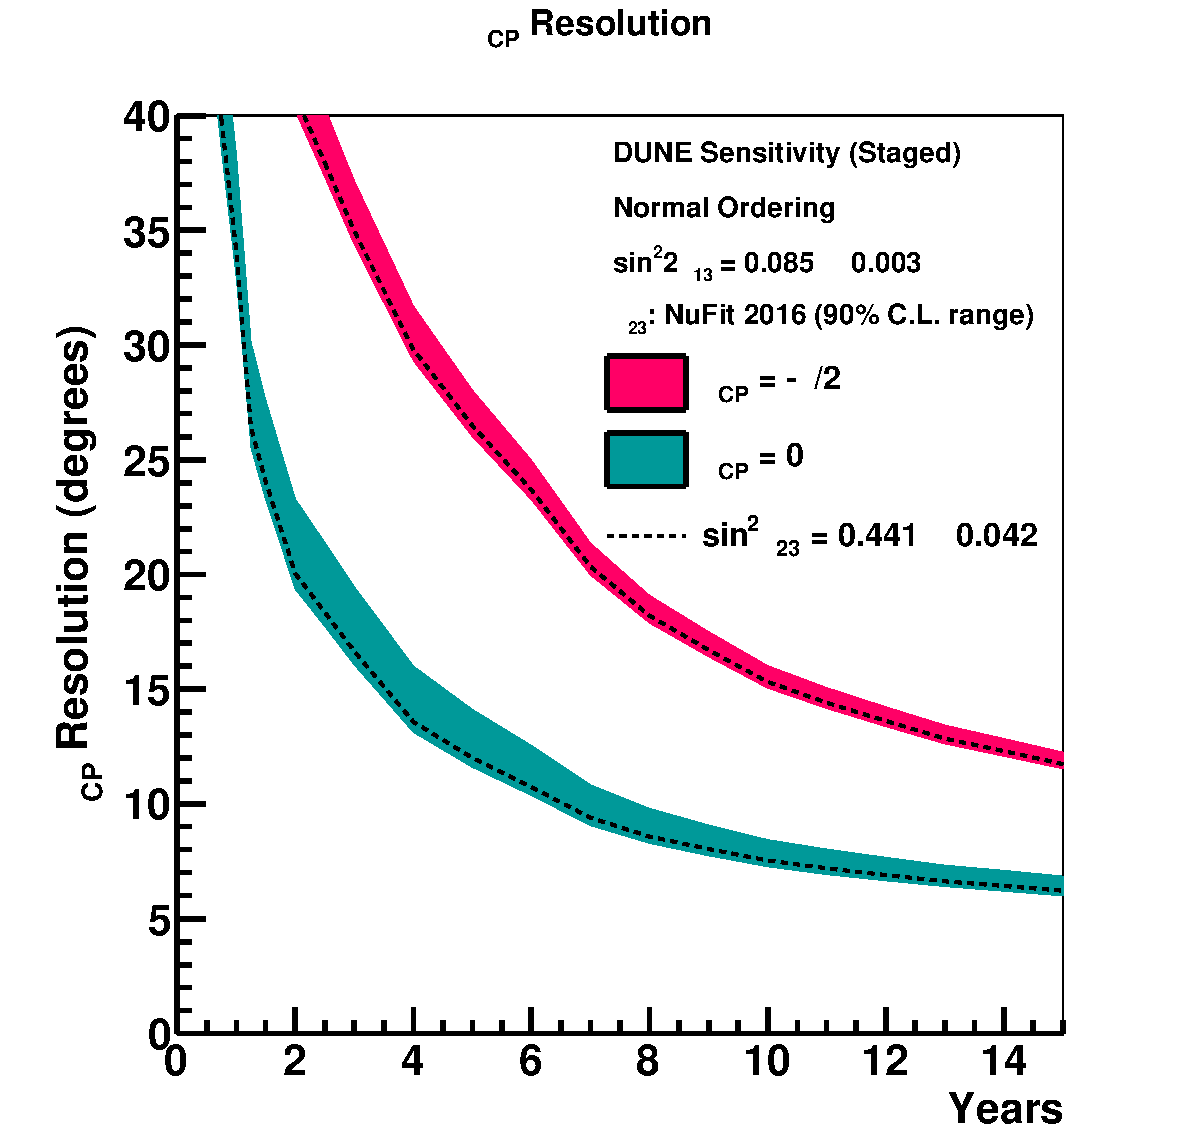
\includegraphics[width=0.5\textwidth]{resdcp_exp_staging_th23band_2017}
  \caption[The resolution with which DUNE will be able to determine the value of $\delta_{CP}$, for increasing exposures]
          {The resolution with which DUNE will be able to determine the value of $\delta_{CP}$, for increasing exposures (in years). Two bands are shown, one for a value of $\delta_{CP}$ which could cause maximal CP-violation ($\delta_{CP}$ = 90$^{\circ}$), and another where there would be no CP-violation ($\delta_{CP}$ = 0$^{\circ}$). A normal hierarchy is assumed, and the shaded region shows the range of sensitivities for the 90\% confidence level range for $\theta_{23}$ values. The dashed line shows the sensitivity for the NuFit central value of $\theta_{23}$. The figure is taken from~\citep{DUNE2377}.}
  \label{fig:DUNECPViolationRes}
\end{figure}

DUNE also aims to perform precision measurements of the neutrino mixing parameters, in order to improve sensitivity to any physics beyond the standard thee-flavour oscillation model. As discussed in Section~\ref{sec:NeutPhys}, the current best limit for the value of $\theta_{23}$ does not determine which octant it is in, specifically whether it is more than, or less than, 45$^{\circ}$. Determining the octant of $\theta_{23}$ is important, as should it be found that $\theta_{23}$ is equal to 45$^{\circ}$, it would hint at an unknown symmetry. DUNE will determine the value of $\theta_{23}$ by combining measurements of $\nu_{\mu} \rightarrow \nu_{\mu}$, and $\nu_{\mu} \rightarrow \nu_{e}$, which are sensitive to $\sin^{2}2\theta_{23}$, and $\sin^2\theta_{23}$, respectively. Figure~\ref{fig:DUNEOctantDetermination} shows the significance to which the octant of $\theta_{23}$ can be determined for different values of $\theta_{23}$. Correspondingly, Figure~\ref{fig:DUNETheta23Res} shows the resolution to which the value of $\sin^{2}\theta_{23}$ can be determined with increasing exposures. \\

\begin{figure}
  \centering
  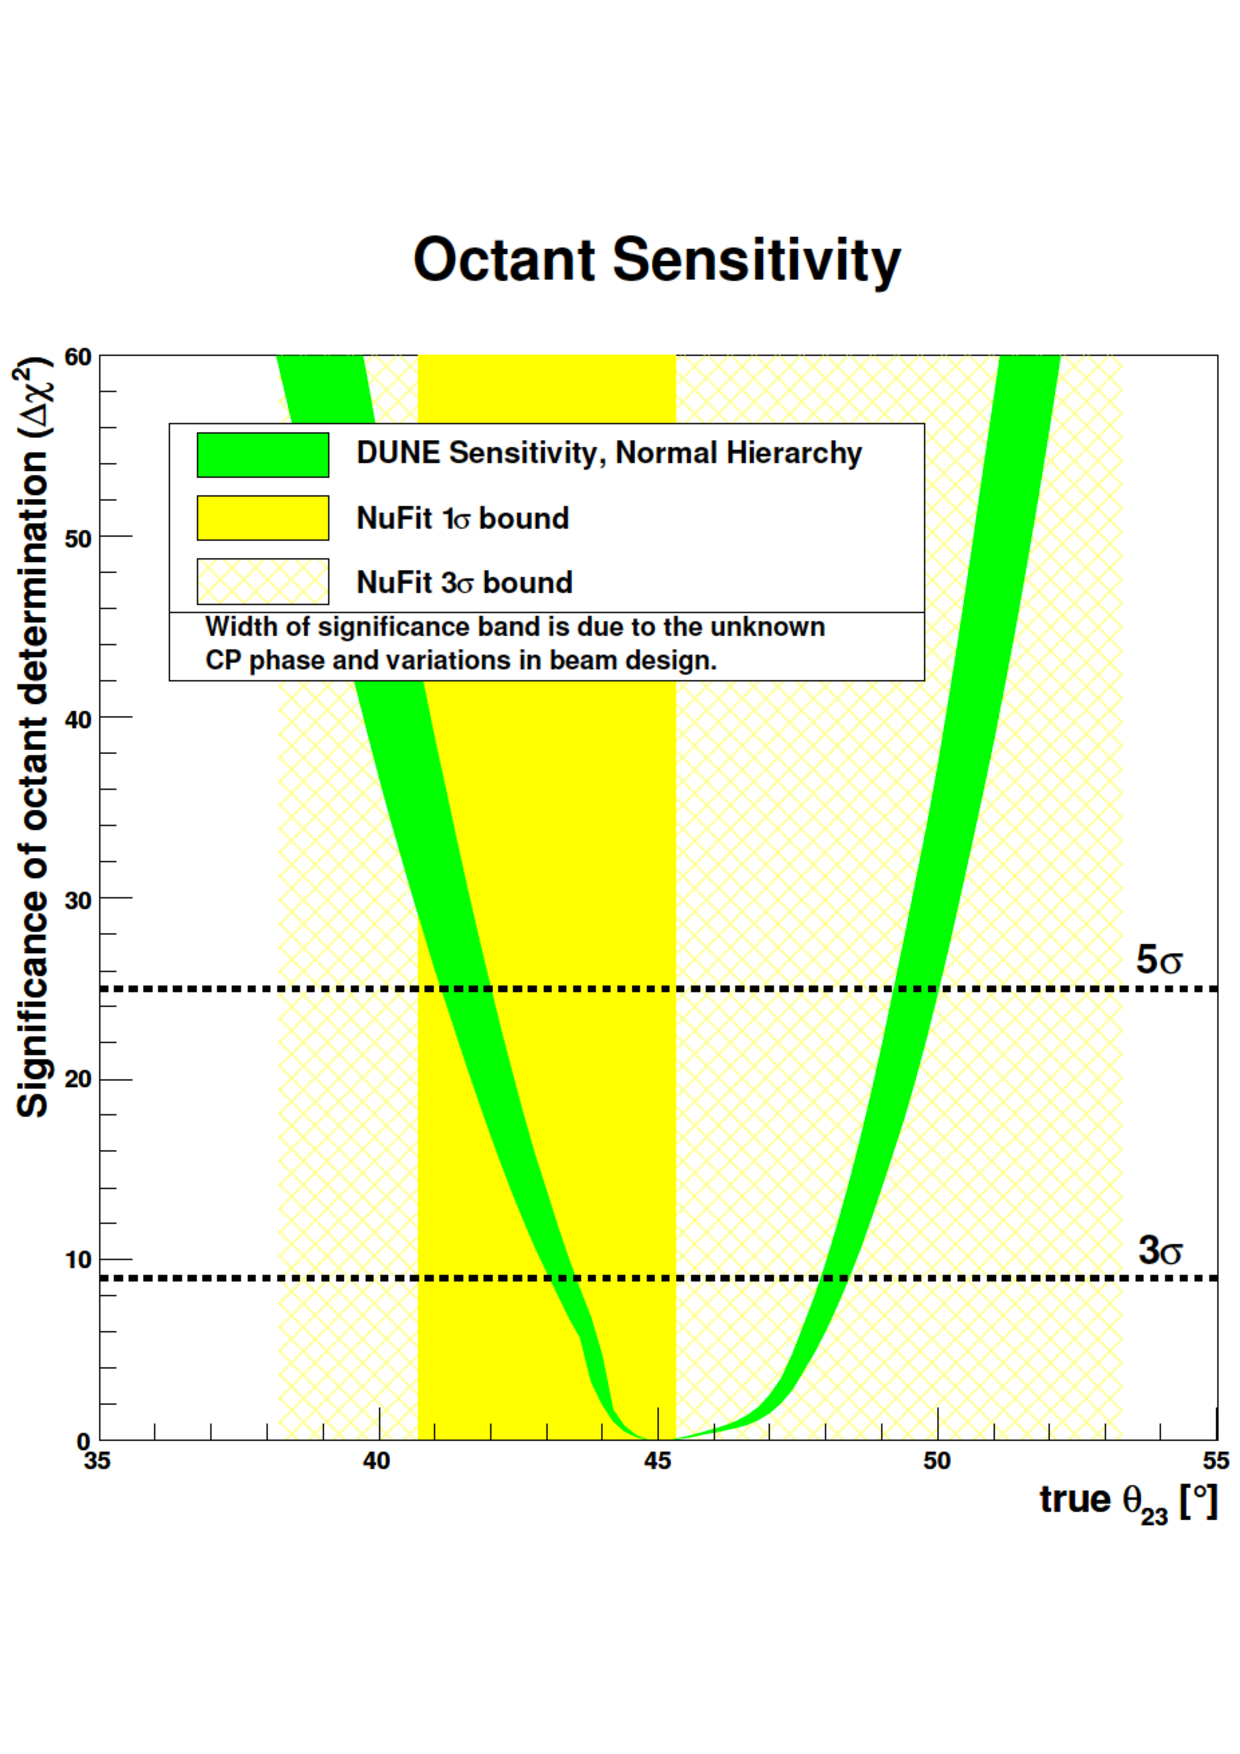
\includegraphics[width=0.5\textwidth]{DUNEOctantDetermination}
  \caption[The significance to which the octant of $\theta_{23}$ can be determined, for values of $\theta_{23}$]
          {The significance to which the octant of $\theta_{23}$ can be determined, for values of $\theta_{23}$. An exposure offering a 3$\sigma$ determination of the value of $\delta_{CP}$ for 75\% of the values of $\delta_{CP}$ is assumed. The green band shows the effect of different values of $\delta_{CP}$ and beam configurations. The yellow region show the 1$\sigma$ and 3$\sigma$ at the time of writing. The figure is taken from~\citep{DUNECDR_V2}.}
  \label{fig:DUNEOctantDetermination}
\end{figure}

\begin{figure}
  \centering
  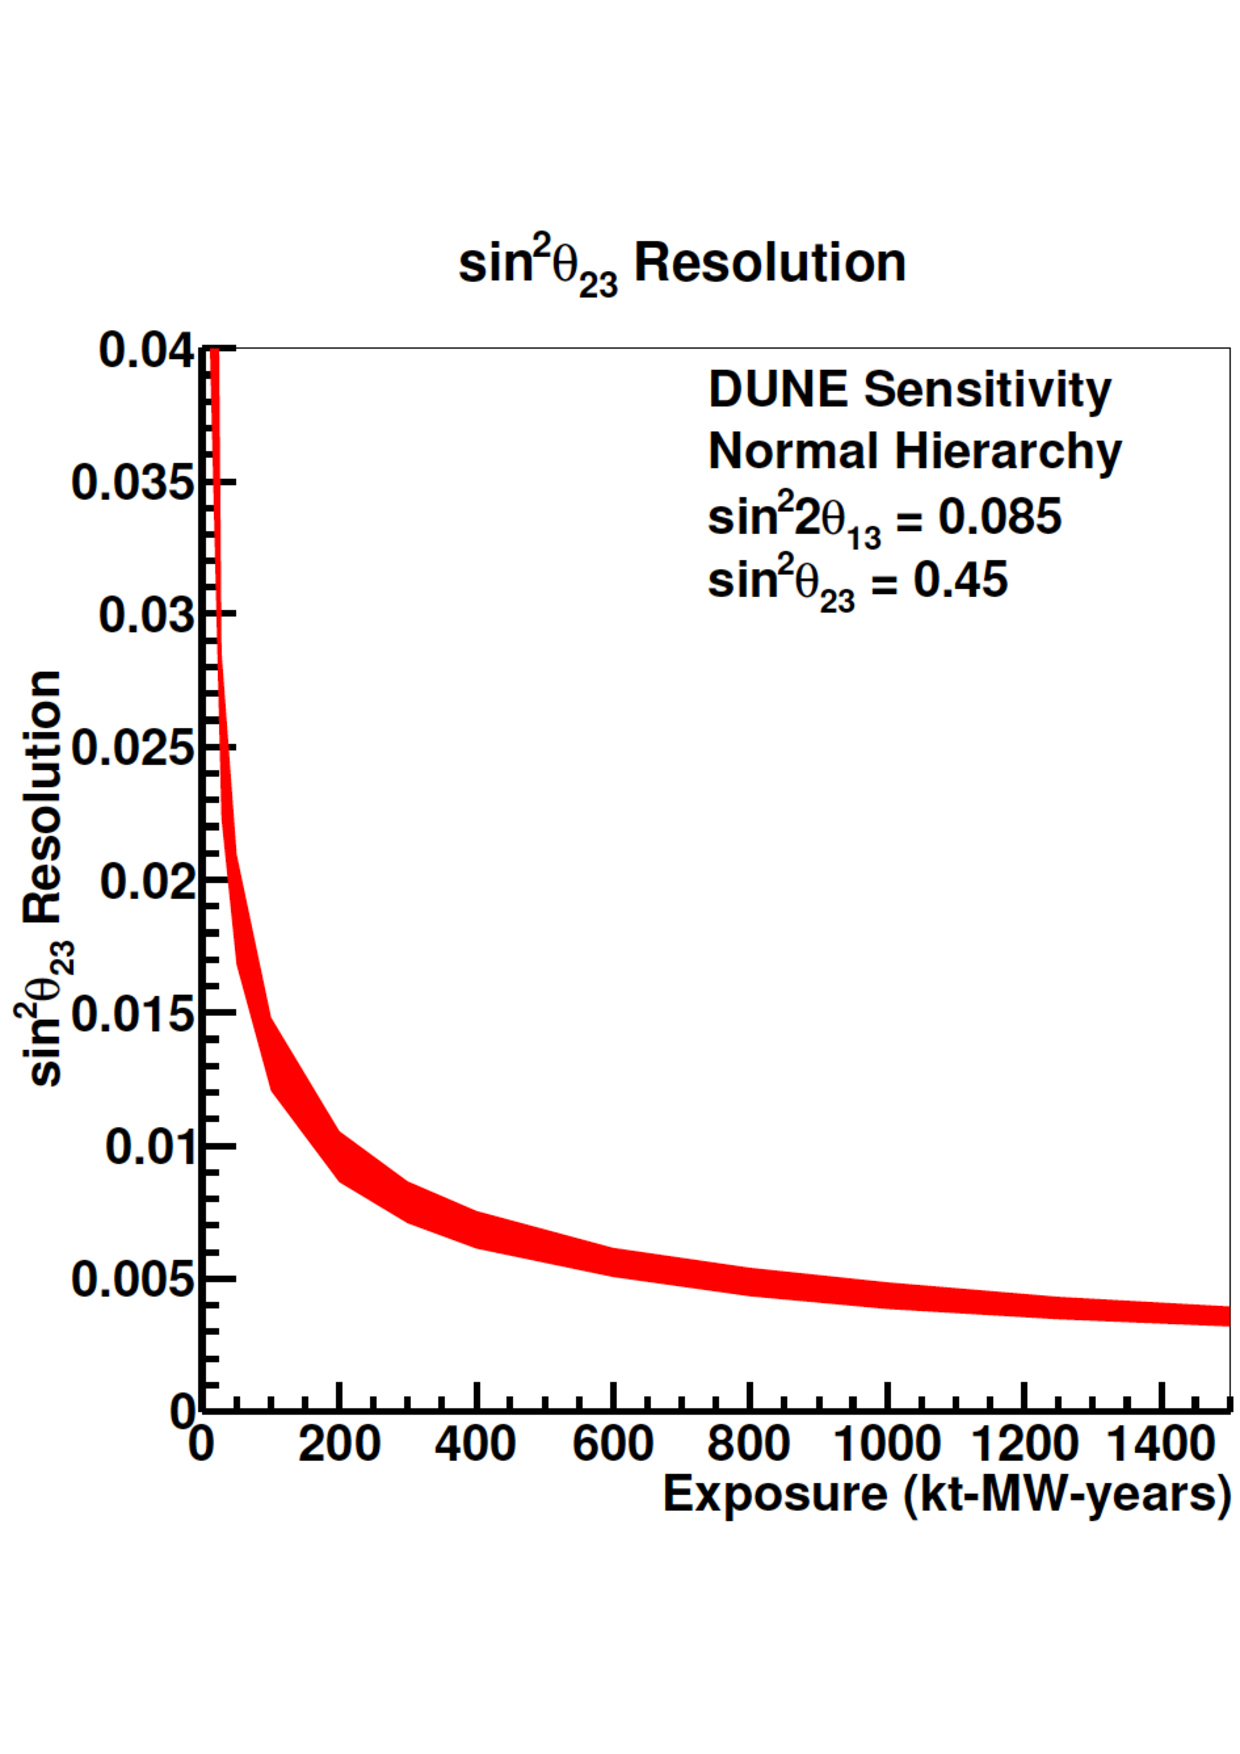
\includegraphics[width=0.5\textwidth]{DUNETheta23Res}
  \caption[The resolution with which DUNE will be able to determine the value of $\sin^{2}\theta_{23}$ for increasing exposures]
          {The resolution with which DUNE will be able to determine the value of $\sin^{2}\theta_{23}$ for increasing exposures. A normal hierarchy is assumed, and the bands show the sensitivities to the potential beam designs. The figure is taken from~\citep{DUNECDR_V2}.}
  \label{fig:DUNETheta23Res}
\end{figure}

The precision with which the values for $\sin^{2}\theta_{13}$ and $\Delta m^{2}_{31}$ can be measured by DUNE are shown in Figure~\ref{fig:DUNETheta13Res} and Figure~\ref{fig:DUNEDeltaMRes} respectively. \\ 

\begin{figure}
  \centering
  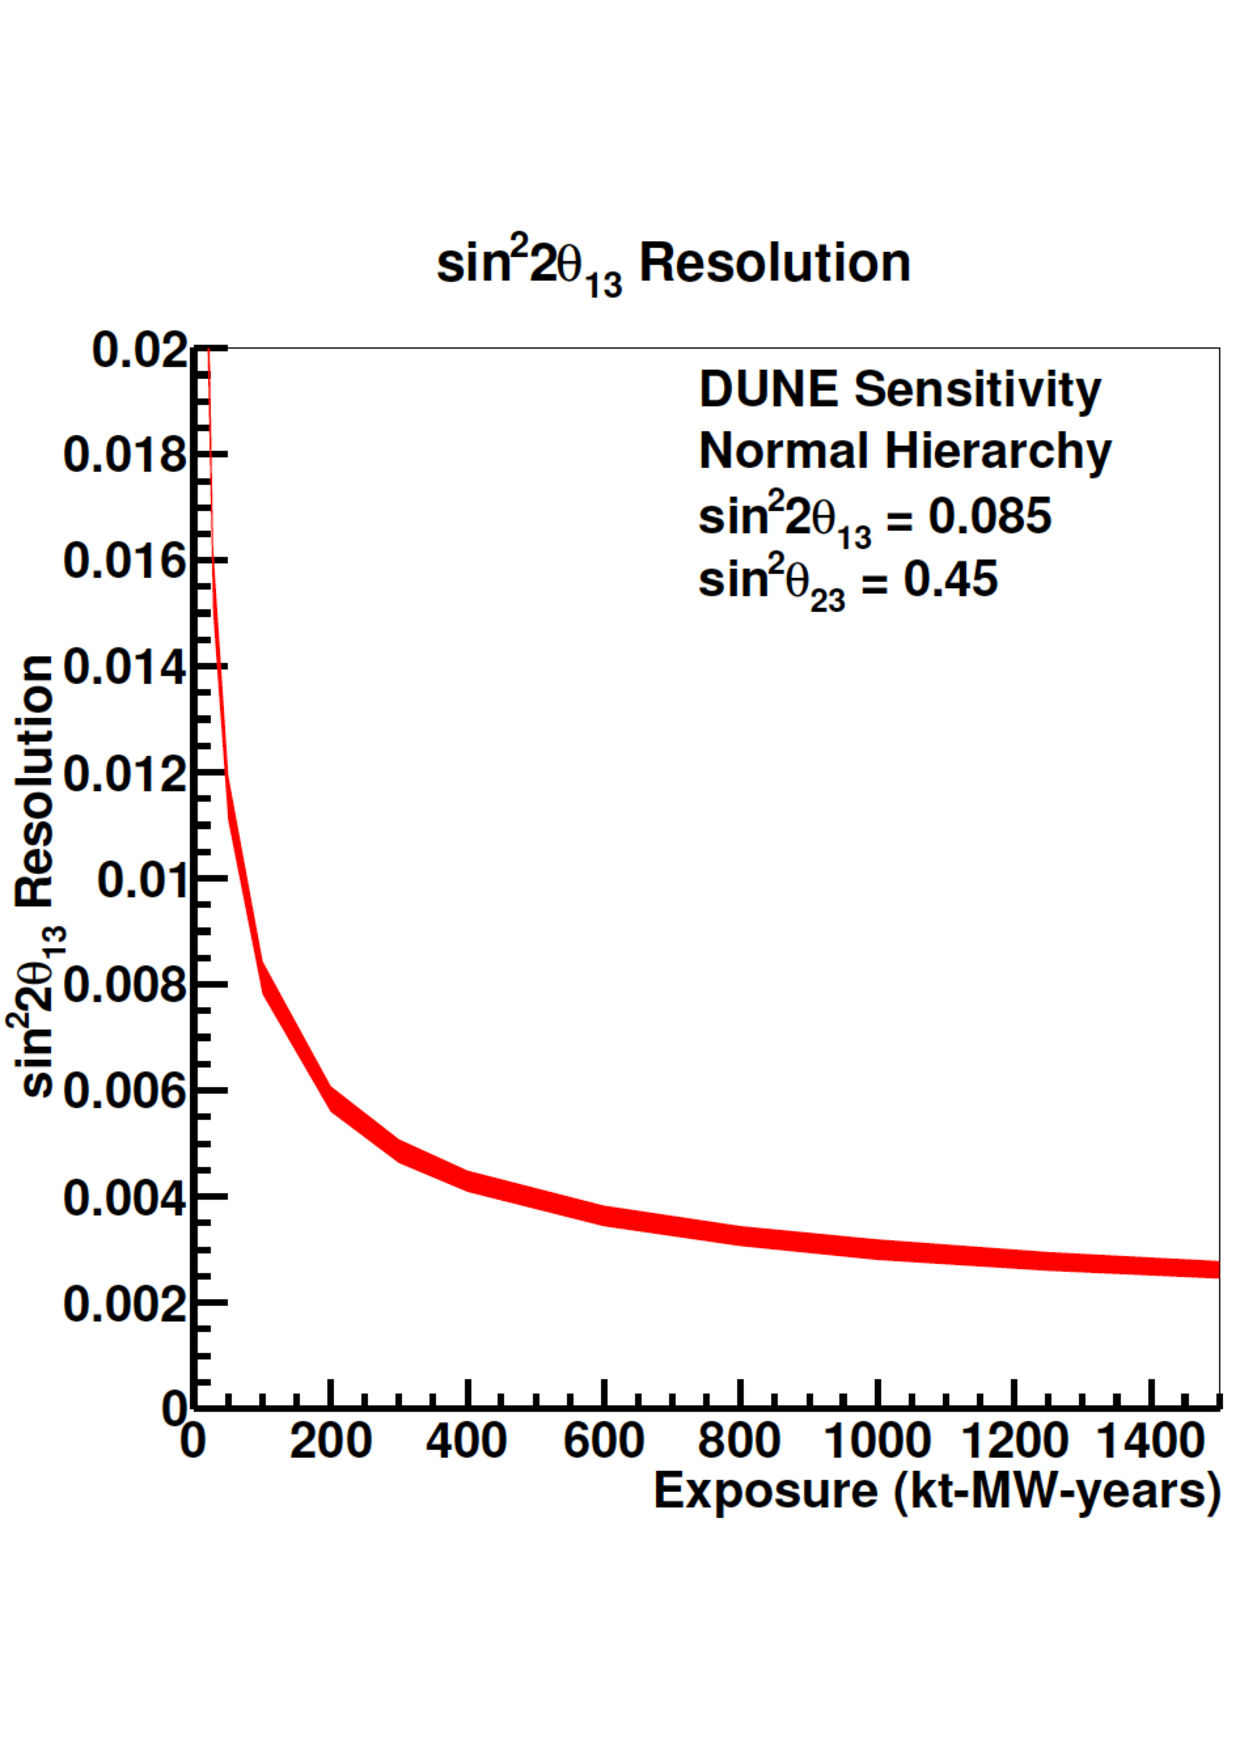
\includegraphics[width=0.5\textwidth]{DUNETheta13Res}
  \caption[The resolution with which DUNE will be able to determine the value of $\sin^{2}\theta_{13}$ for increasing exposures]
          {The resolution with which DUNE will be able to determine the value of $\sin^{2}\theta_{13}$ for increasing exposures. A normal hierarchy is assumed, and the bands show the sensitivities to the potential beam designs. The figure is taken from~\citep{DUNECDR_V2}.}
  \label{fig:DUNETheta13Res}
\end{figure}

\begin{figure}
  \centering
  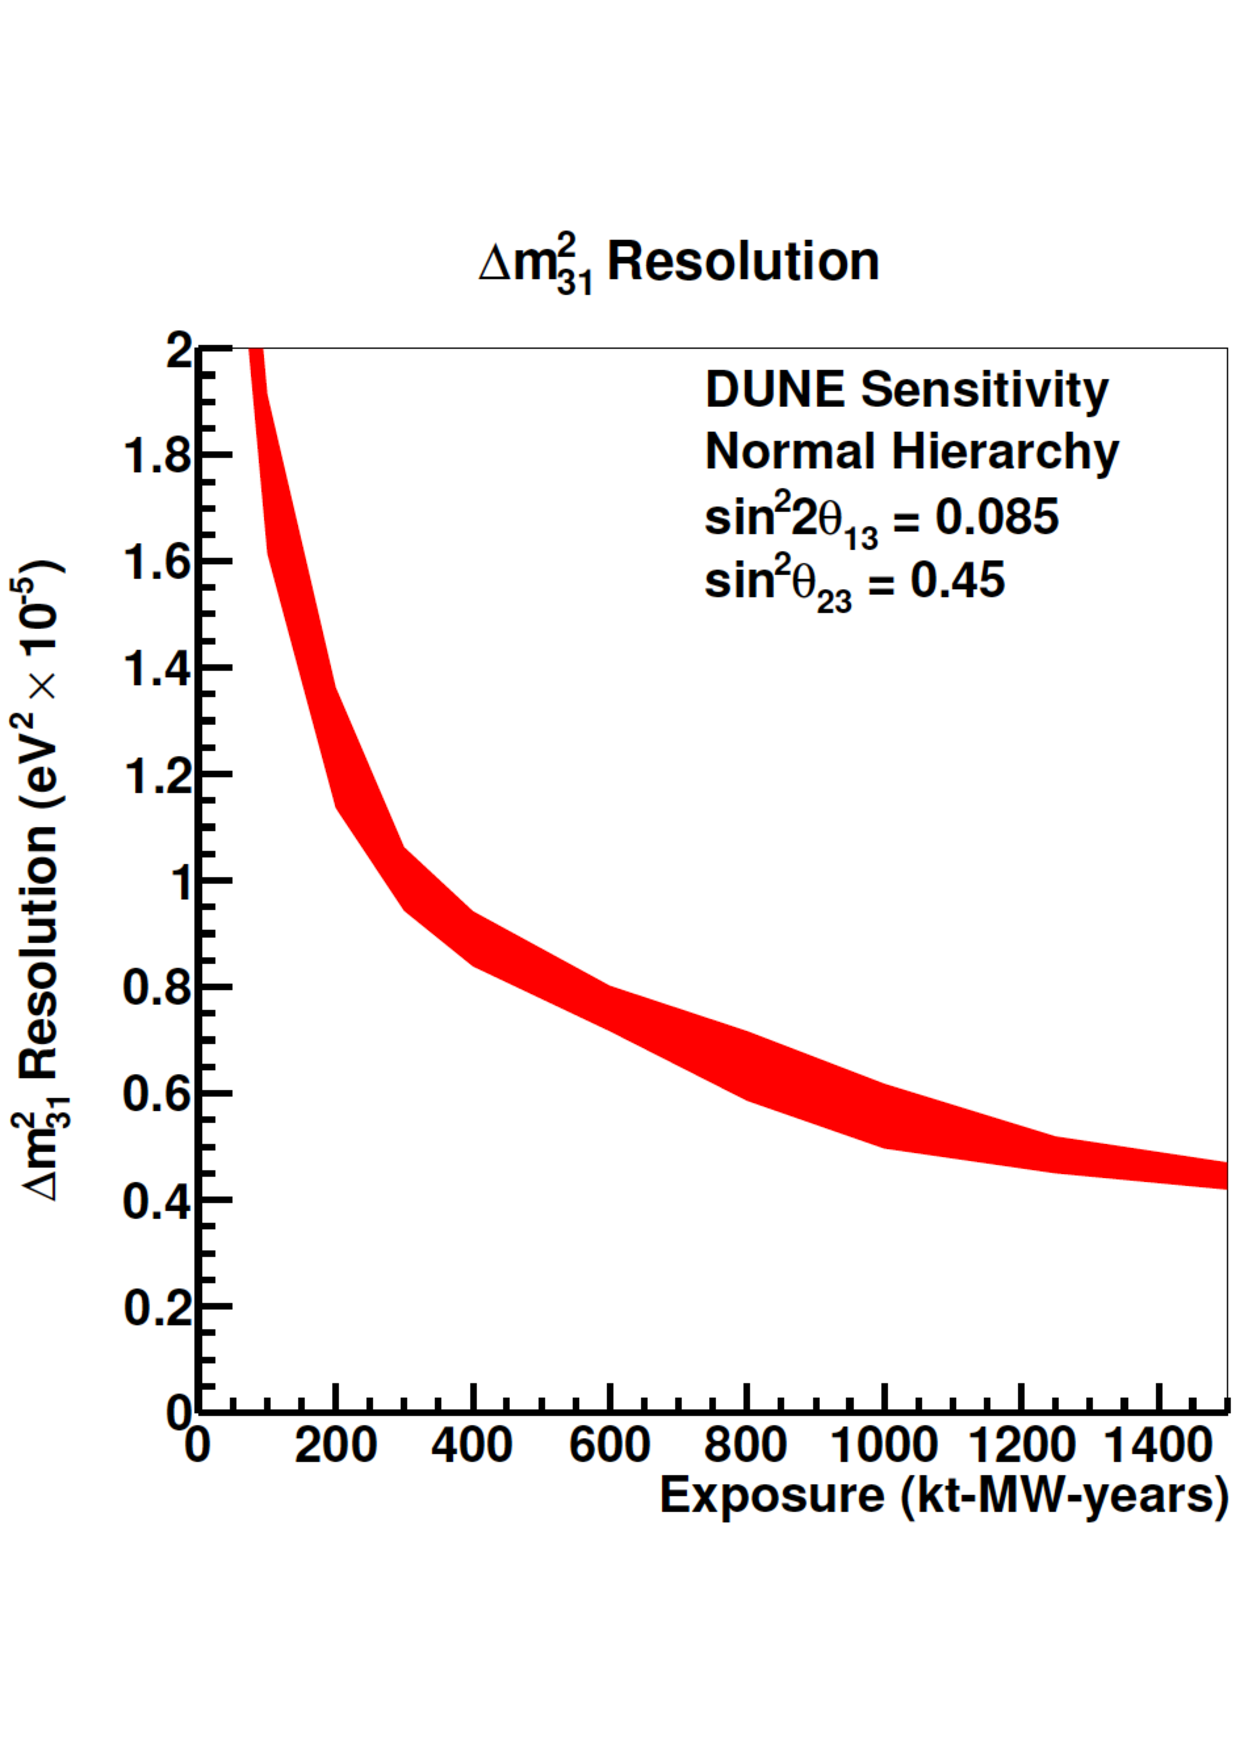
\includegraphics[width=0.5\textwidth]{DUNEDeltaMRes}
  \caption[The resolution with which DUNE will be able to determine the value of $\Delta m^{2}_{31}$ for increasing exposures]
          {The resolution with which DUNE will be able to determine the value of $\Delta m^{2}_{31}$ for increasing exposures. A normal hierarchy is assumed, and the bands show the sensitivities to the potential beam designs. The figure is taken from~\citep{DUNECDR_V2}.}
  \label{fig:DUNEDeltaMRes}
\end{figure}

The resolution to which DUNE can measure the value of $\sin^{2}\theta_{13}$ is unlikely to surpass that of reactor experiments, outlined in Section~\ref{sec:Theory_Exp}. However, DUNE will measure $\sin^{2}\theta_{13}$ using $\nu_e$ and $\overline{\nu_e}$ appearance, as opposed to $\overline{\nu_e}$ disappearance, as is done in reactor experiments. This complementary measurement of $\sin^{2}\theta_{13}$ will provide an independent constraint on the three-flavour mixing matrix. DUNE will also be able to greatly improve the resolution to which the $\Delta m^{2}_{31}$ mass splitting can be determined. \\

It is also possible to measure many of the properties of neutrino mixing using atmospheric neutrinos. This is because, as mentioned in Section~\ref{sec:Theory_Exp}, atmospheric neutrinos contain all flavors of neutrinos and antineutrinos, and cover a wide range of $L/E$ values. Also, atmospheric neutrinos are always available. This is particularly useful because, as discussed in Section~\ref{sec:DUNEDetector}, the DUNE schedule has at least one 10 kt module becoming operational before the beam is operational. As is the case in experiments such as Super-Kamiokande, DUNE can observe the differences in upwards and downwards going neutrinos. The enhanced detector resolution of DUNE, allows the possibility that features expected in neutrino and antineutrino events can be resolved. This enhanced detector resolution also allows DUNE to have a comparable sensitivity to the mass hierarchy as the proposed Hyper-Kamiokande experiment, despite having a much smaller fiducial mass~\citep{DUNECDR_V2}.  

%********************************** % 3.2 Section  *************************************
\subsection{Nucleon decay} \label{sec:DUNE_NDK}%Section - X.2.2
As presented in Section~\ref{sec:Theory_GUT}, many so called Grand Unified Theories (GUTs) predict some form of nucleon decay. Though nucleon decay has never been observed, there are still regions of phase space where nucleon decay could occur. As DUNE will be located deep underground, it will have a low background rate. This, combined with the high detector resolution of a LArTPC, means that DUNE offers an ideal candidate to continue the search for nucleon decay. \\

The search for nucleon decay in DUNE is primarily focused on two proton decay modes, $p \rightarrow e^{+} \pi^{0}$ and $p \rightarrow K^{+} \overline{\nu_{e}}$. In the first of these decay modes, the total mass of the proton should be converted into the electromagnetic showers produced by the two particles, and their net momentum should be zero. This is a signal which can be clearly identified in water Cherenkov detectors, such as Super-Kamiokande, and so is the main decay mode which these detectors look for. This decay mode should also produce a clear signal in a LArTPC such as DUNE. However, the second decay mode is particularly interesting in DUNE, as kaons should be able to be accurately identified in a LArTPC. This is not the case in a water Cherenkov detector, as the kaons produced are not energetic enough to produce Cherenkov light. Though particular emphasis will be given to the $p \rightarrow K^{+} \overline{\nu_{e}}$ decay mode in this section, the same strengths in particle identification are true for all decay modes which feature a kaon in the final state. It is also important to note that DUNE will search for all type of nucleon decays, including bound neutron decays and neutron to antineutron oscillations, the former will be given particular focus in Section~\ref{sec:DUNENDK}. \\

It is hoped that DUNE will be able to reach sensitivities to nucleon decay lifetimes of between $10^{33}-10^{35}$ years. A comparison of current, and potential lifetime limits, from a range of experiments is shown in Figure~\ref{fig:DUNE_NDK_Lifetime}. It can be seen that DUNE will provide very stringent limits to nucleon decay lifetimes, which will compete with the proposed Hyper-Kamiokande in all decay modes other than the $p \rightarrow e^{+} \pi^{0}$ decay mode. As outlined earlier, Cherenkov detectors are able to perform relatively background free studies in this channel, and so due to the much larger mass of Hyper-Kamiokande, it is able to achieve a limit which is superior to DUNE. In the other channels however, the excellent spatial resolution of LArTPCs allow DUNE to compete with, and in many cases improve on, any limit which could be set by Hyper-Kamiokande. \\

\begin{figure}
  \centering
  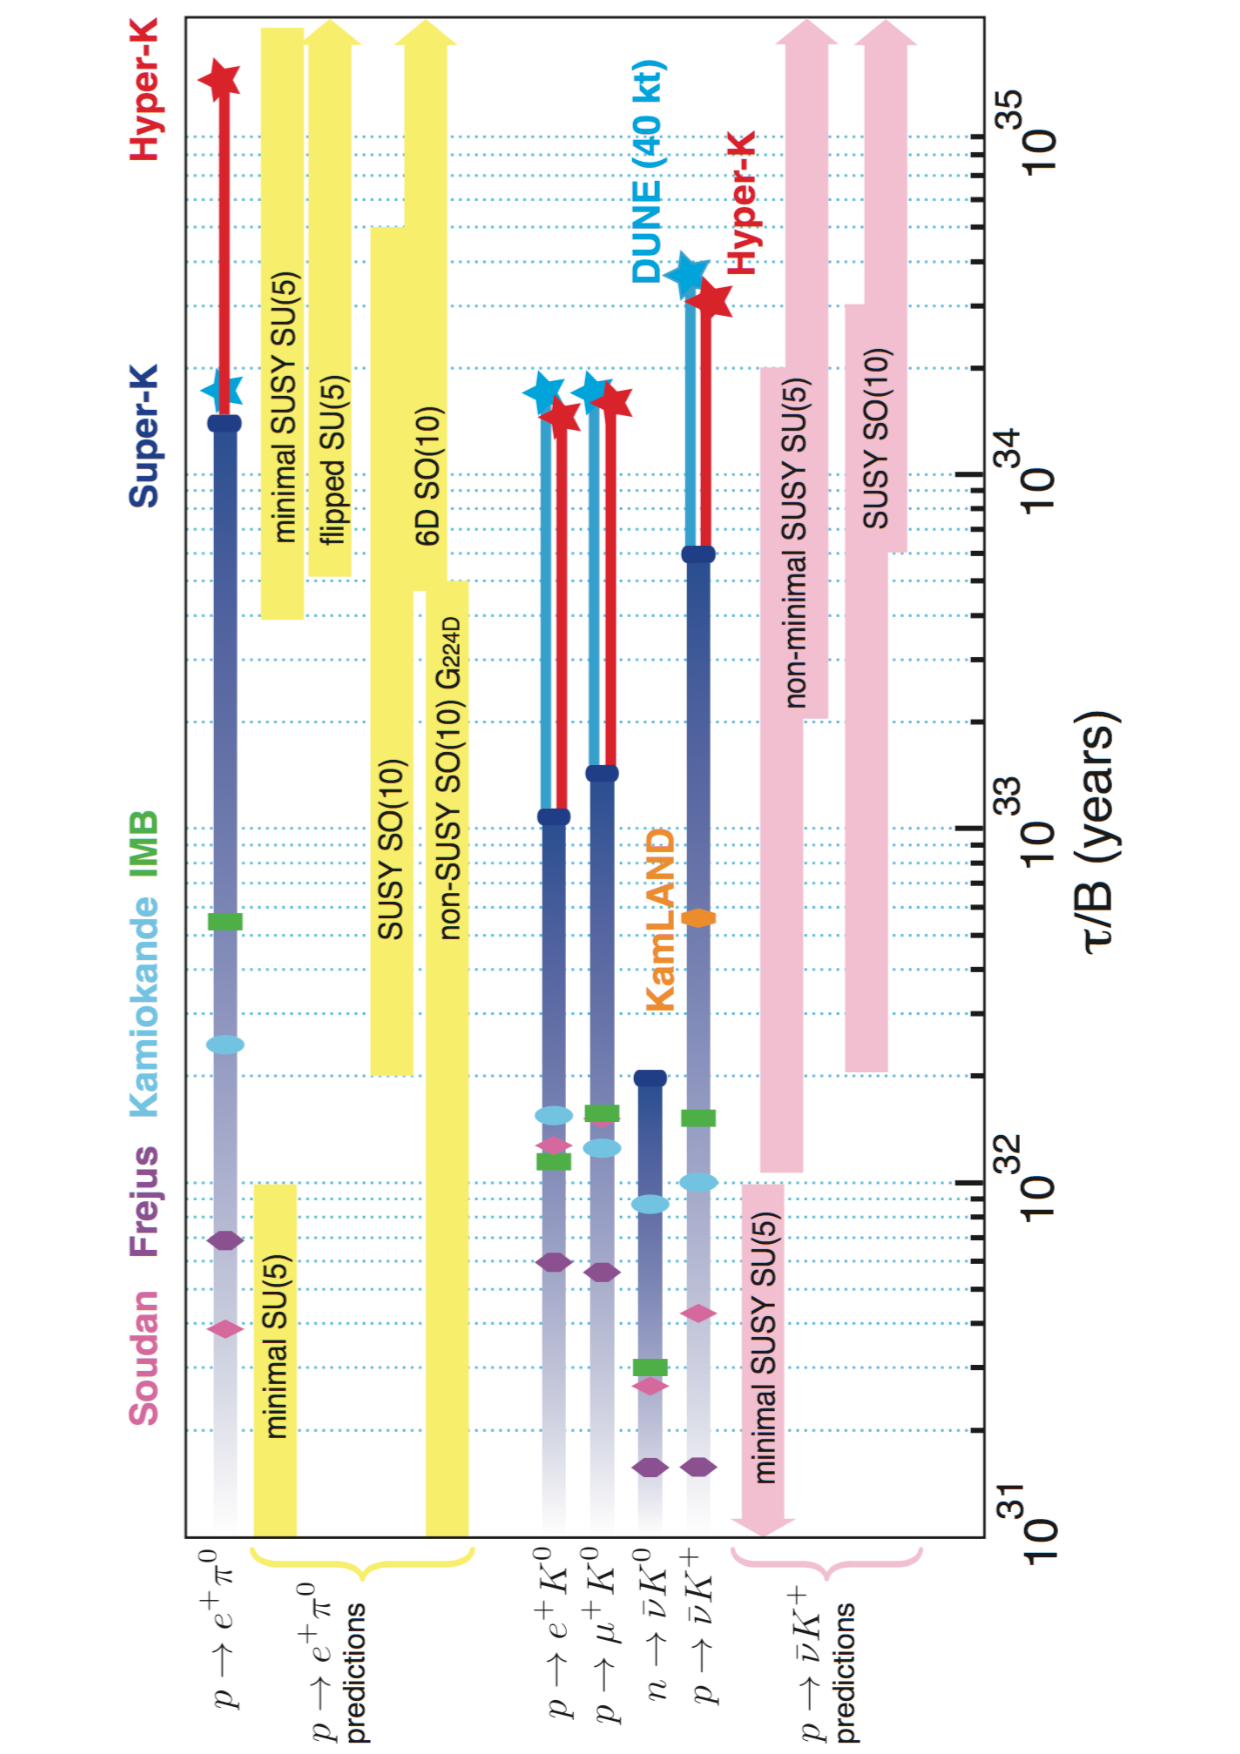
\includegraphics[width=0.8\textwidth]{NucleonDecayLimits}
  \caption[A comparison of current, and future, nucleon decay lifetime limits, compared with the ranges predicted by Grand Unifying Theories.]
          {A comparison of current, and future, nucleon decay lifetime limits, compared with the ranges predicted by Grand Unifying Theories. Coloured bars are shown for published limits by a number of experiments~\citep{PDG2012, Nishino:2012bnw}. Stars are shown for projected limits by future experiments, these limits are calculated using Poisson statistics, and include predicted background rates. The lifetimes predicted by different models are shown for the $p \rightarrow e^{+} \pi^{0}$, and $p \rightarrow K^{+} \overline{\nu_{e}}$, decay modes. The figure is taken from~\citep{DUNECDR_V2}.}
  \label{fig:DUNE_NDK_Lifetime}
\end{figure}

When calculating the expected sensitivity of DUNE to a range of nucleon decay modes, previous studies can be used~\citep{Bueno,Klinger:2015kva}. Some of the channels where one would expect a LArTPC, such as DUNE, to have an advantage in signal efficiency when compared to a water Cherenkov detector, such as Super/Hyper-Kamiokande, are shown in Table~\ref{tab:NDKLim}. The accurate tracking of the kaon, and its subsequent decay products, is the reason for the increased efficiency that is expected in LArTPCs. The ability for LArTPCs to perform tracking to this accuracy was seen by the ICARUS collaboration, using the T600 detector~\citep{PMTrack}. Figure~\ref{fig:ICARUSKaon}, shows an example event where a kaon enters the detector and is seen to decay to a muon, which subsequently decays to an electron. \\

\begin{table}
  \caption[Nucleon decay limits in DUNE and Super-Kamiokande, in some favoured decay channels]
          {Nucleon decay limits in DUNE and Super-Kamiokande, in some favoured decay channels. The current lifetime limits currently measured (Curr. limit), the estimated DUNE reconstruction efficiencies (DUNE $\epsilon$), and the estimated DUNE lifetime limit in 2034 (DUNE limit) are shown. For comparison, the published Super-Kamiokande reconstruction efficiencies (SK $\epsilon$), and the estimated Super-Kamiokande lifetime limit in 2034 (SK limit) are also shown. All lifetimes shown, are partial lifetimes, in units of 10$^{33}$ years. The table is taken from~\citep{MauryLifetime}, which uses~\citep{PDGReview}.}
  \centering
  \label{tab:NDKLim}
  %\scriptsize
  \begin{tabular}{l c c c c c}
    \toprule
    {Decay mode}                               & {Curr. limit} & {DUNE $\epsilon$ (\%)} & {DUNE limit} & {SK $\epsilon$ (\%)} & {SK limit} \\ 
    \midrule
    $p \rightarrow e^{+} \pi^{0}$              & 16.7          & 45.3              & 21.4         & 54              & 50.8       \\
    
    $p \rightarrow \pi^{+} \overline{\nu_{e}}$ & 0.016         & 41.9              & 19.8         & 54              & N/A        \\
    
    $p \rightarrow K^{+} \overline{\nu_{e}}$   & 0.051         & 41.8              & 29.7         & 11              & 2.1        \\
    
    $p \rightarrow \mu^{+} \pi^{0}$            & 6.6           & 44.8              & 21.1         & 54              & 50.8       \\
    
    $p \rightarrow K^{0} \mu^{+}$              & 1.6           & 46.7              & 22.0         & 100             & 22.2       \\
    
    $n \rightarrow \pi^{0} \overline{\nu_{e}}$ & 0.112         & 45.1              & 26.0         & 30              & 7.1        \\
    
    $n \rightarrow K^{+} e^{-}$                & 0.032         & 96                & 55.4         & 100             & 1.8        \\
    \bottomrule
  \end{tabular}
\end{table}

\begin{figure}
    \centering
  \begin{subfigure}{0.48\textwidth}
    \centering
    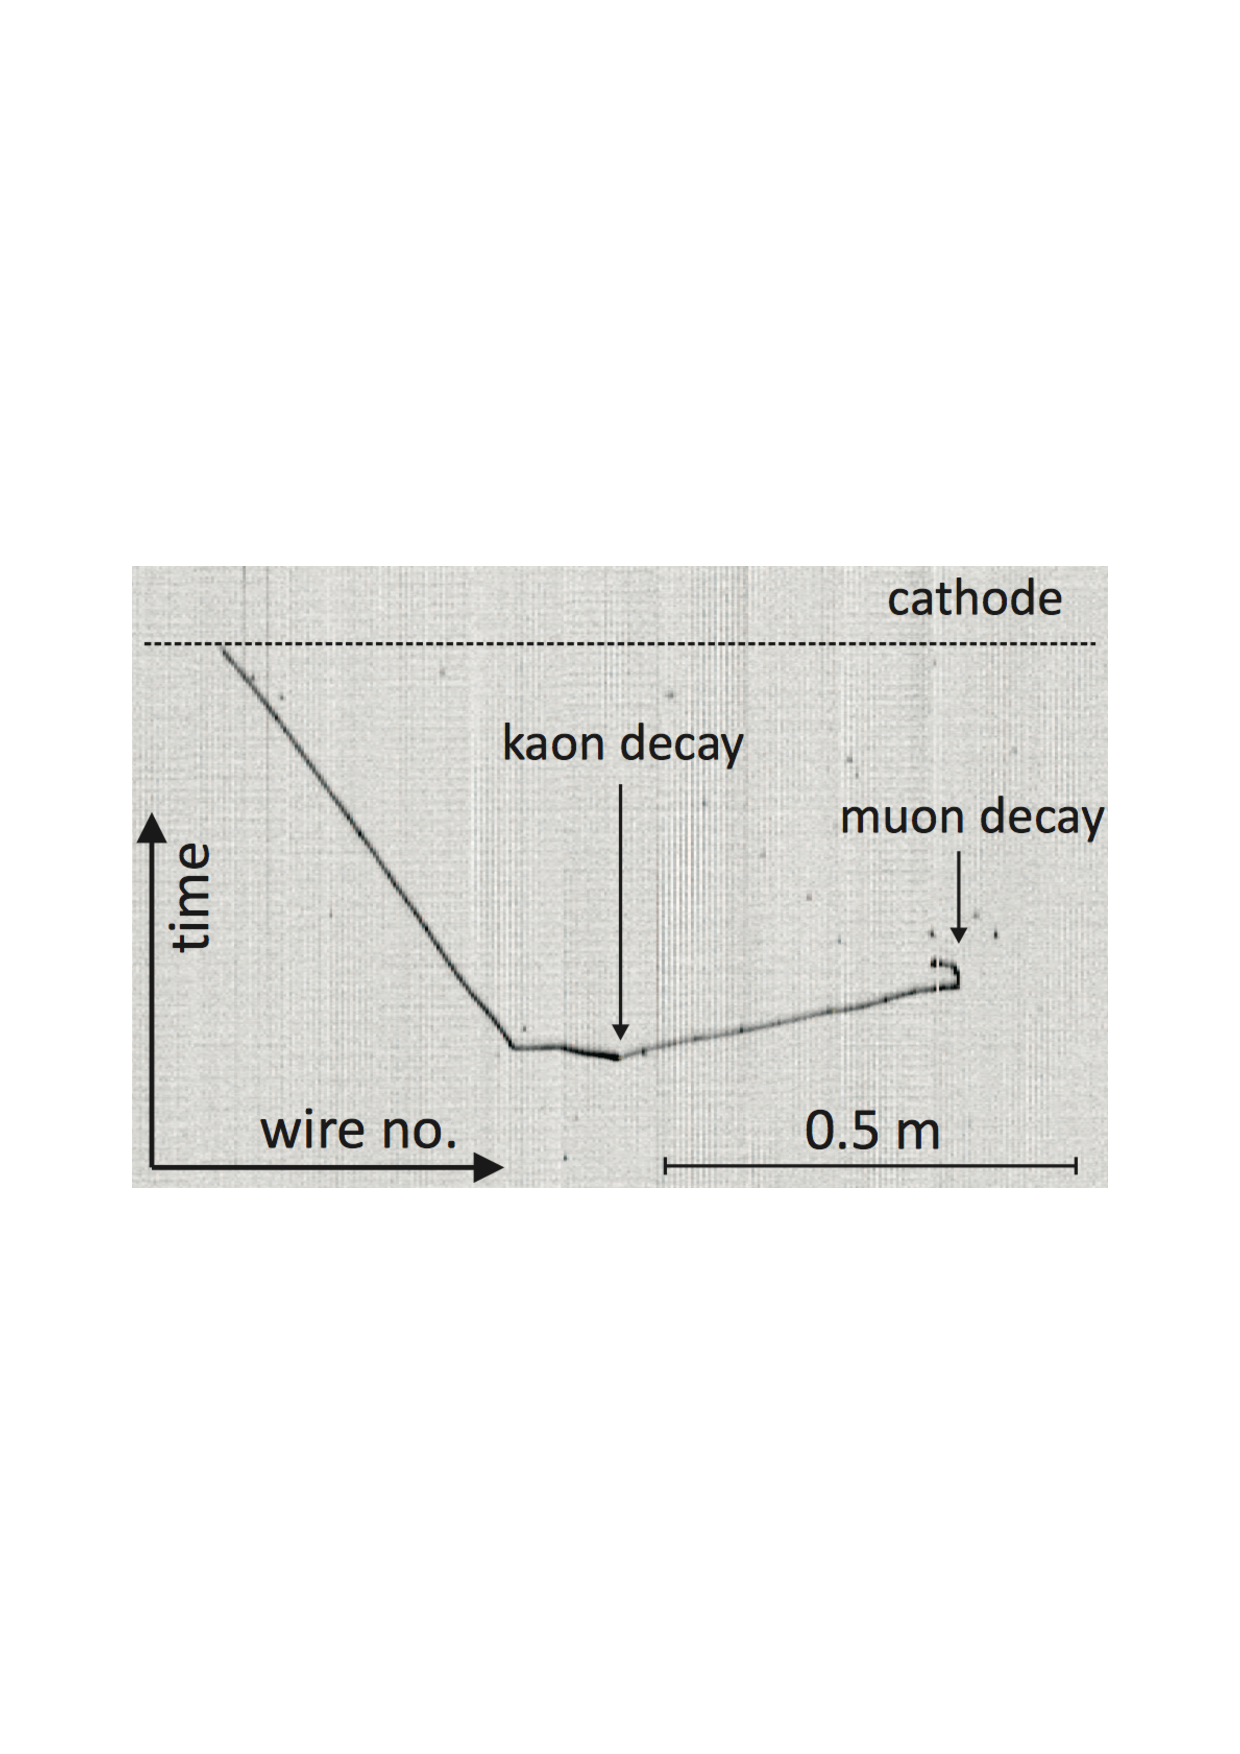
\includegraphics[width=\textwidth]{ICARUSKaon_Col}
    \caption{The collection plane view.}
  \end{subfigure}%
  \hspace{0.05\textwidth}
  \begin{subfigure}{0.42\textwidth}
    \centering
    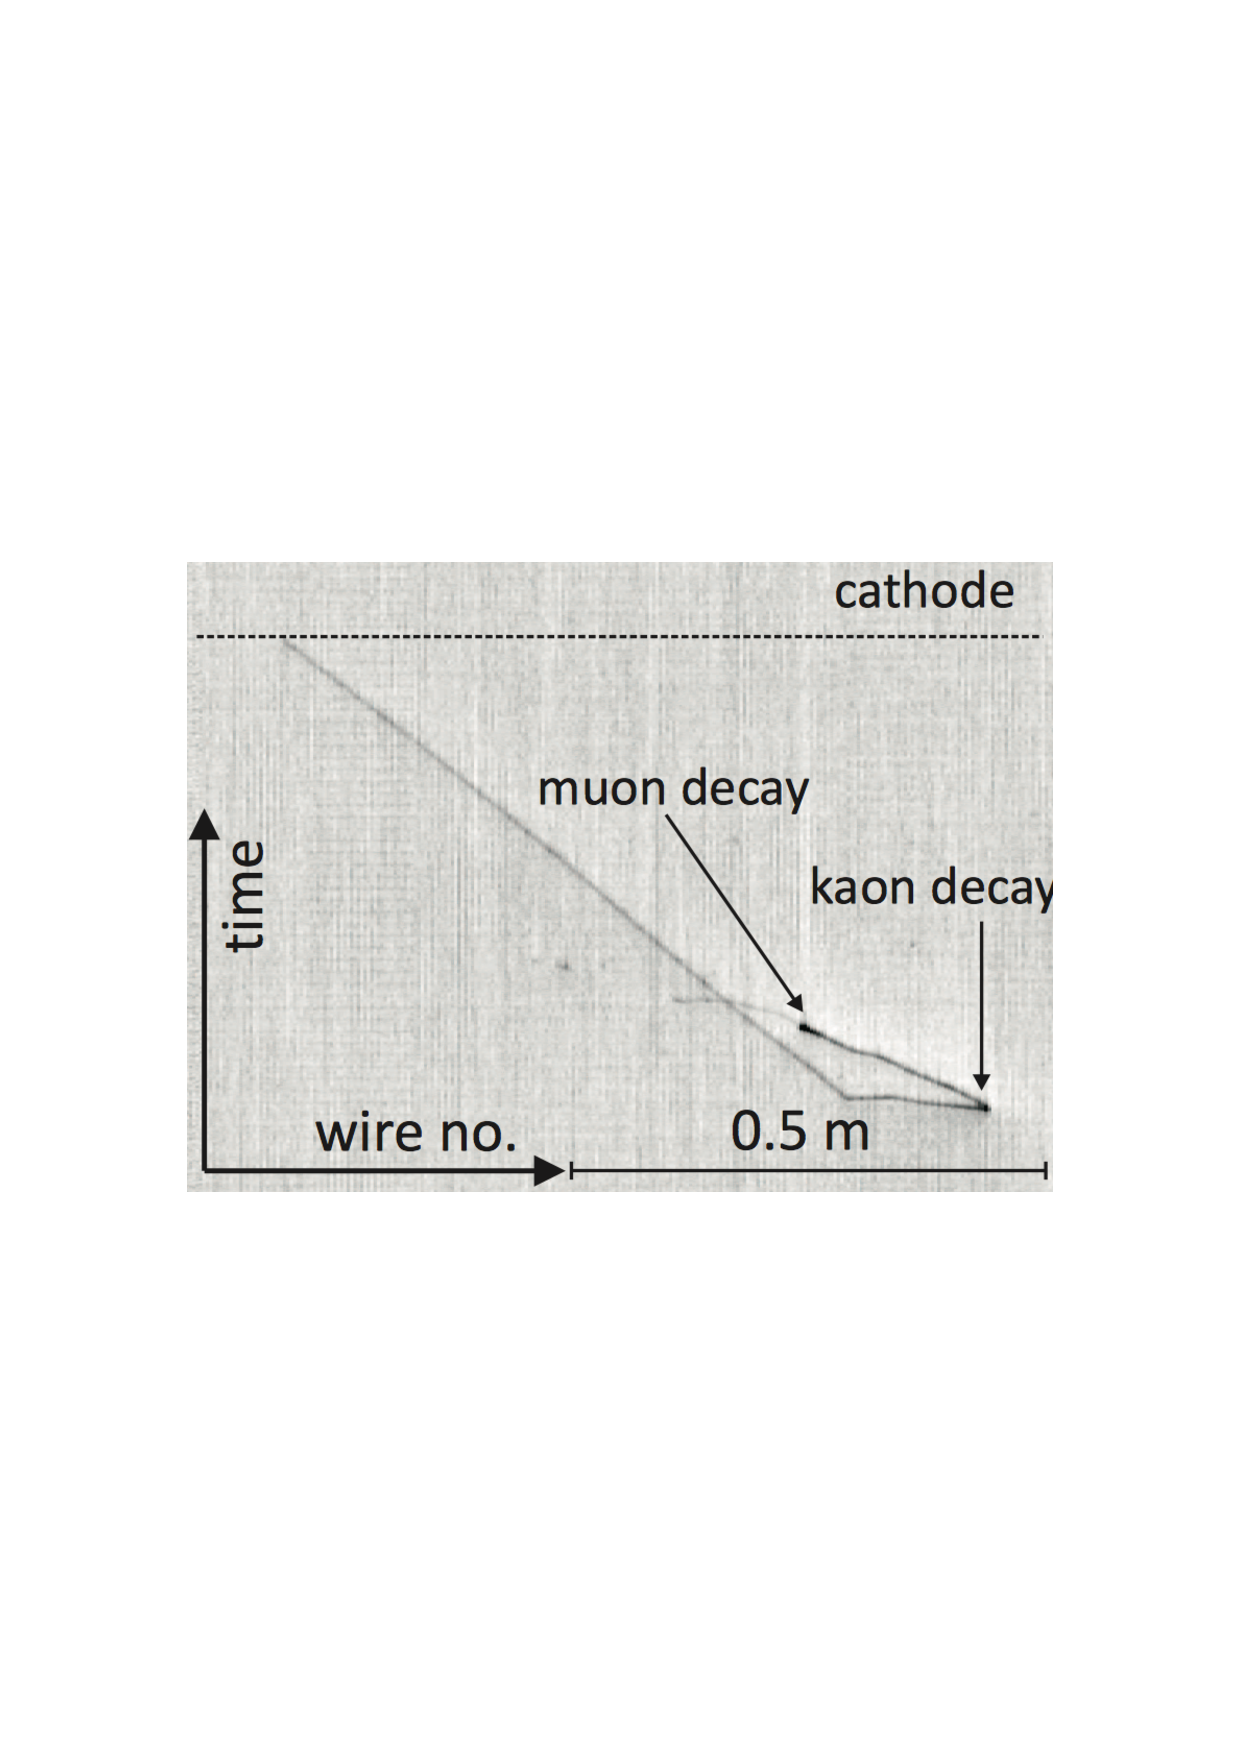
\includegraphics[width=\textwidth]{ICARUSKaon_Ind}
    \caption{The second induction plane view.}
  \end{subfigure}
  \caption[A kaon event which was observed in the ICARUS T600 detector, in the CNGS data]
          {A kaon event which was observed in the ICARUS T600 detector, in the CNGS data. Left shows the single on the collection plane, whilst right shows the signal second induction plane. The kaon enters the detector, and decays via $K \rightarrow \mu \nu$, the muon then decays via $\mu \rightarrow e \nu$. The figure is taken from~\citep{PMTrack}.}
  \label{fig:ICARUSKaon}
\end{figure}

Preliminary studies, at the time of writing the DUNE CDR documents, showed that after considering the backgrounds due to cosmic rays at depth, the backgrounds due to atmospheric neutrinos, and the impact of reconstruction failures, the number of background events for the $p \rightarrow K^{+} \overline{\nu_{e}}$ decay mode should be less than 1 per Mt yr~\citep{Klinger:2015kva, Adams:2013qkq, LBNE8836}. With a background rate this low, the observation of a single, well reconstructed event, could provide evidence of nucleon decay~\citep{DUNECDR_V2}. 

\subsection{The detection of supernova neutrino bursts and other physics opportunities} \label{sec:DUNE_Other}%Section - X.2.2
Many of the largest detectors in the World would hope to observe neutrinos from a core-collapse supernova, should one occur during their lifetimes. However, DUNE will have particularly good sensitivity to the electron flavour supernova neutrinos. This means that it should be possible to get a large, clean, supernova $\nu_e$ signal from DUNE, which is not possible using water Cherenkov detectors~\citep{KScholSND, Laha:2013hva}. The observation of neutrino interactions from a supernova would consist of short electron tracks, which were potentially accompanied by a few gamma rays. Should a core-collapse supernova occur during the lifetime of DUNE, it is hoped that many of the open questions which still remain after the observation of SN1987A~\citep{PhysRevLett.58.1494, PhysRevLett.58.1490}, could be answered by observing a large number of events. \\

The production of neutrinos from a core-collapse supernova goes as follows. Once the core of a large star reaches about 1.4 M$_{\odot}$, the core begins collapsing because the iron core begins disintegrating as electrons and protons combine. This collapse briefly stops once densities of nuclear values are reached, before the degenerate Fermi sea of electrons and electron neutrinos breaks out of the core. As this happens, the rest of the star is blasted away by a shock wave, producing the spectacular images we see of supernova remnants. This shockwave is produced as the 10$^{58}$ neutrinos, carrying 99\% of the gravitational binding energy of the core, escape the remnants of the stellar core. It takes a few seconds for all of the neutrinos to escape the stellar environment, and once they have done this, the electron neutrinos have oscillated into neutrinos and antineutrinos, of all flavours, with energies of around 10 MeV. The flavor content of the neutrinos emitted changes significantly over time, this is shown in Figure~\ref{fig:DUNE_Other_SN}. \\

\begin{figure}
  \centering
  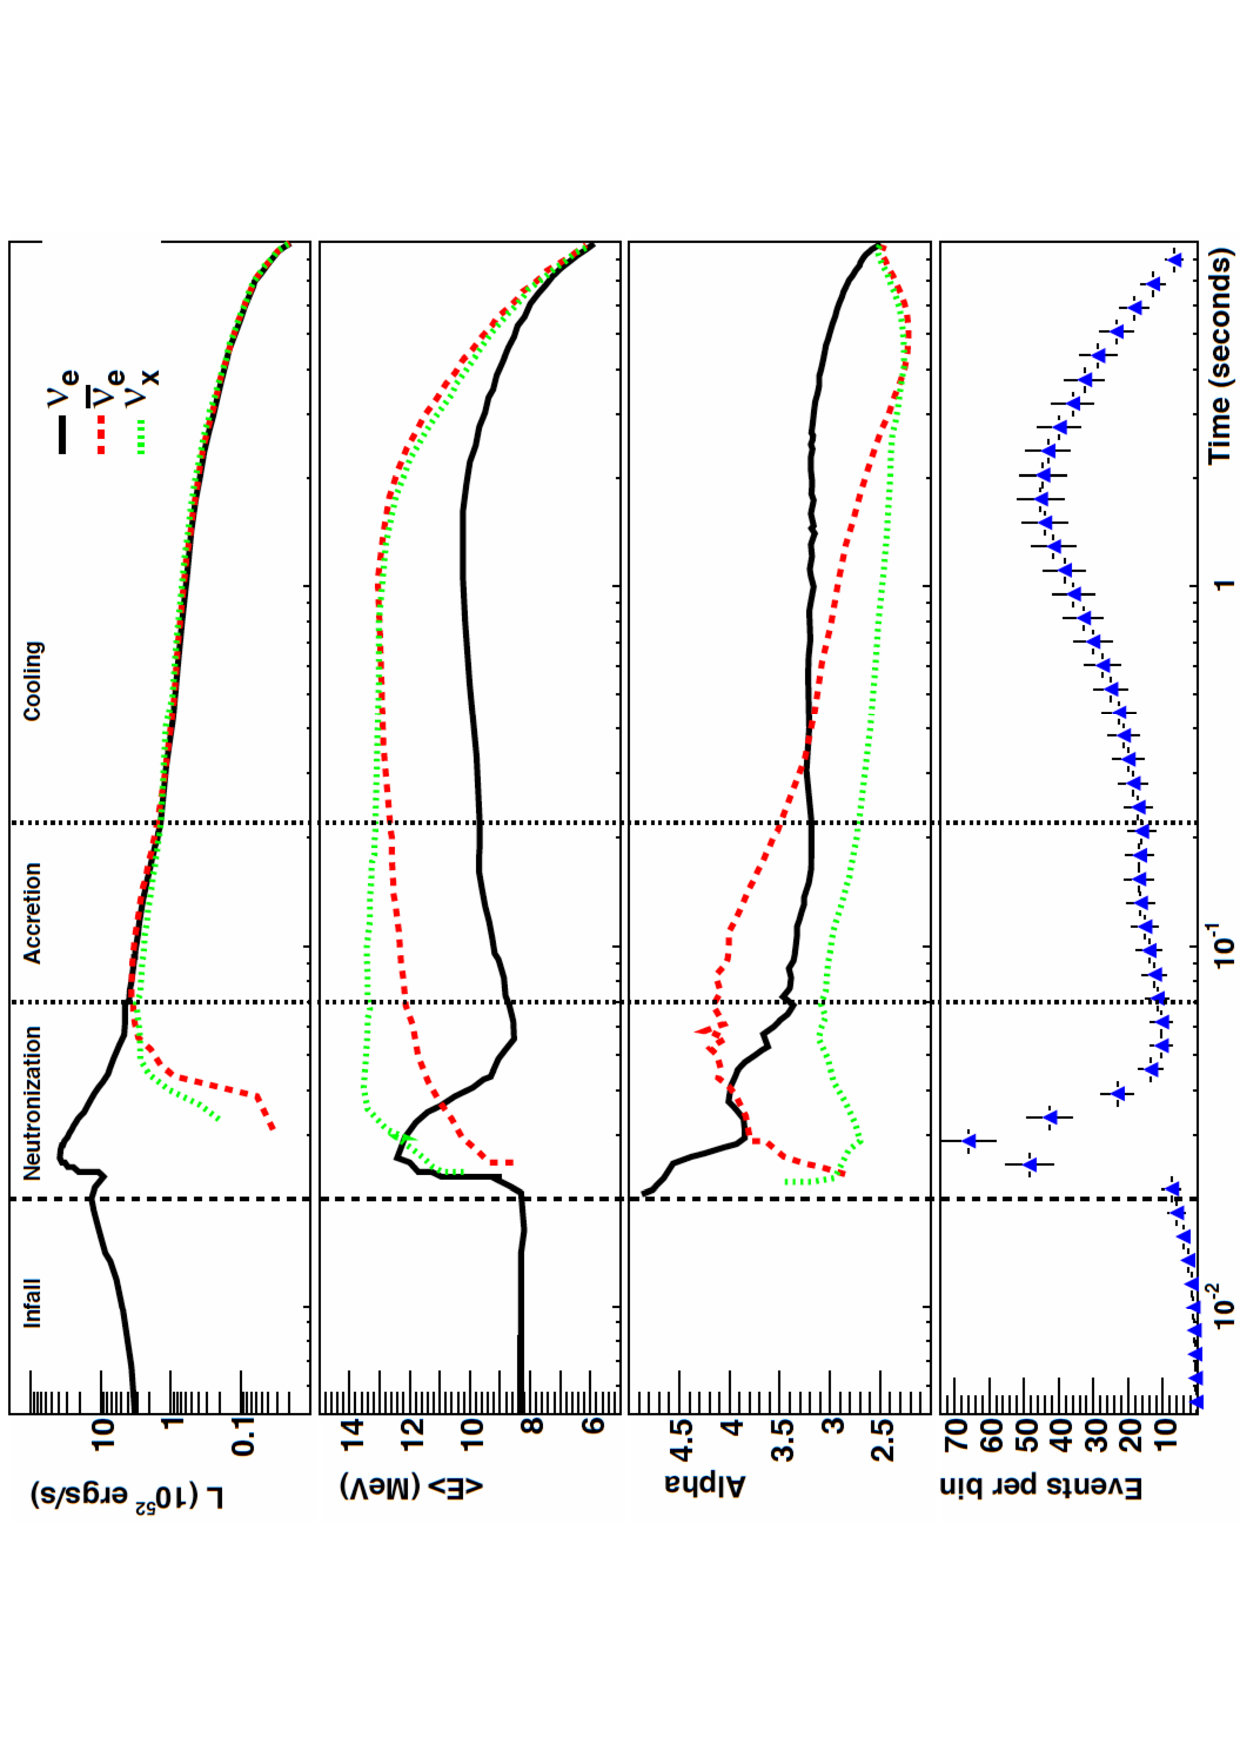
\includegraphics[width=0.8\textwidth]{SupernovaBurstProfile}
  \caption[The predicted time-dependant signal, for an electron-capture supernova, at a distance of 10 kpc from Earth]
          {The predicted time-dependant signal, for an electron-capture supernova, at a distance of 10 kpc from Earth~\citep{Huedepohl:2009wh}. It is assumed that there are no oscillations after the neutrinos are emitted. Some of the eras which are predicted in the supernova evolution are shown, and are separated by vertical dashed lines. The fluxes of $\nu_e$, $\overline{\nu_e}$, and $\nu_x$ are shown. From top to bottom, the luminosity, the neutrino energy, the `pinching' parameter, and the total number of observed events are shown, as a function of time. The figure is taken from~\citep{DUNECDR_V2}.} 
  \label{fig:DUNE_Other_SN}
\end{figure}

The model used in Figure~\ref{fig:DUNE_Other_SN} is just one of many, but most models predict that in the full DUNE 40 kt detector, around 3000 events should be observed for a supernova at a distance of 10 kpc. This reduces to the observation of a few events for a supernova in the Andromeda galaxy, which is around 780 kpc away. The observation of a supernova within the Milky Way would allow a large suite of topics to be analysed. These include, but are by no means limited to: measurements of the neutrino mass splittings, measurements of the neutrino mixing parameters, measurements of neutrino ``self-refraction'' (possible due to the high density of neutrinos around the supernova), tests of Lorentz and CPT invariance, and of course testing all aspects of the predictions made my models of supernova~\citep{DUNECDR_V2}. \\

There are also other physics aspects which DUNE could make progress in. One such aspect is the indirect searches for WIMPs. This is possible because, should a flux of high energy neutrinos be observed, which originate from regions of high mass, such as the Sun, it could support the idea of dark matter annihilation. Searches for these interactions have been performed by IceCube~\citep{Aartsen:2012kia} and \citep{Choi:2015ara}, but have not observed any signals. It is hoped that with the increased angular resolution of LArTPCs the number of background events could be substantially reduced though~\citep{DUNECDR_V2}. Other aspects where DUNE could make contributions are in searches for the diffuse supernova neutrino background~\citep{Beacom:2010kk}, searches for neutrinos from accretion disks~\citep{Caballero:2011dw}, and searches for black-hole/neutron start mergers~\citep{Caballero:2009ww}. \\

The result of this, is that there is a very compelling case for building a LArTPC at depth, which is of the scale of 40 kt.\\

%********************************** % Fourth Section  *************************************
\section{Path to building DUNE - The 35 ton prototype} \label{sec:The35tonDetector}  %Section - X.4
One extremely important aspect of DUNE which has not yet been addressed, is the need for prototypes. The DUNE FD modules represent an increase in size by more than an order of magnitude, when compared to existing LArTPCs. It is therefore necessary for a robust prototyping schedule to be performed. A brief outline of this prototyping effort is shown in Figure~\ref{fig:DUNEProtSched}. It should be noted that experiments not associated with DUNE which also use LArTPCs, will also feed into the development of DUNE by improving the technology used in LArTPCs. For this reason MicroBooNE and SBND are shown in Figure~\ref{fig:DUNEProtSched}, but experiments not shown in Figure~\ref{fig:DUNEProtSched} such as ArgoNeut and LArIAT, will also feed into the development of DUNE through the improvements which they make to LArTPC technology. \\

\begin{figure}
  \centering
  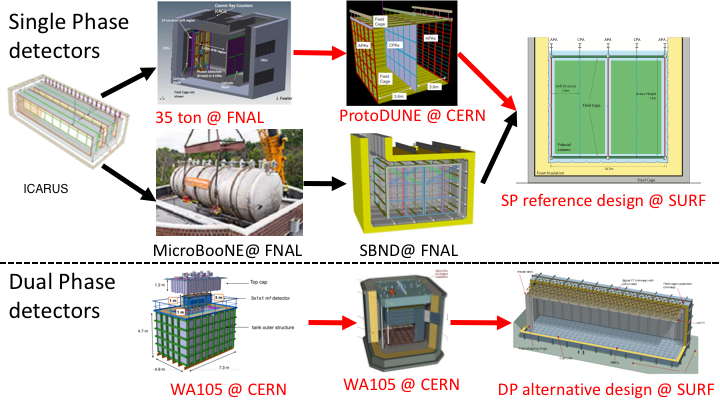
\includegraphics[width=0.98\textwidth]{PrototypeSched}
  \caption[An overview of the DUNE prototyping schedule, including complementary experiments]
          {An overview of the DUNE prototyping schedule, including complementary experiments. Top shows the experiments which utilise single phase LArTPC designs, whilst bottom shows experiments which utilise a dual phase design. The experiments which are part of the DUNE prototyping program are shown in red. The figures are taken from~\citep{MarkReviewJuly2015, DUNECDR_V4}.}
  \label{fig:DUNEProtSched}
\end{figure}

As shown by Figure~\ref{fig:DUNEProtSched}, the 35 ton is the first prototype under the umbrella of the DUNE experiment, for the single phase detector design. As such, the 35 ton provides a test bed for many of the novel aspects of the detector design required for the DUNE FDs. This testing was done during two running periods, the Phase 1 run from November 2013 - February 2014, and the Phase 2 run from November 2015 - March 2016. Chapters~\ref{chap:Cameras},~\ref{chap:35tonSim}, and~\ref{chap:35tonData}, will focus on some of the studies performed in preparation for, and during the Phase 2 run. \\ 

The primary goal of the Phase 1 run was to verify that a detector with a membrane cryostat could achieve, and maintain, the high levels of LAr purity which are required to perform the physics which DUNE hopes to achieve. It was also designed to show that it was possible to achieve this high level of purity without the need to fully evacuate the detector prior to filling, but that this could instead be achieved by performing a ``piston purge.'' This ``piston purge'' had previously been demonstrated by the Liquid Argon Purity Demonstrator (LAPD)~\citep{LAPD}, which the 35 ton was built next to, at Fermilab's PC-4 facility. The process by which the ``piston purge'' was performed is as follows. Firstly, room temperature argon is pumped into the detector, displacing the air in the detector. Once the purity is no longer seen to improve, a gas/liquid spray is used to slowly cool the detector. The injection of the spray introduces turbulence into the gas in the detector, which causes the entire cryostat to cool, meaning that there are no large temperature differences in the cryostat. Upon the completion of the cooldown, filling of the LAr commences, and LAr purification is performed using the installed recirculation loop. Using this purification method, electron lifetimes of 3 ms were observed, and maintained for many days at a time, demonstrating that membrane cryostat technology is capable of producing and maintaining high purity LAr~\citep{35tonMontanari, 35tonHahn}. \\

A detector similar to ProtoDUNE (outlined below), was originally planned to follow the Phase I run, however, funding constraints meant that this detector (at the time part of LBNE) got cancelled, and so the 35 ton was repurposed to contain a TPC. This repurposed 35 ton detector is the 35 ton Phase II run. The TPC which was installed had many of the features which are present in the single phase reference design, these include:
\begin{itemize}
\item Modular APAs with wrapped wires, collecting charge form multiple drift volumes.
\item Vertical and horizontal gaps between APAs. The Phase II run must show that it is possible to stitch particle tracks across, and through, APA frames.
\item APAs and electronics which are immersed in the LAr.
\item Waveguide-style photon detectors, installed inside the APA frames.
\item A field cage built using FR4 printed circuit board.
\item A DAQ which is capable of taking triggerless operation.
\end{itemize}
All of these features are central to the single phase DUNE detector design, and so demonstrating the successful operation of a detector with these properties is an important step in realising DUNE. Getting the Liquid Argon Software (LArSoft) framework (outlined in Section~\ref{sec:LArSoft}) ready for data taking required extensive simulation work, some of which is presented in Chapter~\ref{chap:35tonSim}. \\

In total four APAs were installed in the 35 ton cryostat, each collecting charge from two drift volumes, to give a total of 8 TPCs. As the drift volume for the 35 ton was limited to around 2.5 m, it was not possible to use TPCs with the drift length which will be present in the DUNE FD design. As such, it was decided that the TPCs would either have a ``long'' drift volume of 2.23 m, or a ``short'' drift volume of 0.27 m. These lengths were chosen so as to represent a reasonable drift distance in the ``short'' drift volume, whilst also maximising the ``long'' drift distance. The four APAs which were installed were done so, so as to have two ``long'' APAs, of roughly the length of proposed the LBNE APA frames, and two ``short'' APAs, stacked on top of each other, sandwiched between the two ``long'' APAs. This orientation allowed for both vertical, and horizontal gaps to be produced, over which reconstruction algorithms could attempt to stitch tracks. A total of 8 photon detectors were installed in the APAs, with 3 PDs in each of the ``long'' APAs, and 1 PD in each of the ``short'' APAs. A schematic of the 35 ton cryostat, with the TPC installed is shown in Figure~\ref{fig:35tonSchem}. \\

\begin{figure}
  \centering
  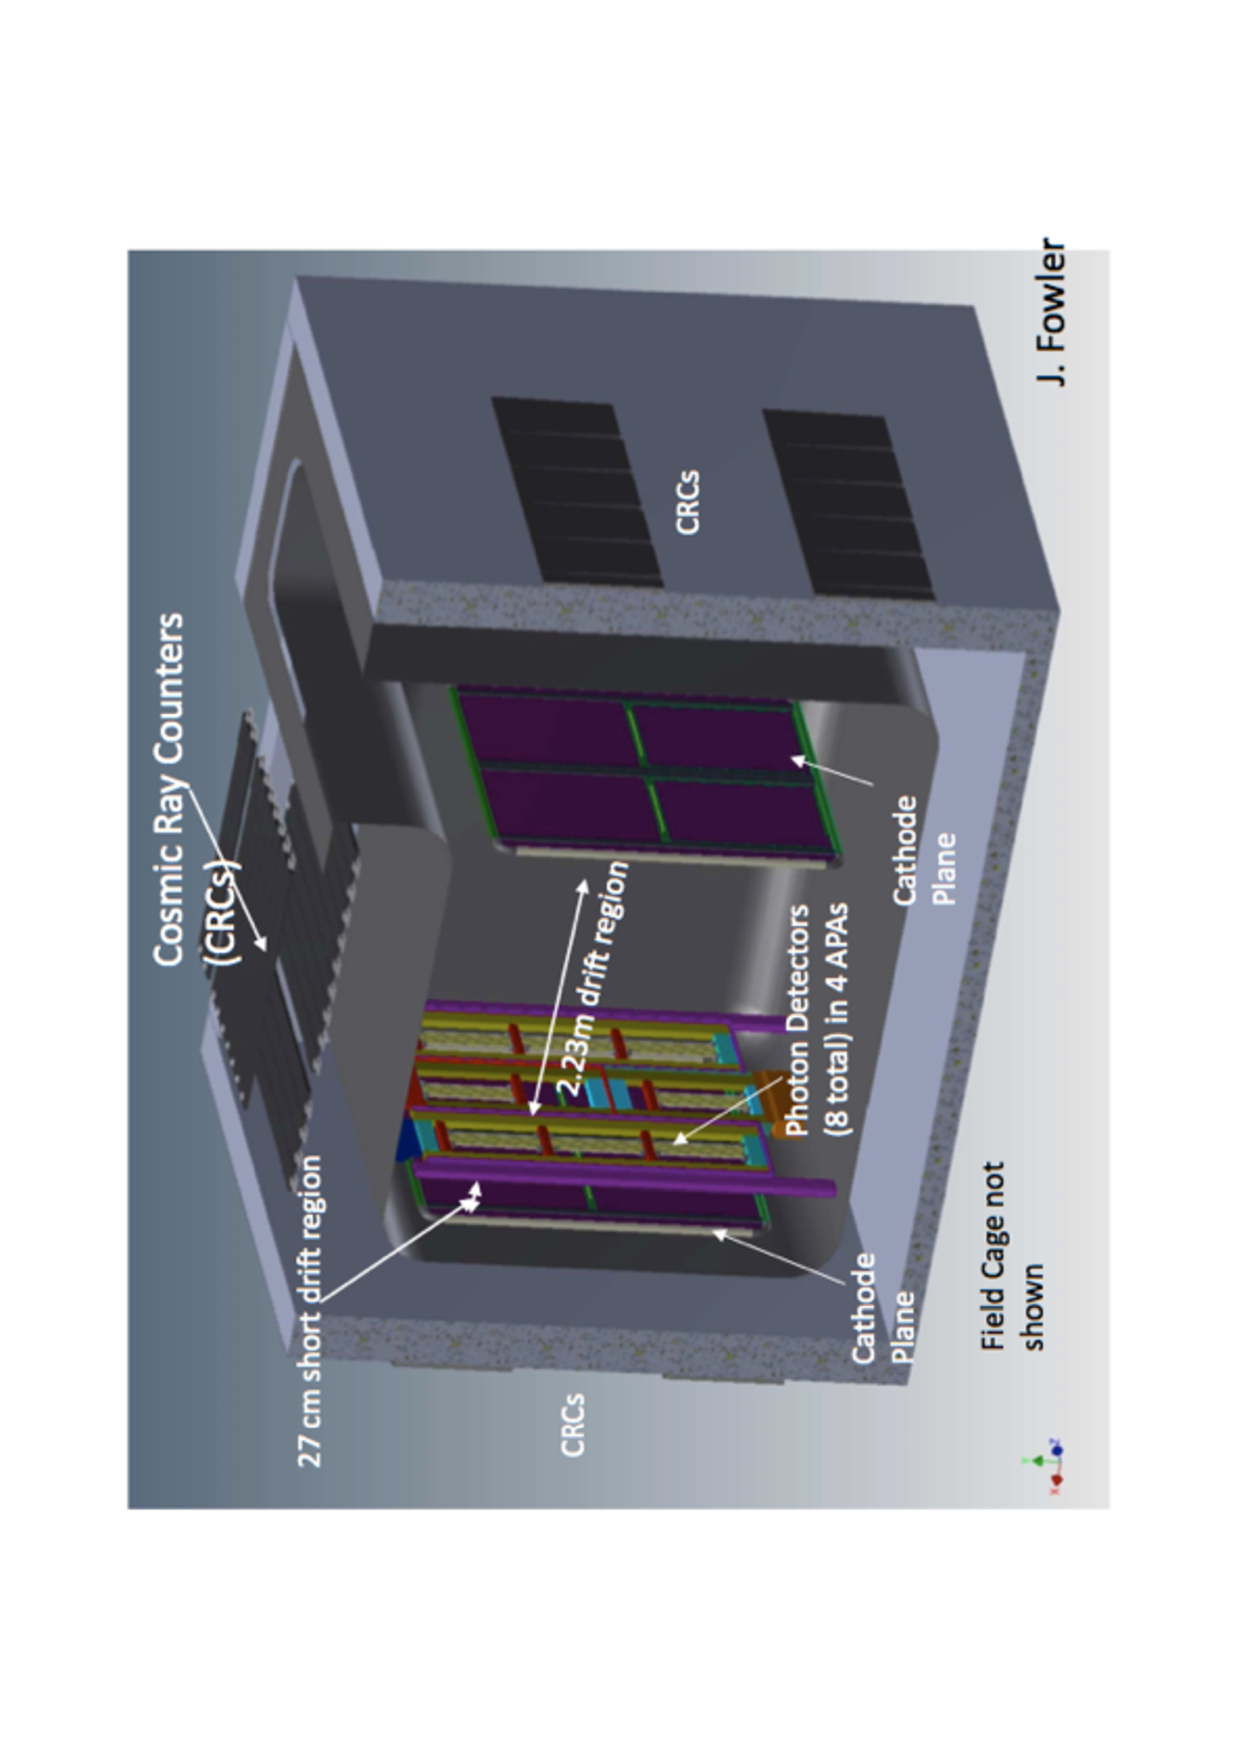
\includegraphics[width=0.85\textwidth]{35tonSchem}
  \caption[A schematic representation of the TPC installed in 35 ton prototype, for the Phase II run]
          {A schematic representation of the TPC installed in 35 ton prototype, for the Phase II run. The cathode planes (purple), photon detectors (yellow), APAs (bounded blue regions), cosmic rays counters (outer black rectangles), and the two drift volumes (2.23 m and 0.27 m) are shown. The 35 ton vessel (spotted grey), and steel contained (black) are also shown. The field cage is not shown. Cryogenic piping for the detector is placed within the cryostat, to the right of the cathode plane associated with the ``long'' drift. The figure is taken from~\citep{DUNECDR_V4}.}
  \label{fig:35tonSchem}
\end{figure}

Figure~\ref{fig:35tonSchem}, also shows a system of Cosmic Ray Counters (CRCs) on the outer edges of the cryostat walls. These were installed so as to be able to easily gather a set of cosmic muons which were either parallel, or perpendicular, to the APA frames, as it was envisioned that these muons would be useful for later studies. There was also an additional set of CRCs on top of the cryostat to collect muons which were nearly vertical. The location of the 35 ton was not in a beamline, because, as discussed earlier, it was not originally intended to house a TPC. As such, only cosmic ray data was collected in the Phase II run, and so the muons identified by these CRCs produced a very valuable subset of the data. The locations, and numbering scheme for the CRCs, is shown in Figure~\ref{fig:35tonCounterLoc}. \\

\begin{figure}
  \centering
  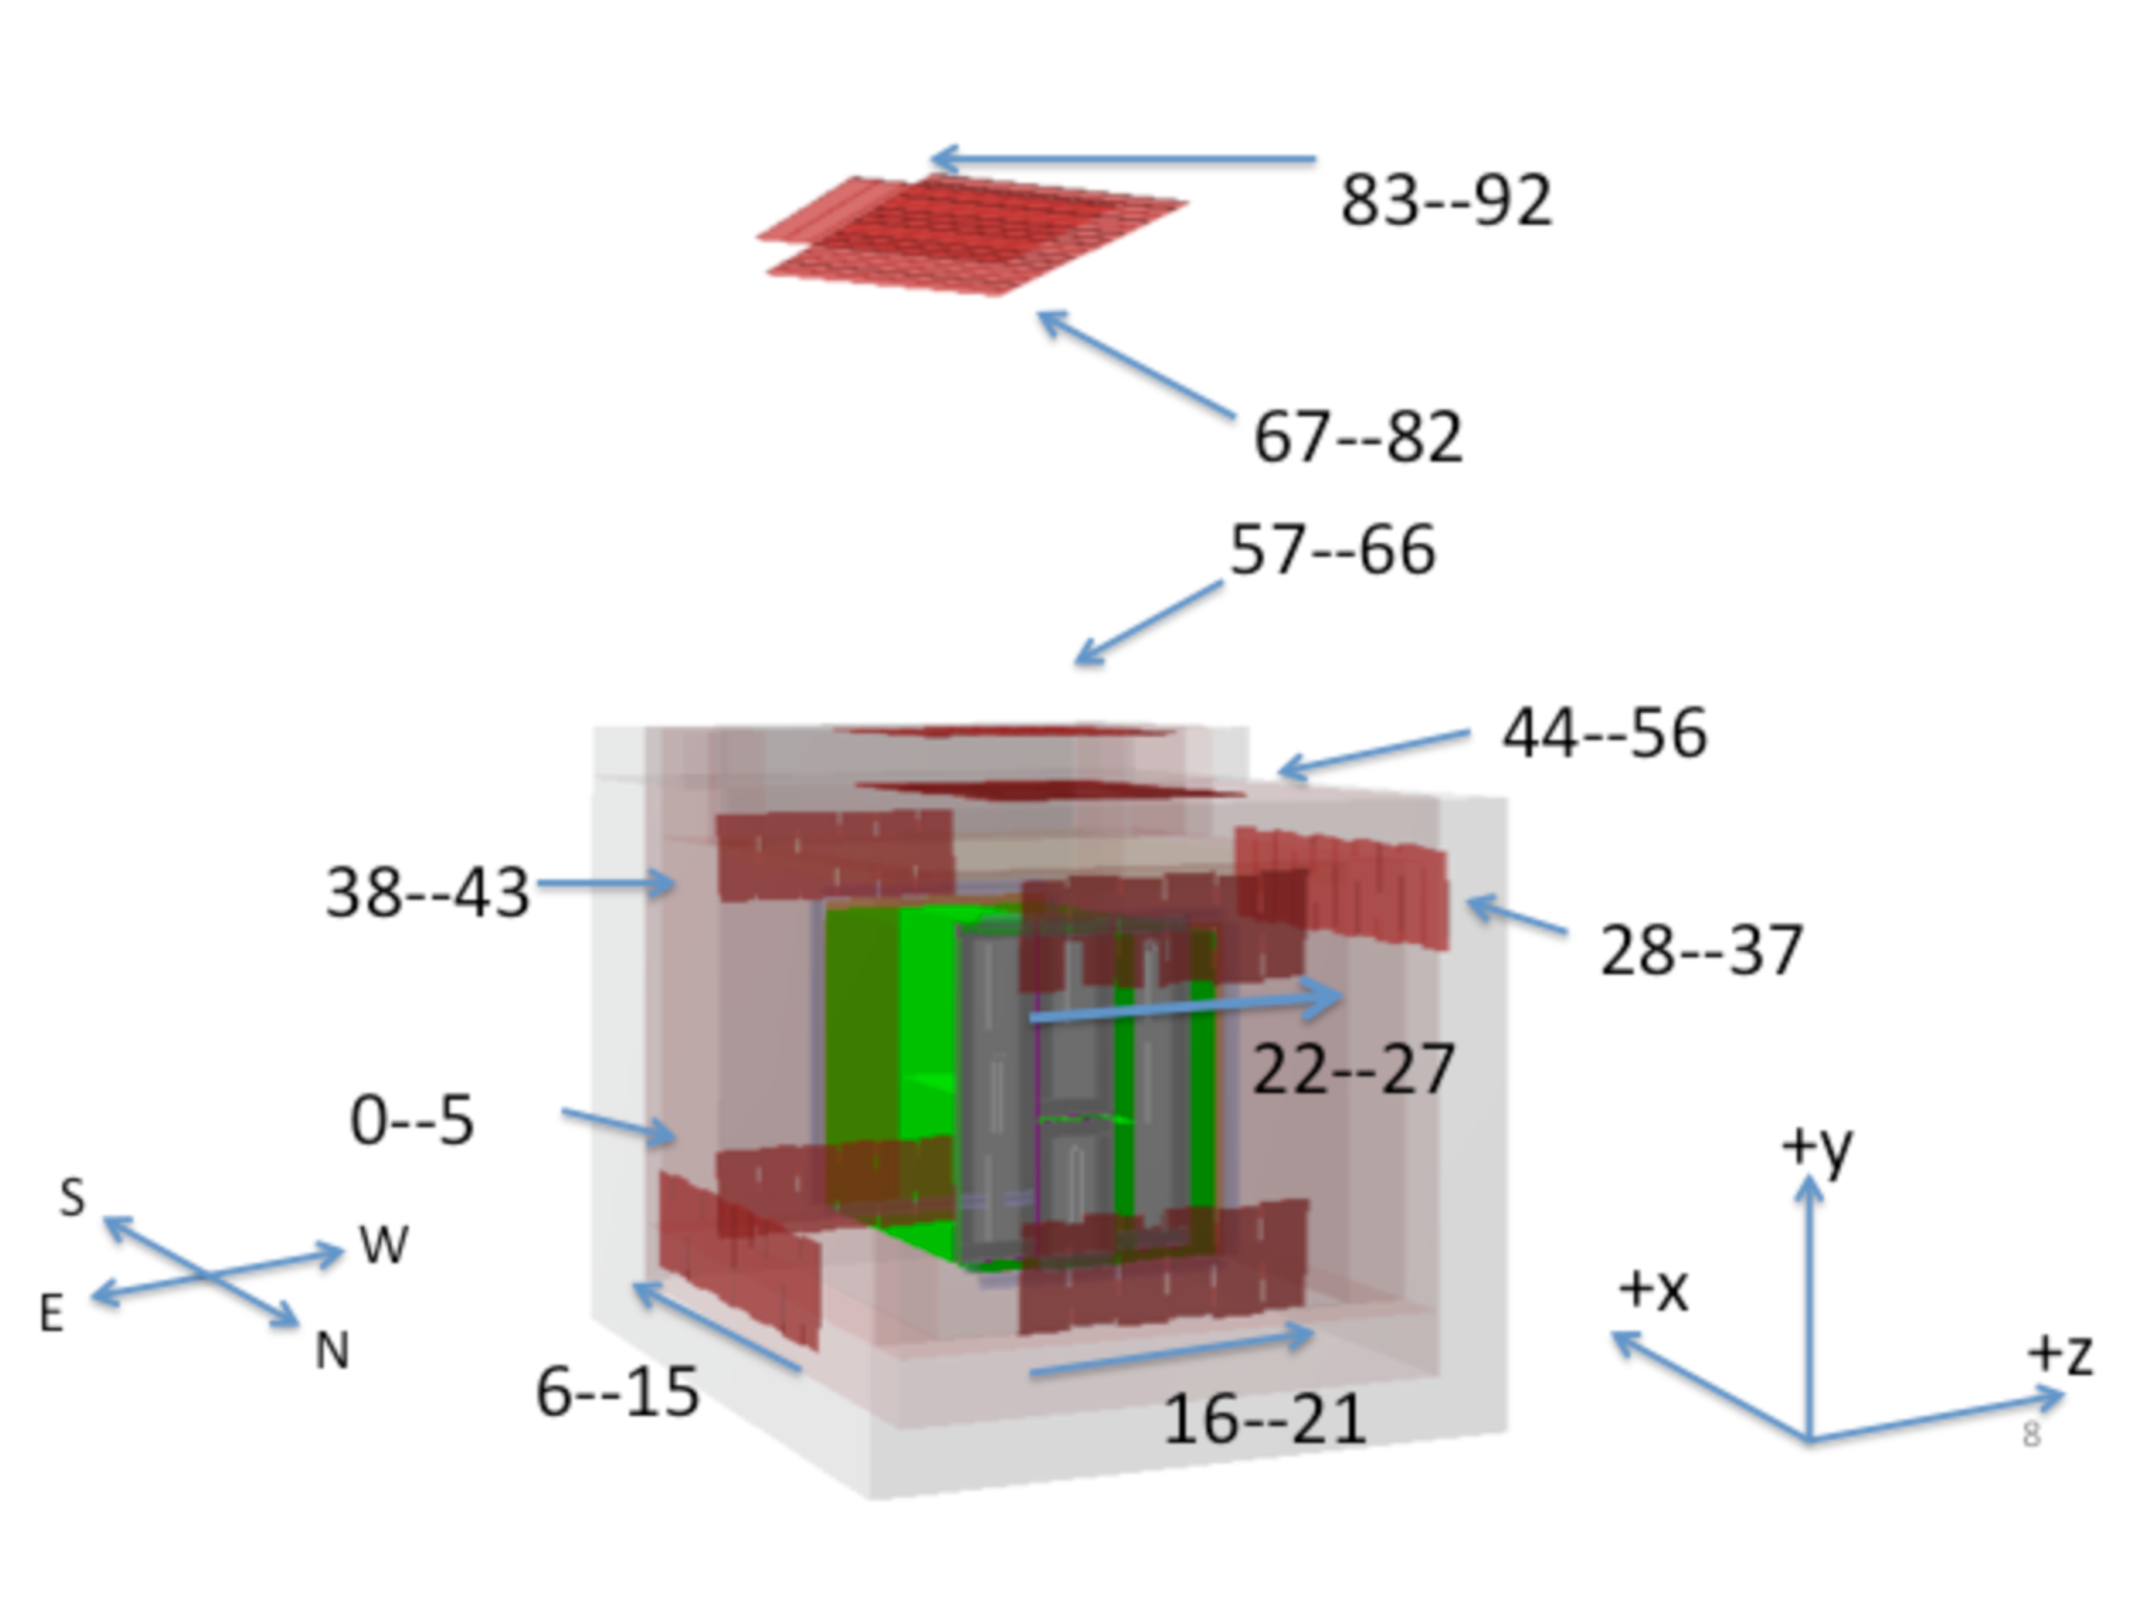
\includegraphics[width=0.85\textwidth]{35tonFullDetect}
  \caption[A representation of the counter locations in the 35 ton]
          {A representation of the counter locations in the 35 ton, with the magnetic, and LArSoft, co-ordinate systems shown. The other detector components can be seen inside the cryostat, such that the counters on the North wall are behind the short drift volume. The East - West counters are numbered 6-15 and 28-37 respectively. The North Lower - South Upper counters are numbered 16-21 and 38 - 43 respectively. The North Upper - South Lower counters are numbered 22-27 and 0-5 respectively. The ``telescope'' (vertically through-going) counters are numbered 44-92 and are split into four groups.}
  \label{fig:35tonCounterLoc}
\end{figure}

The Phase II run would build on the experience gained during the Phase I run, using the same process for the initial cooldown, and LAr recirculation. The run would also serve to show that the electron lifetime which could be achieved would not be limited by the presence of a detector. The operation of the installed TPC would also serve to test many of the novel features if the FD reference design. The results from the Phase II run are shown in Chapter~\ref{chap:35tonData}. \\

Following on from the 35 ton Phase II run is the single phase ProtoDUNE detector, which is due to take data in the second half of 2018. The ProtoDUNE detector is a scaled version of the full DUNE single phase reference design, as the APAs, and the drift length, are the same size as those in the reference design. The detector will be in a test beam, and so will be able to fully test the assumptions made in the DUNE CDRs about the detector performance characteristics. The detector will contain two sets of three APAs, 7.2 m apart, with one set of CPAs between them. This will give a total of 6 TPCs, each with a drift length of 3.6 m. \\

There is also a series of prototypes for the dual phase design. The WA105 project involves both a small scale demonstrator with an active mass of 1 $\times$ 3 $\times$ 3 m$^3$, which ran from late 2016 to early 2017, and a larger, scaled version of the dual phase design, the dual phase ProtoDUNE detector, measuring 6 $\times$ 6 $\times$ 6 m$^3$. As was the case with the single phase prototypes, the demonstrator is not in a beam and so has only taken cosmic data, whilst the larger detector is in a test beam, at the CERN neutrino platform. The larger detector will serve as a full scale demonstration of the dual phase detector design, though the drift distance is half of that in the final DUNE FD. Data-taking for this detector will be during the second half of 2018, at roughly the same time as the single phase ProtoDUNE detector. \\

%********************************** % Fifth Section  *************************************
\section{The DUNE software} \label{sec:LArSoft} %Section - X.5
The software package used by DUNE is called LArSoft~\citep{Church_LArSoft}~\citep{LArSoftOrg}. LArSoft is a simulation, reconstruction and analysis package for LArTPCs that is being used by many experiments in the US neutrino program. It has been developed to be detector agnostic, meaning that much of the code is shared between experiments. To this end, it is envisioned that it will be used as a platform for constant development in existing experiments, and those still in the planning phases, such as DUNE. LArSoft is built around the Fermilab-supported \emph{analysis reconstruction framework} (\emph{art}). External packages such as ROOT~\citep{ROOT} and GEANT4~\citep{GEANT4} are incorporated into LArSoft, meaning that the user does not have to coordinate specific versions of the packages. \\

There are numerous mechanisms by which particles can be generated within the software, as many external packages have been incorporated into the software. One such package is Generates Events for Neutrino Interaction Experiments (GENIE)~\citep{GENIE}, which is used to study neutrino interactions and nucleon decays. Another package, Nuance~\citep{Nuance}, is a neutrino interaction generator specifically for LAr. Finally, Cosmic-ray Shower Library (CRY)~\citep{CRY,CRY2}, and COsmic Ray SImulations for KAscade (CORSIKA)~\citep{CORSIKA}, are cosmic ray events generators, which are used to simulate the expected event rates for surface detector locations, in the absence of a neutrino beam. Recently the MUon Simulations UNderground (MUSUN)~\citep{MUSUN, MUSUN2} generator, which takes the output of MUon SImulation Code (MUSIC)~\citep{MUSUN, MUSIC, MUSIC2}, has also been incorporated, see Section~\ref{sec:FDIncorporation} for further details. It is also possible to use a single particle generator, where the particle type, initial momenta, initial positions, and initial directions, can all be set by the user. \\

The co-ordinates and angles in LArSoft are defined as follows;
\begin{itemize}
\item $x$ - The beam direction, with maximal $x$ being where the beam enters the detector.
  \begin{itemize}
  \item In the 35 ton prototype where there is no beam, positive $x$ is in the opposite direction to that which electrons drift in the large TPC, where $x$ = 0 is the position of the APA frames in the long drift volume.
  \item In the far detector geometry $x$ = 0 is defined as the midpoint between the two rows of CPAs 
  \end{itemize}
\item $y$ - The vertical direction, with maximal $y$ being the most highest point.
  \begin{itemize}
  \item In the 35 ton $y$ = 0 is halfway between the gap created by the two centre APAs, which are mounted one above the other.
  \item In the far detector $y$ = 0 is defined as the midpoint between the two vertical layers of TPCs.
  \end {itemize}
\item $z$ - Defined so as to have a right handed co-ordinate system.
  \begin{itemize}
  \item In both the 35 ton, and the far detector geometries, $z$ = 0 is at the edge of the leftmost (when looking down the long drift volume) APA frame.
  \end{itemize}
\item $\theta$ - The angle that a vector makes from the $x$ axis in the $xy$ plane.
\item $\phi$ - The angle between the $z$ axis and the vector.
\end{itemize}
Figure~\ref{fig:LArSoft_coords} shows a schematic representations of how the location of the origin appears in the 35 ton prototype.\\

\begin{figure}
  \centering
  \begin{subfigure}{0.48\textwidth}
    \centering
    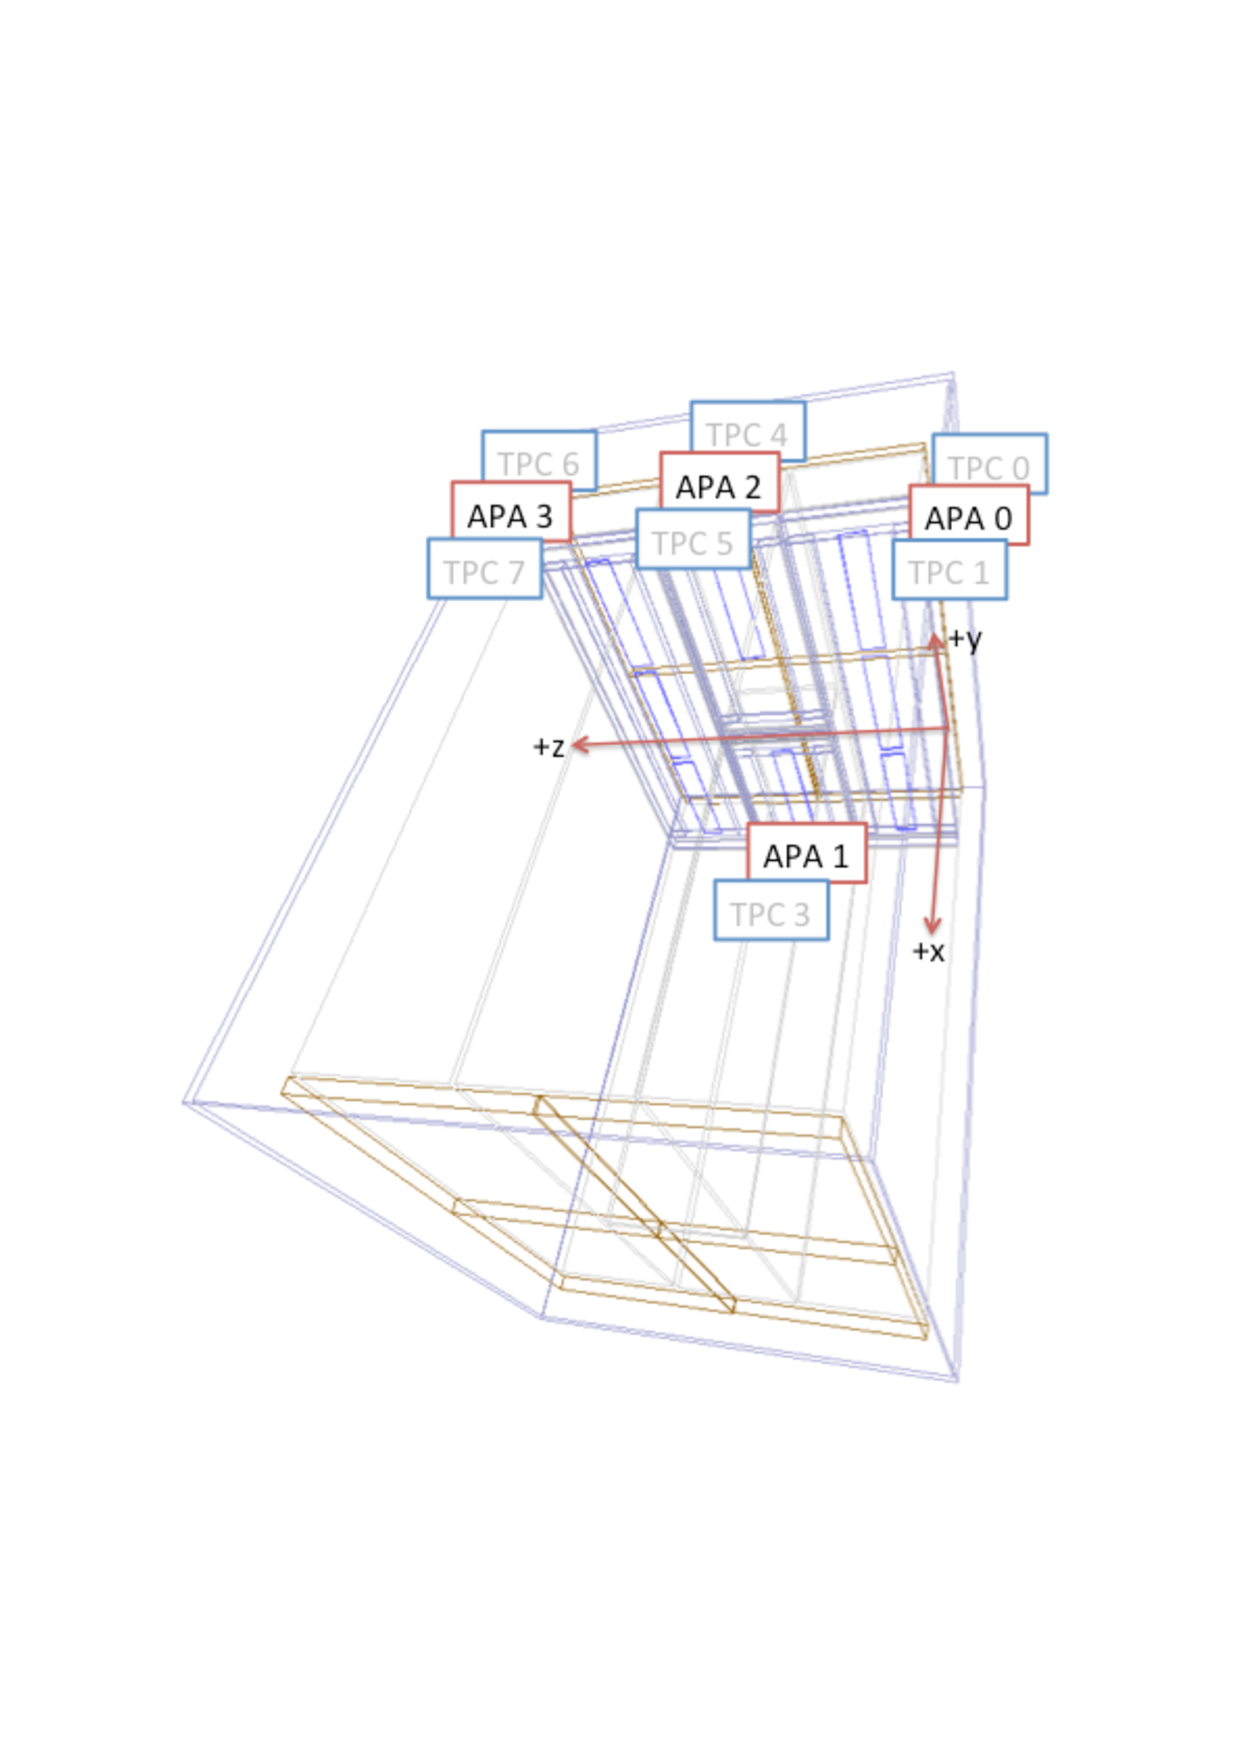
\includegraphics[width=\textwidth]{35ton_APASchem}
    \caption{The location of the origin of the 35 ton co-ordinate system in 3D.}
  \end{subfigure}%
  \begin{subfigure}{0.48\textwidth}
    \centering
    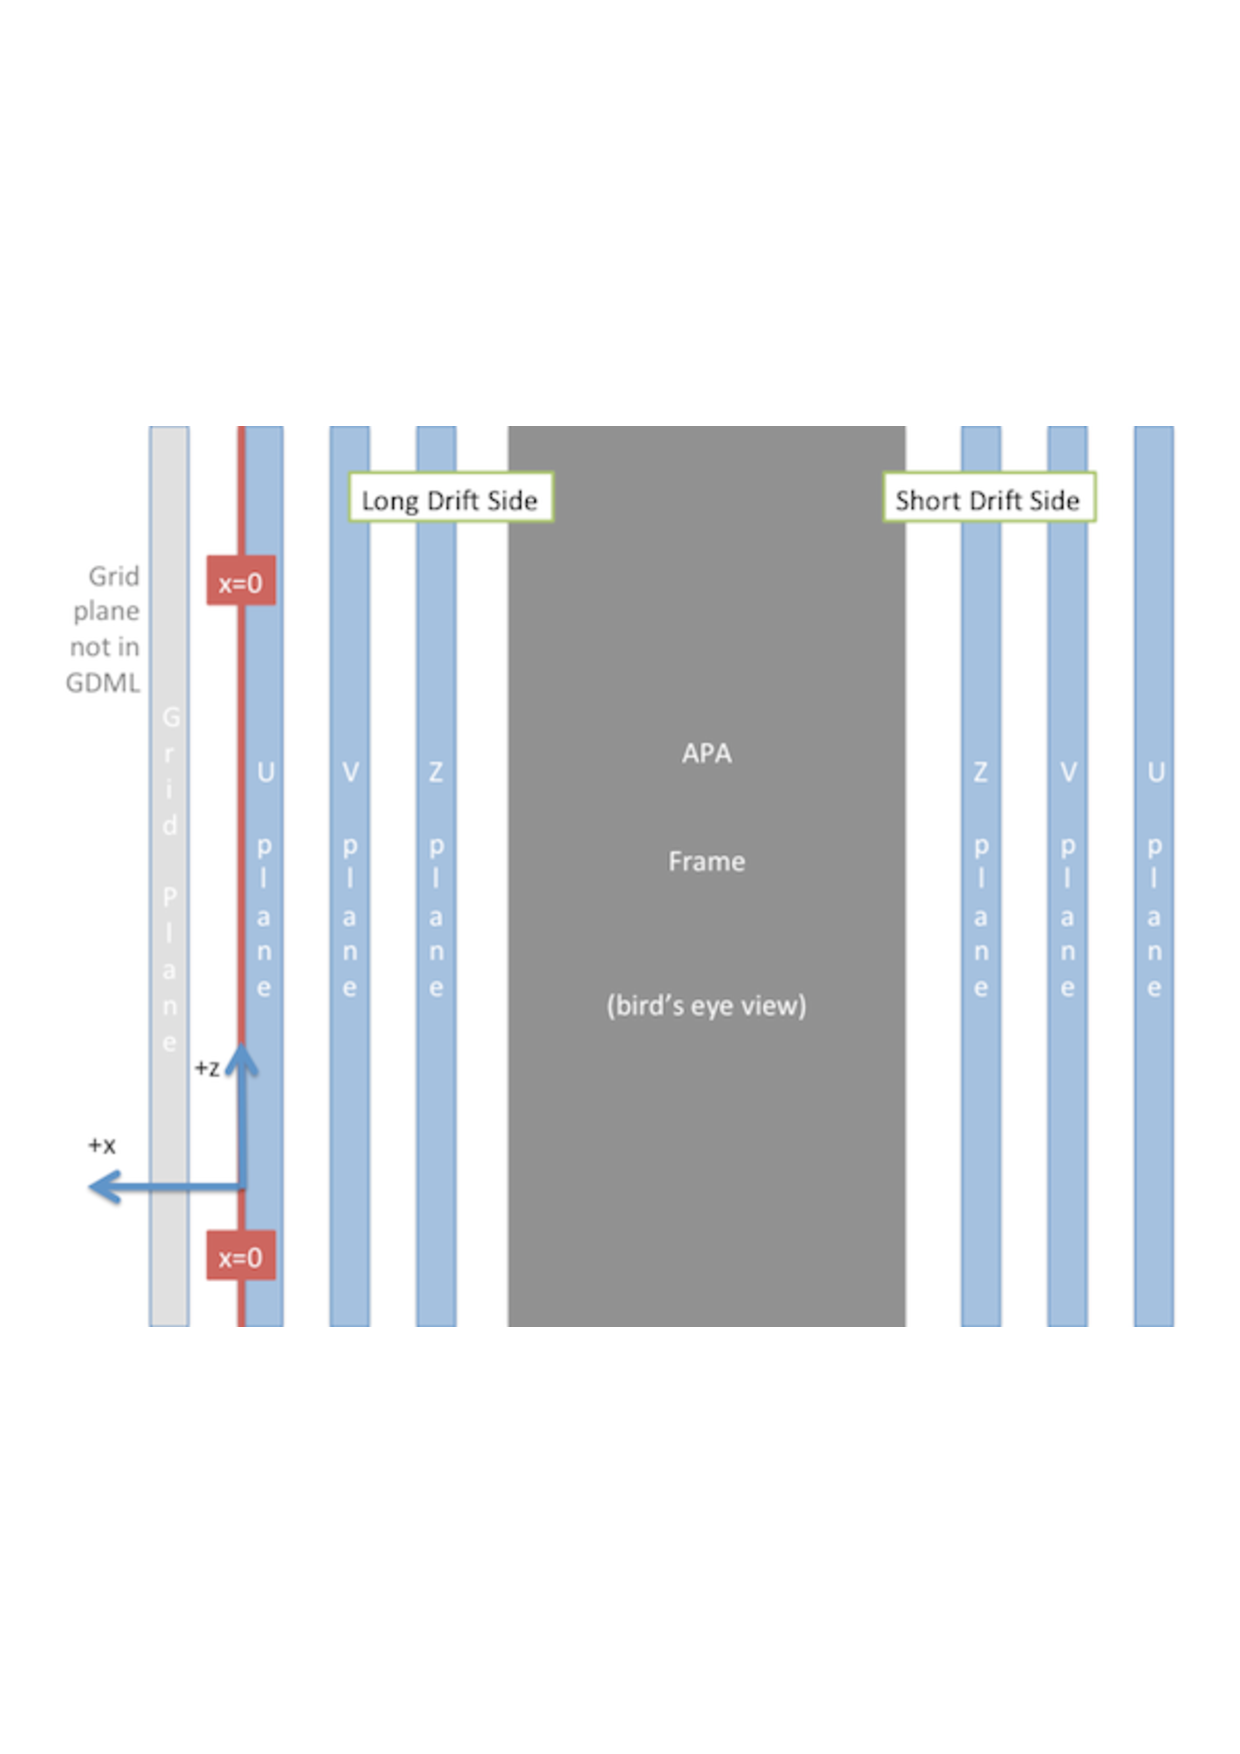
\includegraphics[width=\textwidth]{35ton_xCenter}
    \caption{The location of the origin of the 35 ton co-ordinate system in a 2D aerial view.}
  \end{subfigure}
  \caption[The LArSoft co-ordinate system as it is represented in the 35 ton.]
          {The LArSoft co-ordinate system as it is represented in the 35 ton. Left shows the location of the origin, relative to the TPC detector components. The four APAs, and eight TPCs are shown, where the even numbered TPCs are on the ``short'' drift side, 27 cm drift, and the odd numbered TPCs are on the ``long'' drift side, 223 cm drift. The CPAs (objects with a brown outline) are also shown. Right shows the location of the origin with respect to the APAs, and also shows the wire planes. It can be seen that $x$ = 0 is defined as the location of the U plane in the ``long'' drift volume. The figure is taken from~\citep{35tonGeomPage}.}
  \label{fig:LArSoft_coords}
\end{figure}

The simulation of particles is usually split into five processes, to reflect the different area in which development often progresses. These stages are as follows;
\begin{itemize}
\item Particle generator.
\item Particle transport using GEANT4.
\item Full detector simulation, including detector responses. 
\item Full event reconstruction.
\item Analysis.
\end{itemize}
The advantage of separating the computational processes in this way, is that improvements can be easily applied to a file without rerunning the entire simulation/reconstruction chain. This is especially important when large Monte Carlo, or data, samples are produced for general use within the collaboration, because it allows users to concentrate on improving a specific part of the computational process. When these all-purpose samples are produced a very general analysis is performed, which provides users with all of the Monte Carlo truth information, along with all of the reconstructed quantities. This general analysis produces a file which can be used outside of the LArSoft framework, so that users can perform analyses independently of LArSoft, should they wish to. \\

Later significant focus will be given to the reconstruction of TPC data, and so it is necessary to briefly illustrate the mechanisms by which TPC data is reconstructed in LArSoft. Much of the information presented below is summarised in~\citep{LArSoftOrg, LArSoftRecoNote}. The data collected by an experiment will have detector effects such as, an electronics response function, and a pedestal offset, present in the data. The full detector simulation also introduces these detector effects into simulated data, so that the reconstruction process does not treat simulated, and collected data, differently. The first step of the reconstruction algorithms is therefore, the removal of these detector effects. Once these effects are removed, the signal is estimated using the value of $signal/noise$ which would produce the measured signal. This process, called deconvolution, does not conserve pulse height, and is not guaranteed to preserve the normalisation. The deconvoluted signals are all unipolar distributions, which means that Gaussian distributions can be fitted to them, when trying to reconstruct hits. This is shown in Figure~\ref{fig:LotsOfHits}, and explained further below.\\

\begin{figure}
  \centering
  \begin{subfigure}{0.95\textwidth}
    \centering
    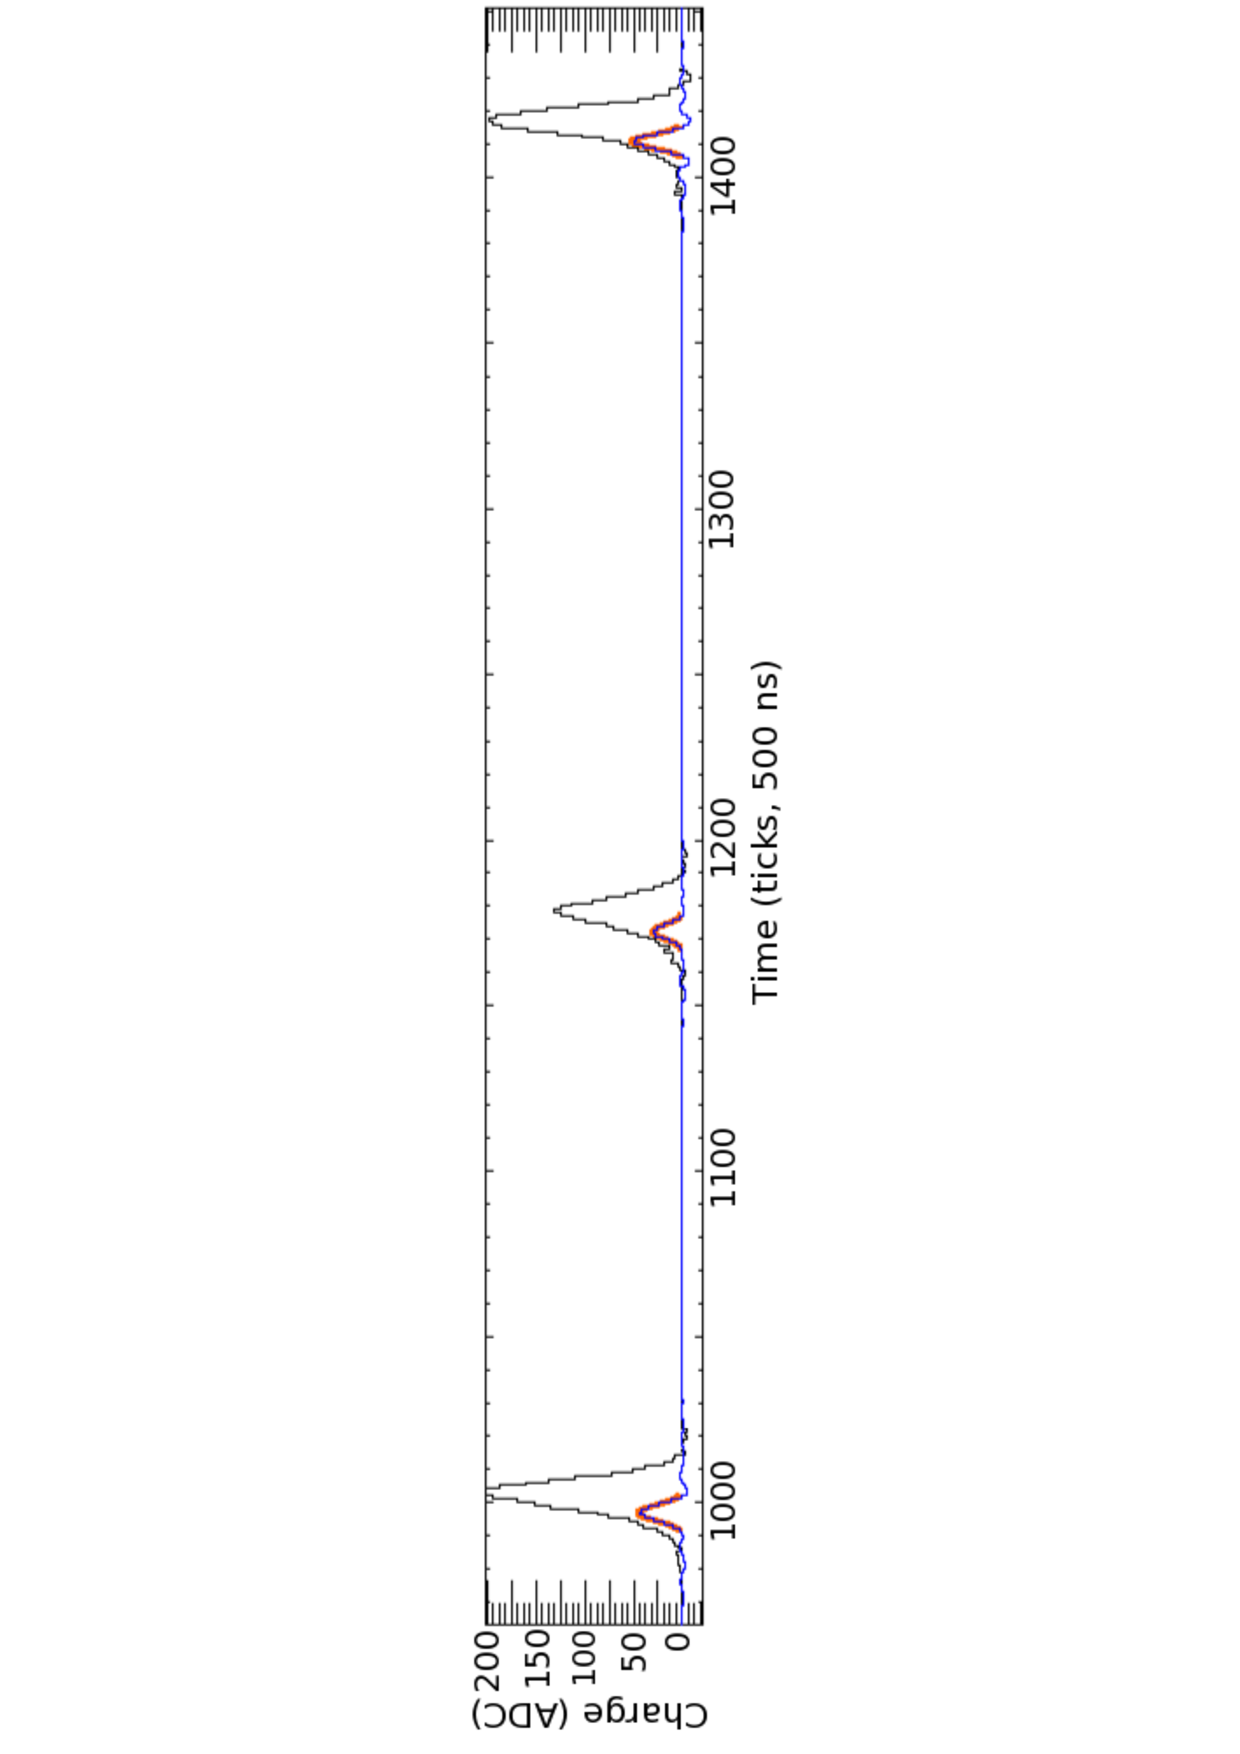
\includegraphics[width=\textwidth]{CollectionPlane}
    \caption{Collection plane depositions.}
    \label{fig:LotsOfHits_Col}
  \end{subfigure}
  \begin{subfigure}{0.95\textwidth}
    \centering
    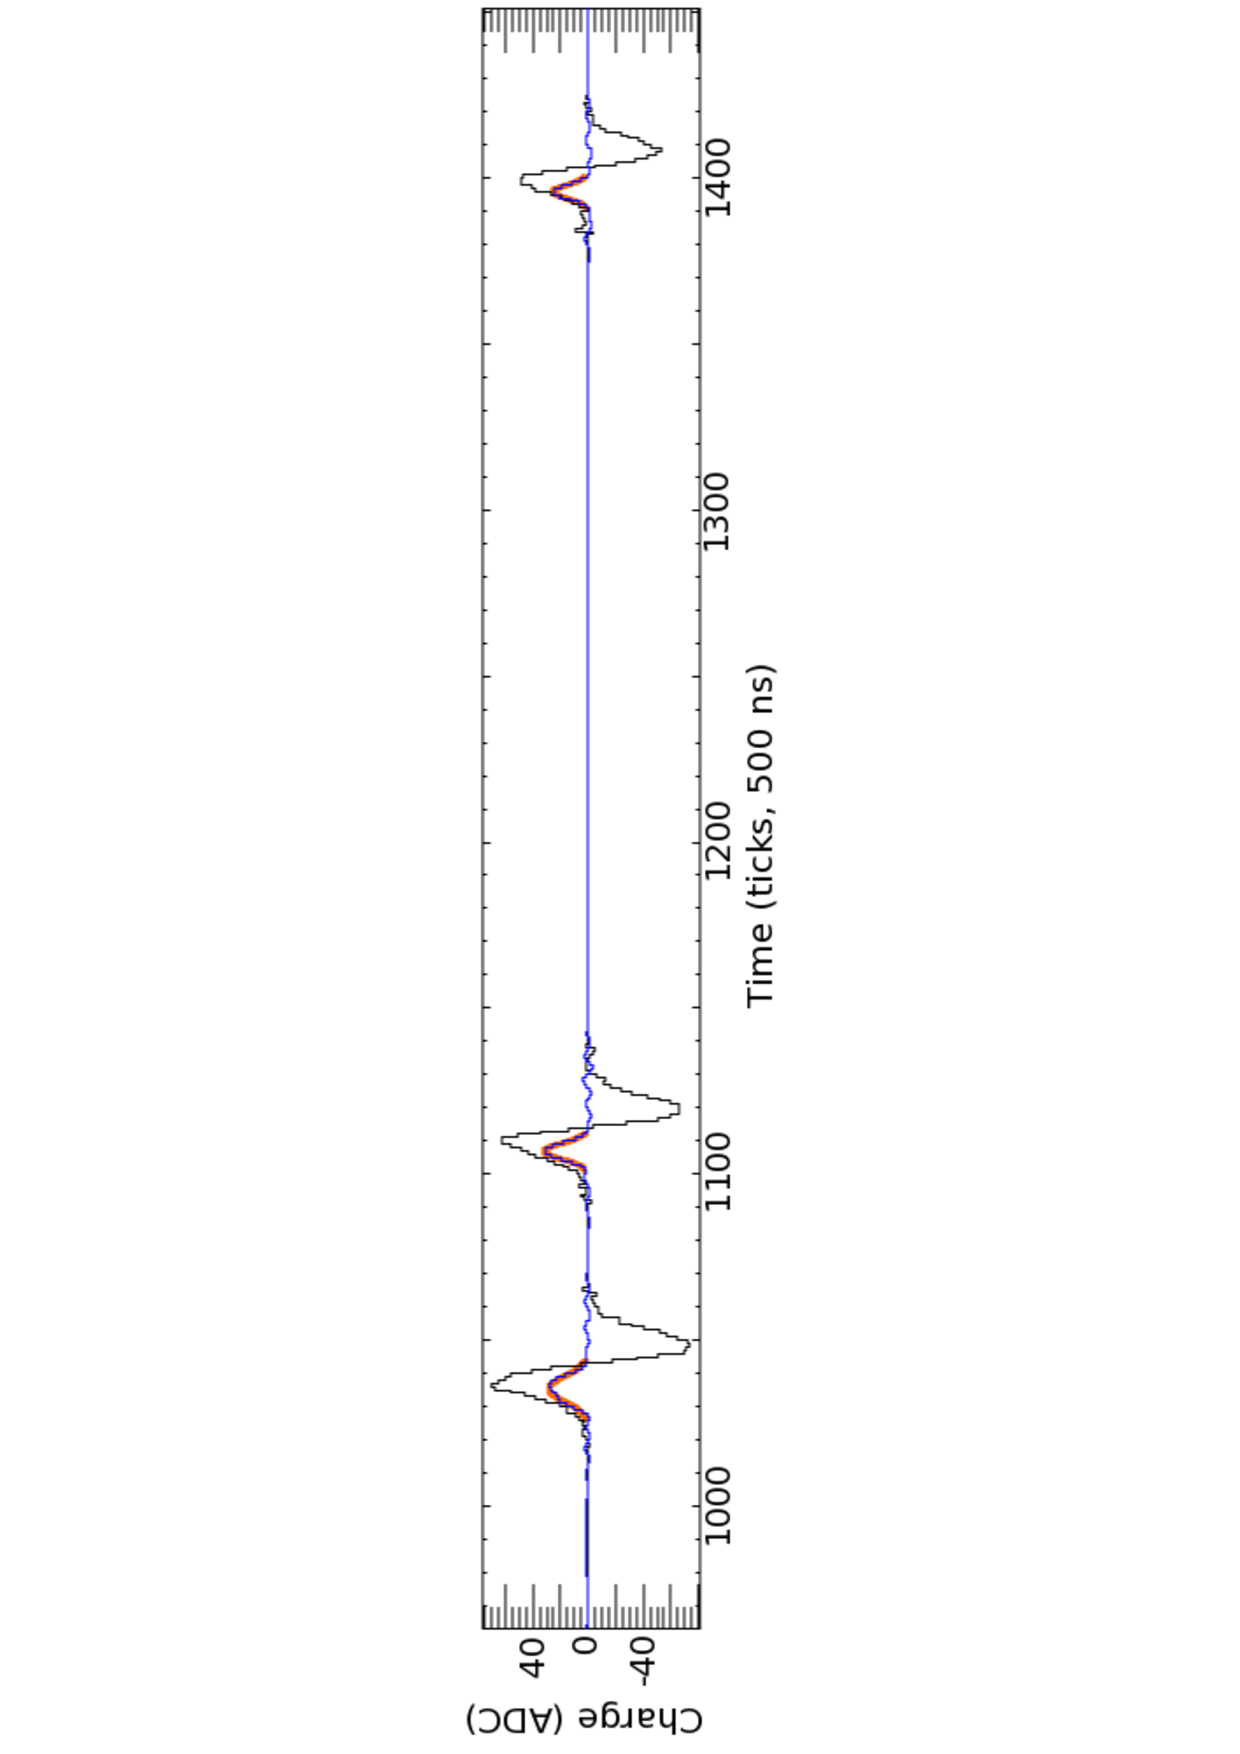
\includegraphics[width=\textwidth]{InductionPlane}
    \caption{Induction plane depositions.}
    \label{fig:LotsOfHits_Ind}
  \end{subfigure}
  \begin{subfigure}{0.95\textwidth}
    \centering
    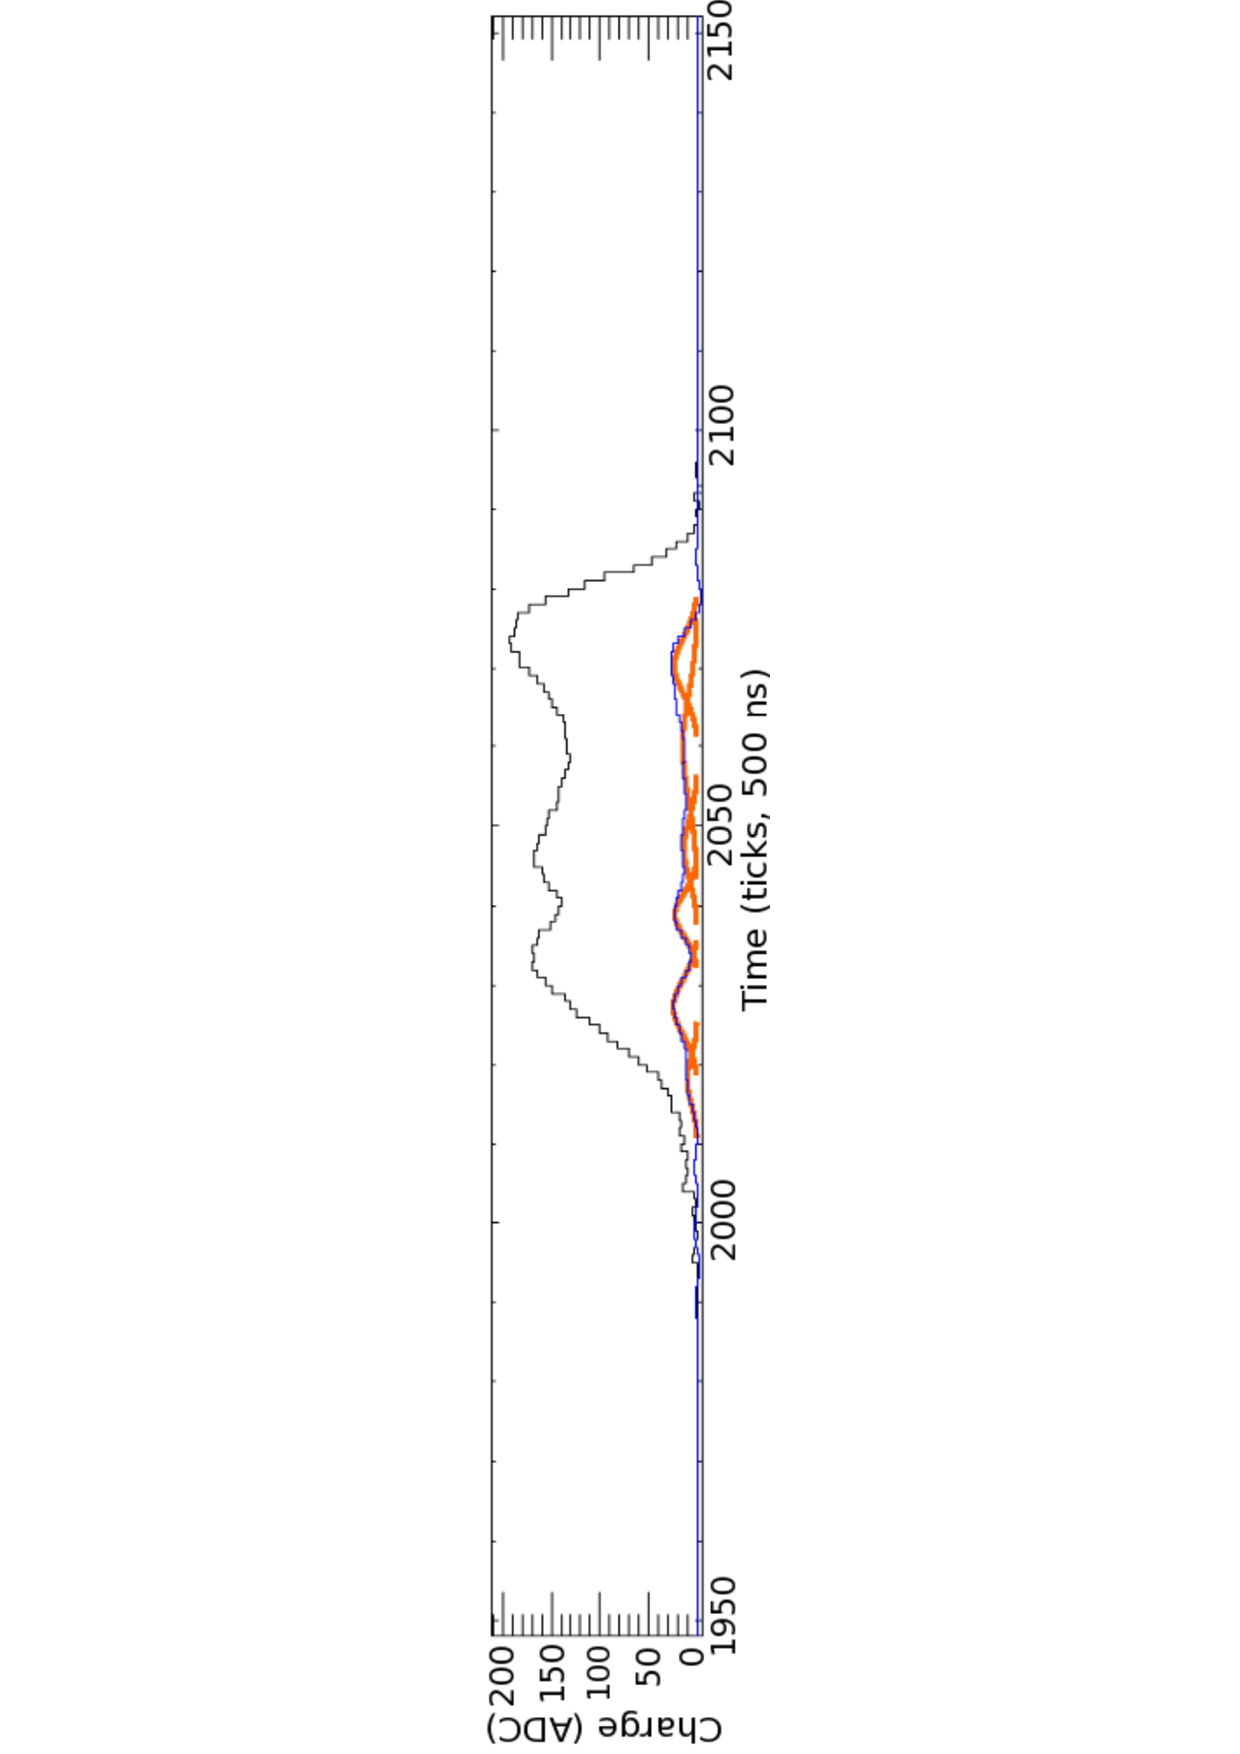
\includegraphics[width=\textwidth]{Complex}
    \caption{A large collection plane deposition over a large period of time.}
    \label{fig:LotsOfHits_Big}
  \end{subfigure}
  \caption[A selection of reconstructed hits, from simulated energy depositions]
          {The raw and deconvoluted signals, with reconstructed hits, for simulated energy depositions. The depositions, from particles generated by CRY, are not from a single event, and have been selected for demonstration purposes only. The plots are shown with increasing charge (ADC) on the $y$ axis, and increasing time (ticks, 500 ns) on the $x$ axis. The black lines represent the raw signals, the blue lines represent the deconvoluted signals, and the orange lines represent the reconstructed hits. Top shows depositions on a collection plane wire, it can be seen that the raw signal is unipolar. Middle shows depositions on an induction plane wire, it can be seen that the raw signal is bi-polar, whilst the deconvoluted signal, and reconstructed hits, are unipolar. Bottom shows a complex deposition on a collection plane wire, where multiple reconstructed hits are required to reproduce the deconvoluted signal.}
  \label{fig:LotsOfHits}
\end{figure}

The deconvoluted signals are reconstructed into hits by identifying regions that are above a threshold value, and then attempting to replicate the signal in these regions by introducing Gaussian distributions. For isolated hits, this is typically achieved using only one Gaussian distribution, however, for large energy depositions, over a large period time, where many particles are involved, multiple Gaussian distributions are often required. Large energy depositions are also possible when the direction of the particle aligns with the inclination of a wire plane, this means that all of the deposited energy may be deposited on a single wire. Examples of reconstructed hits are shown in Figure~\ref{fig:LotsOfHits}. These figures are taken from separate CRY simulated events, and so do not correspond to a continuous simulated event. They have been selected only as a demonstration of the process of hit reconstruction. Figures~\ref{fig:LotsOfHits_Col}, and~\ref{fig:LotsOfHits_Ind}, show multiple time-separated energy depositions on a collection plane wire, and an induction plane wire, respectively. A more complex energy deposition on a collection plane wire is shown in Figure~\ref{fig:LotsOfHits_Big}, where energy depositions from many particles, at similar times, have created a complicated energy deposition, which requires many reconstructed hits to explain. \\

As noted in Section~\ref{sec:DUNEDetector}, and Section~\ref{sec:The35tonDetector}, the DUNE FD, and the 35 ton, both have wrapped wires on the induction planes. A result of this, is that the location of the reconstructed hit on an induction wire is ambiguous, as a single wire has many wire segments, as shown in Figure~\ref{fig:35tonWireGeom}. An important feature of this ambiguity, is that the TPC in which the hit occurred cannot be identified, unless it is combined with another hit. These ambiguities do not extend to the collection plane wires, as they are not wrapped, and so consist of only a single wire segment, in a single TPC. Hits are combined across the three planes by identifying wire segments on each plane which intersect, and have hits at common times. In the traditional reconstruction process only hits that make these so-called 'triple points' are considered disambiguated, with other hits being identified as noise hits, causing them to be discarded. \\

The inclination of the wire planes has to be carefully chosen so as to minimise both the number of wires required, and the number of times that wire triplets intersect. This is shown in Figure~\ref{fig:WirePitches}, where the wire inclinations used in the 35 ton detector are compared to those in the DUNE FD reference design. The inclination of wires in the 35 ton was 45$^{\circ}$ $\pm$ 0.7$^{\circ}$, meaning that many wire triplets cross twice, and some wire pairs cross three times. When wire triplets cross multiple times, the triplet which has the smallest distance between the common intersection point, and the two-wire intersection points, is chosen as the location of the hit. This is shown as the 'Good intersection' on the right panel in Figure~\ref{fig:WirePitches}. The different wire pitches are necessary so that one of the triple points can be evaluated to be a better candidate for the hit location, as with a wire pitch of 45$^{\circ}$ it can be impossible to distinguish between different triple points. The inclination of wires in the FD was chosen to be 36$^{\circ}$ to remove the possibility of multiple intersection points, as given the geometry of the APAs, multiple intersection points are impossible, and so disambiguation is much simpler. The lower inclination results in more induction wires being required though, making it more expensive to instrument the detector. It is also important that all wires on a given APA are either read out at the top, or base, of the APA. This is because there must be minimal space between TPCs in the DUNE FD to reduce the internal dead space. As a result of this, APAs at the top of the cryostat are read out from the top of the APA, whilst APAs at the bottom of the cryostat are read out from the bottom of the APA. The APAs are never read out from the sides of the APAs, as the amount of cabling which would be required to do this, would cause a large amount of dead space between adjacent APAs. \\

\begin{figure}
  \centering
  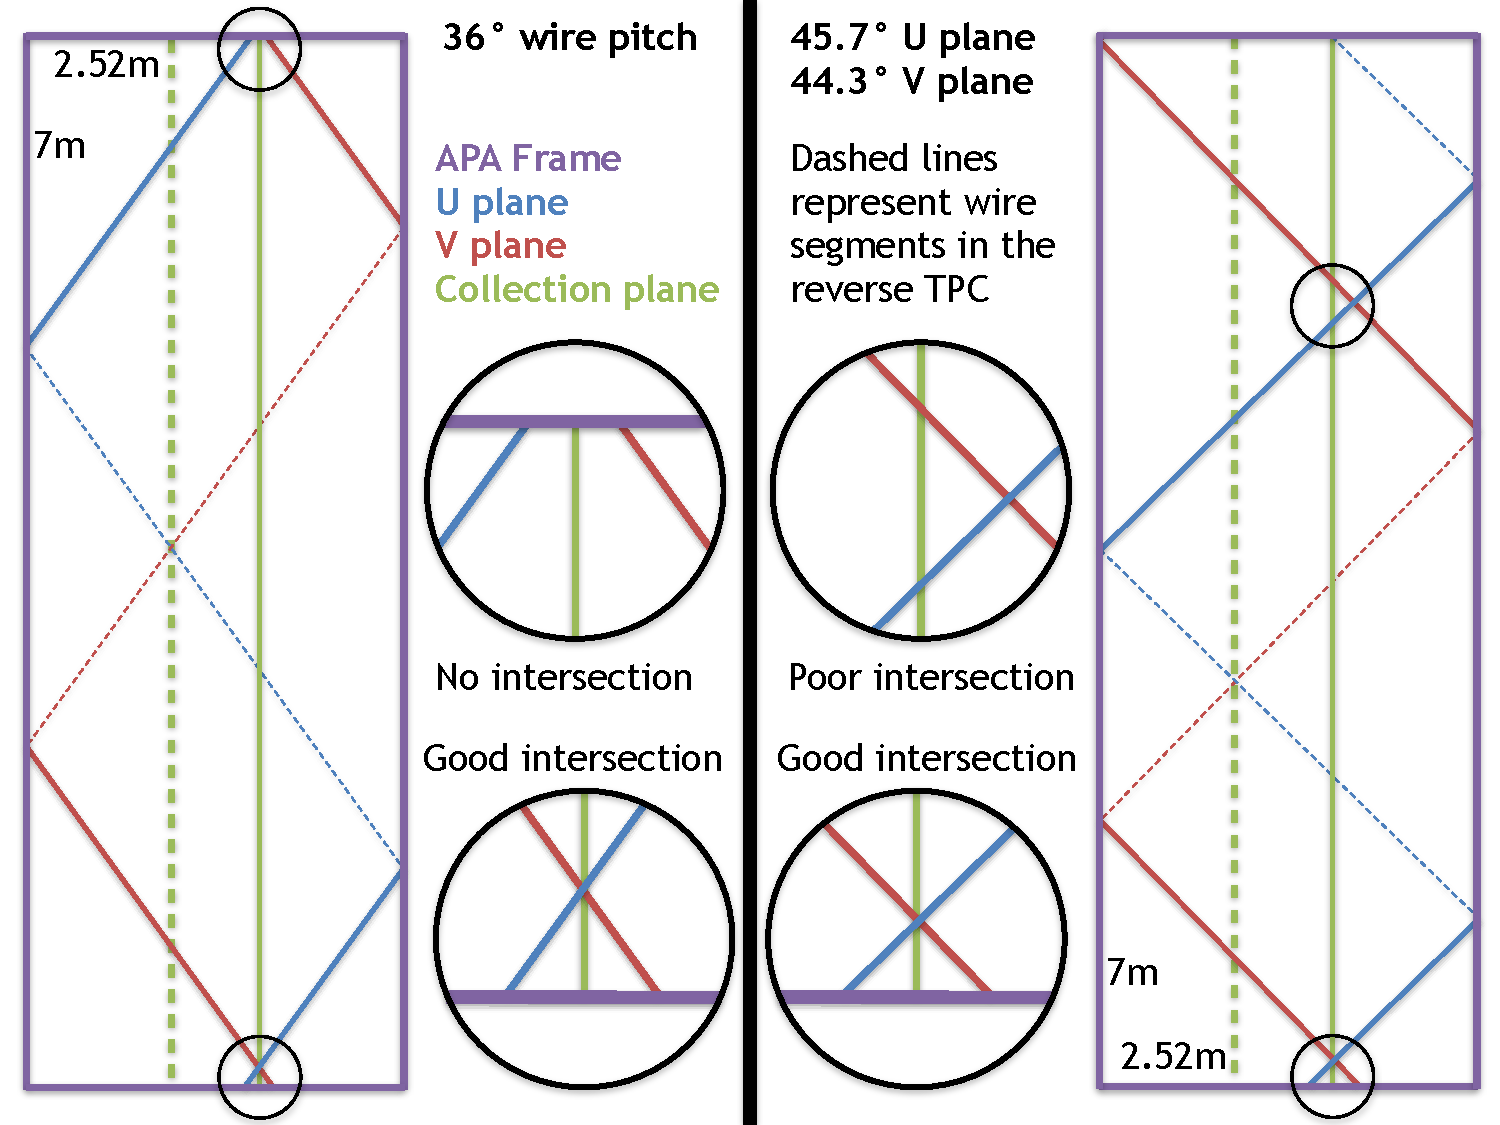
\includegraphics[width=0.85\textwidth]{WireAngleCondition}
  \caption[Performing disambiguation with different wire pitches.]
          {The effect that different wire pitches have on the ability to perform disambiguation in APAs with the far detector geometry. The left panel shows a wire pitch of 36$^{\circ}$, which is the reference design for the far detector, whilst the right panel shows wire pitches of 45$^{\circ}$ $\pm$ 0.7$^{\circ}$, as was used in the 35 ton. The left panel shows that only one 'triple point' can be made with the three wires shown, and so disambiguation is trivial. The right panel shows that two 'triple points' can be made with the three wires shown. The 'triple point' where the three wires have a common intersection point is labelled as a 'good intersection,' and it is this intersection point which would be chosen for the disambiguated hit.}
  \label{fig:WirePitches}
\end{figure}

Once the hits have been disambiguated they are combined to make clusters in each of the three planes. The clustering process is usually performed in wire-tick space on each plane separately, where all the hits from a single track or shower, should make a single cluster in each plane. It is possible to seed the start of clusters by using imaging techniques such as a Harris transform~\citep{HarrisTrans}, or to identify straight lines by using Hough transforms~\citep{HoughTrans}. As hits from a physical entity are unlikely to remain on a single channel, or all come at identical times, clusters are often spread out over many channels, for a range of times, especially when performing clustering for showers. \\

Once clusters have been identified in each plane, they can then be merged into 3-dimensional tracks and showers. The two most common tracking algorithms are PMTrack~\citep{PMTrack} and Pandora~\citep{Pandora}, and the most common showering algorithm is EMShower~\citep{EMShower}. Once 3D objects have been reconstructed, the calorimetric quantities need to be determined, this is often done separately for each plane. Two models exist for calculating $\frac{dE}{dx}$ in LArSoft, Birks model~\citep{BirksModel} and a modified Box model~\citep{PIDA_Paper}. The modified Box model uses a correction to the Box model~\citep{BoxModel} at low values of $\frac{dE}{dx}$. Normally the modified Box model is used, as it holds for both large and small ionisation's, whereas Birks model experiences difficulties at large ionisation's, and the traditional Box model struggles at low $\frac{dE}{dx}$. Both models incorporated in LArSoft calculate the $\frac{dE}{dx}$ of a hit using the deposited charge ($dQ$), and the track pitch ($dx$) of the hit, as well as the conversion of ADC value to number of electrons ($C_{GeV \rightarrow e^{-}}$), a correction due to electron lifetime ($C_{lifetime}$), the LAr density ($\rho$), the electric field ($E_{field}$), and the tuneable electron recombination factors ($Recomb_{X}$). The series of equations used in Birks model are shown in Equation~\ref{eq:Birks}, whilst those used in the modified Box model are shown in Equation~\ref{eq:ModBox}. \\

\begin{subequations}
  \label{eq:Birks}
  \begin{align}
    \frac{dE}{dx} &= \frac{ dQdx }{ \alpha - (\beta \times dQdx) } \label{eq:Birks_1} \\
    dQdx &= \frac{ dQ \times C_{lifetime} }{ dx \times C_{ADC \rightarrow e^{-}} } \label{eq:Birks_Correc} \\
    \alpha &= Recomb_{A} \times C_{GeV \rightarrow e^{-}} \times 10^{-3} \label{eq:Birks_A}\\
    \beta  &= \frac{ Recomb_{B} }{ \rho \times E_{field} } \label{eq:Birks_B}
  \end{align}
\end{subequations}

\begin{subequations}
  \label{eq:ModBox}
  \begin{align}
    \frac{dE}{dx} &= \frac{ e^{\alpha} - Recomb_{A} }{ \beta } \label{eq:ModBox_1} \\
    \alpha &= \frac{10^3 \times \beta }{ C_{GeV \rightarrow e^{-} } } \times \frac{dQ}{dx} \label{eq:ModBox_A}\\
    dQdx &= \frac{ dQ \times C_{lifetime} }{ dx \times C_{ADC \rightarrow e^{-}} } \label{eq:ModBox_Correc} \\
    \beta &= \frac{ Recomb_{B} }{ \rho \times E_{field} } \label{eq:ModBox_B}
  \end{align}
\end{subequations}

When performing calorimetry, it is also important that the interaction time is known, so that the $x$ positions of hits can be corrected, as they will be reconstructed assuming an interaction time of 0 s. This assumption is made, because when using beam events, the beam trigger is placed at a time of $T = 0$. An unknown interaction time causes the hit and track positions to be calculated incorrectly, and will also skew the calorimetric corrections, as recombination is a drift dependant effect.
